\documentclass{book}

\usepackage{tikz}
\usetikzlibrary{positioning, shapes, calc}
\usepackage{lipsum}
\usepackage{enumitem}

\usepackage{amsmath}
\usepackage{amssymb}
\usepackage{simpler-wick}
\usepackage{hyperref}
\usepackage{csquotes}
\usepackage{graphicx}
\usepackage{xcolor}
\usepackage{mathrsfs}

\title{Title}
\author{Author}
\date{\today}

\begin{document}
\maketitle

\tableofcontents

\chapter{lec01 202200204}

\emph{TODO before the lectures note, there are some content are from slides}

topics
\begin{enumerate}
    \item quantum harmonic oscillator
    \item creation and annihilation operators
    \item Fock space
    \item real space wave functions
    \item coherent state
    \item propagator
\end{enumerate}

goals
\begin{enumerate}
    \item QM warm-up
    \item do some Gaussian integrals
    \item change some basis
\end{enumerate}

As a warm-up, consider the QHO in one-dimension.
\begin{gather*}
    \hat{H}=\frac{\hat{p}^2}{2m}+\frac{1}{2}m\omega ^2\hat{x}^2 \\
    \left[ \hat{x},\hat{p} \right] =i\hbar \\
\end{gather*}
in position basis, $\hat{p}=-i\hbar \partial _x$. check
\begin{align*}
    \left[ \hat{x},\hat{p} \right] f\left( x \right) &=-i\hbar x\partial _xf+i\hbar \partial _x\left( xf \right) \\
    &=-i\hbar x\partial _xf+i\hbar f+i\hbar x\partial _xf\\
    &=i\hbar f
\end{align*}
In position basis, the eigenvalues satisfy
\[ -\frac{\hbar ^2}{2m}\partial _{x}^{2}\phi \left( x \right) +\frac{1}{2}m\omega ^2x^2\phi \left( x \right) =E\phi \left( x \right) \]
We can, however, solve it algebraically (without going to the position basis). First, let's adopt some dimensionless coordinates. We know $[\hat{H}]=[\hbar\omega]$; write
\[ \hat{H}=\frac{\hbar \omega}{2}\left( \frac{m\omega}{\hbar}\hat{x}^2+\frac{1}{m\hbar \omega}\hat{p}^2 \right) \]
Define
\[ \hat{X}=\sqrt{\frac{m\omega}{\hbar}}\hat{x},\quad \hat{P}=\frac{1}{\sqrt{m\hbar \omega}}\hat{p} \]
Then
\[ \left[ \hat{X},\hat{P} \right] =\sqrt{\frac{m\omega}{\hbar}}\frac{1}{\sqrt{m\hbar \omega}}\left[ \hat{x},\hat{p} \right] =i \]
Let's now define
\[ \hat{a}^{\dagger}=\frac{1}{\sqrt{2}}\left( \hat{X}-i\hat{P} \right) ,\quad \hat{a}=\frac{1}{\sqrt{2}}\left( \hat{X}+i\hat{P} \right) \]
which gives
\begin{gather*}
    \hat{a}^{\dagger}\hat{a}=\frac{1}{2}\left( \hat{X}-i\hat{P} \right) \left( \hat{X}+i\hat{P} \right) =\frac{1}{2}\left( \hat{X}^2+\hat{P}^2+i\left[ \hat{X},\hat{P} \right] \right) \\
    \hat{H}=\frac{\hbar \omega}{2}\left( \hat{X}^2+\hat{P}^2 \right) =\hbar \omega \left( \hat{a}^{\dagger}\hat{a}+\frac{1}{2} \right)
\end{gather*}
This gives a convenient way to construct the spectrum. First, check
\[ \left[ \hat{a},\hat{a}^{\dagger} \right] =\frac{1}{2}\left[ \hat{X}+i\hat{P},\hat{X}-i\hat{P} \right] =\frac{1}{2}i\left[ \hat{P},\hat{X} \right] -\frac{1}{2}i\left[ \hat{X},\hat{P} \right] =1 \]
So, if $\hat{H}|E\rangle =E|E\rangle$, we have
\begin{align*}
    \hat{H}\left( \hat{a}^{\dagger}|E\rangle \right) &=\hbar \omega \left( \hat{a}^{\dagger}\hat{a}+\frac{1}{2} \right) \hat{a}^{\dagger}|E\rangle \\
    &=\hbar \omega \left( \hat{a}^{\dagger}\hat{a}\hat{a}^{\dagger}+\frac{1}{2}\hat{a}^{\dagger} \right) |E\rangle \\
    &=\hbar \omega \left( \hat{a}^{\dagger 2}\hat{a}+\hat{a}^{\dagger}+\frac{1}{2}\hat{a}^{\dagger} \right) |E\rangle \\
    &=\hat{a}^{\dagger}\left( \hat{H}+\hbar \omega \right) |E\rangle \\
    &=\hat{a}^{\dagger}\left( E+\hbar \omega \right) |E\rangle \\
    &=\left( E+\hbar \omega \right) \left( \hat{a}^{\dagger}|E\rangle \right)
\end{align*}
which means $\hat{a}^{\dagger}|E\rangle$ is another eigenstate with energy $E+\hbar\omega$. This relates the different eigenstates. We just need to find the ground state. Since
\[ \langle \phi |\hat{a}^{\dagger}\hat{a}|\phi \rangle =\left\| \hat{a}|\phi \rangle \right\| ^2\ge 0,\quad \forall |\phi \rangle \]
If $\hat{a}$ has a null vector, then it will be the ground state. Let's just posit such a state exist, i.e.,
\[ \exists |0\rangle \quad \mathrm{s}.\mathrm{t}.\quad \hat{a}|0\rangle =0\]
Then the eigen spectrum is given by
\[ \left\{ |n\rangle ;E_n=\hbar \omega \left( n+\frac{1}{2} \right) \right\} \]
We can also find the matrix elements of $\hat{a},\hat{a}$ in this eigen basis. Recall
\[ |n+1\rangle =\mathcal{N} \hat{a}^{\dagger}|n\rangle \]
where $\mathcal{N}\in\mathbb{R}^+$ is the normalization factor. Also, from the preceding discussion we have
\[ \hat{a}^{\dagger}\hat{a}|n\rangle =n|n\rangle \]
The normalization is then
\begin{align*}
    1=\langle n+1|n+1\rangle &=\mathcal{N} ^2\langle n|\hat{a}\hat{a}^{\dagger}|n\rangle \\
    &=\mathcal{N} ^2\langle n|\left( \hat{a}^{\dagger}\hat{a}+1 \right) |n\rangle \\
    &=\left( n+1 \right) \mathcal{N} ^2
\end{align*}
\[ \hat{a}^{\dagger}|n\rangle =\sqrt{n+1}|n+1\rangle \]
similar argument gives $\hat{a}|n\rangle =\sqrt{n}|n-1\rangle$. In a matrix picture.
\[ \hat{a}^\dagger=\left[ \begin{matrix}{l}
	0&		&		&		&		\\
	1&		0&		&		&		\\
	&		\sqrt{2}&		0&		&		\\
	&		&		\sqrt{3}&		0&		\\
	&		&		&		\ddots&		\ddots\\
\end{matrix} \right] ,\quad \hat{a}=\left[ \begin{matrix}{l}
	0&		1&		&		&		\\
	&		0&		\sqrt{2}&		&		\\
	&		&		0&		\sqrt{3}&		\\
	&		&		&		0&		\ddots\\
	&		&		&		&		\ddots\\
\end{matrix} \right] \]
This is a ``number'' basis. We call it the Fock space. It's separable (but infinite dimensional). We are only left with showing $\hat{a}|0\rangle =0$ \emph{TODO-UNKNOWN-WORD} solution. To do so, let's go back to the position basis. Recall
\[ \hat{a}=\frac{1}{\sqrt{2}}\left( \hat{X}+i\hat{P} \right) =\frac{1}{\sqrt{2}}\left( X+i\left( -i\frac{\partial}{\partial X} \right) \right) =\frac{1}{\sqrt{2}}\left( X+\frac{\partial}{\partial X} \right) \]
\[ \hat{a}|\phi _0\rangle =0 \]
\[ \left( X+\frac{\partial}{\partial X} \right) \phi _0\left( X \right) =0 \]
\[ \int{\frac{d\phi _0\left( X \right)}{\phi _0\left( X \right)}}=-\int{XdX}\]
\[ \phi _0\left( X \right) =\mathcal{N} e^{-X^2/2}\]
Which is a Gaussian. Recall $X=\sqrt{\frac{m\omega}{\hbar}}x$,
\[ \phi _0\left( x \right) =\mathcal{N} e^{-m\omega x^2/\left( 2\hbar \right)} \]
To get the normalization,
\begin{align*}
    1&=\int_{-\infty}^{\infty}{\left| \phi _0\left( x \right) \right|}dx=\mathcal{N} ^2\int_{-\infty}^{\infty}{e^{-m\omega x^2/\hbar}dx}\\
    &=\mathcal{N} ^2\sqrt{\frac{\hbar}{2m\omega}}\int_{-\infty}^{\infty}{e^{-m\omega x^2/\hbar}\exp \left( -\left( \sqrt{\frac{\hbar}{2m\omega}}x \right) ^2/2 \right) d\left( \sqrt{\frac{\hbar}{2m\omega}}x \right)}\\
    &=\mathcal{N} ^2\sqrt{\frac{\hbar}{2m\omega}}\sqrt{2\pi}
\end{align*}
\[ \mathcal{N} =\left( \frac{m\omega}{\pi \hbar} \right) ^{1/4} \]
\[ \phi _0\left( x \right) =\left( \frac{m\omega}{\pi \hbar} \right) ^{1/4}e^{-m\omega x^2/\left( 2\hbar \right)} \]
Side note: Gaussian integration
\[ \int_{-\infty}^{\infty}{e^{-ax^2/2}dx}=\sqrt{\frac{2\pi}{a}},\quad a>0 \]
A standard discussion will next introduce the real-space wave function of the excited states through the Hermite polynomial. Let's try to avoid that!

\section{coherent state}

We have seen that the creation and annihilation operatos provides a simple way to analyze the QHO. Let's now take these as the ``coordinates'' for our problem. Recall position basis $\hat{x}|x\rangle =x|x\rangle$. Similarly, we consider the eigenstates of the form
\[ \hat{a}|\alpha \rangle =\alpha |\alpha \rangle ;\quad \alpha \in \mathbb{C} \]
E.g., The ground state $\hat{a}|0\rangle =0|0\rangle =0$. To solve for the eigenstate, write
\[ |\alpha \rangle =\sum_{n=0}{C_n\left( \alpha \right) |n\rangle}\]
Then,
\begin{align*}
    \hat{a}|\alpha \rangle &=\sum_{n=0}{C_n\left( \alpha \right) \hat{a}|n\rangle}\\
    &=\sum_{n=0}{C_n\left( \alpha \right) \sqrt{n}|n-1\rangle}\\
    &=\sum_{n=0}{C_{n+1}\left( \alpha \right) \sqrt{n+1}|n\rangle}\\
\end{align*}
versus
\[ \alpha |\alpha \rangle =\sum_{n=0}{C_n\left( \alpha \right) \alpha |n\rangle}\]
we conclude
\[ C_{n+1}\left( \alpha \right) =\frac{\alpha C_n\left( \alpha \right)}{\sqrt{n+1}}=\frac{\alpha ^2C_{n-1}\left( \alpha \right)}{\sqrt{\left( n+1 \right) n}}=\cdots =\frac{\alpha ^{n+1}C_0\left( \alpha \right)}{\sqrt{\left( n+1 \right) !}} \]

Note: $|\alpha\rangle$ is a superposition of $\{|n\rangle\}$. It's not an energy eigenstate (unless $\alpha=0$).

We have
\[ |\alpha \rangle =C_0\left( \alpha \right) \sum_{n=0}{\frac{\alpha ^n}{\sqrt{n!}}|n\rangle}\]
Normalization:
\begin{align*}
    1&=\langle \alpha |\alpha \rangle =\left| C_0\left( \alpha \right) \right|^2\sum_{m,n=0}{\frac{\left( \alpha ^* \right) ^m\alpha ^n}{\sqrt{m!}\sqrt{n!}}\langle m|n\rangle}\\
    &=\left| C_0\left( \alpha \right) \right|^2\sum_{m=0}{\frac{\left| \alpha \right|^{2m}}{m!}}\\
    &=\left| C_0\left( \alpha \right) \right|^2e^{\left| \alpha \right|^2}
\end{align*}
\[ C_0\left( \alpha \right) =e^{-\left| \alpha \right|^2/2}\]
\[ |\alpha \rangle =e^{-\left| \alpha \right|^2/2}\sum_{n=0}{\frac{\alpha ^n}{\sqrt{n!}}|n\rangle}\]
This looks almost like the exponential! Recall
\[ |n\rangle =\frac{\hat{a}^{\dagger}}{\sqrt{n}}|n-1\rangle =\frac{\hat{a}^{\dagger 2}}{\sqrt{n\left( n-1 \right)}}|n-2\rangle =\cdots =\frac{\hat{a}^{\dagger n}}{\sqrt{n!}}|0\rangle \]
So,
\begin{align*}
    |\alpha \rangle &=e^{-\left| \alpha \right|^2/2}\sum_{n=0}{\frac{\alpha ^n\hat{a}^{\dagger n}}{\sqrt{n!}\sqrt{n!}}|0\rangle}\\
    &=e^{-\left| \alpha \right|^2/2}e^{\alpha \hat{a}^{\dagger}}|0\rangle
\end{align*}


\chapter{lec02 202200209}

topics:

\begin{enumerate}
    \item QHO: displacement operator and propagator
    \item Phonons: from QHO to second quantization
\end{enumerate}

goals

\begin{enumerate}
    \item continue with our QM warm-up
    \item introduce the propagator, Green function
    \item free phonons as our first ``many-body'' bosonic problem
\end{enumerate}

\section{QHO}

Recall the QHO Hamiltonian

\begin{gather*}
    \hat{H}=\frac{\hat{p}^2}{2m}+\frac{1}{2}m\omega ^2\hat{x}^2=\hbar \omega \left( \hat{a}^{\dagger}\hat{a}+\frac{1}{2} \right) \\
    \hat{a}=\frac{1}{\sqrt{2}}\left( \hat{X}+i\hat{P} \right) \\
    \hat{X}=\sqrt{\frac{m\omega}{\hbar}}\hat{x}\\
    \hat{P}=\frac{1}{\sqrt{m\hbar \omega}}\hat{p}
\end{gather*}
Coherent states are labeled by $\alpha\in\mathcal{C}$
\[ \hat{a}|\alpha \rangle =\alpha |\alpha \rangle \]

Displacement operator: unitary to rotate between coherent states, let
\[ \hat{D}\left( \alpha \right) =e^{ \alpha \hat{a}^{\dagger}-\alpha ^*\hat{a} } \]
where $\alpha \hat{a}^{\dagger}-\alpha ^*\hat{a}$ is anti-Hermitian.

Baker-Campbell-Hausdorff formula: for $[\hat{A},\hat{B}]$ central ($[\hat{A},\hat{B}]$ commutes with both $\hat{A}\&\hat{B}$)
\[ e^{\hat{A}}e^{\hat{B}}=e^{\hat{A}+\hat{B}+\frac{1}{2}\left[ \hat{A},\hat{B} \right]}\]
By BCH, and noting $\left[ \alpha \hat{a}^{\dagger},-\alpha ^*\hat{a} \right] =\left| \alpha \right|^2$ is central,
\begin{gather*}
    e^{\alpha \hat{a}^{\dagger}}e^{-\alpha ^*\hat{a}}=e^{\alpha \hat{a}^{\dagger}-\alpha ^*\hat{a}}e^{\left[ \alpha \hat{a}^{\dagger},-\alpha ^*\hat{a} \right] /2}\\
    \hat{D}\left( \alpha \right) =e^{\alpha \hat{a}^{\dagger}-\alpha ^*\hat{a}}=e^{-\left| \alpha \right|^2/2}e^{\alpha \hat{a}^{\dagger}}e^{-\alpha ^*\hat{a}}
\end{gather*}
Check
\[ \hat{D}\left( \alpha \right) |0\rangle =e^{-\left| \alpha \right|^2/2}e^{\alpha \hat{a}^{\dagger}}e^{-\alpha ^*\hat{a}}|0\rangle =e^{-\left| \alpha \right|^2/2}e^{\alpha \hat{a}^{\dagger}}|0\rangle =|\alpha \rangle \]
``Displacement''? compute (also using BCH formula)
\begin{align*}
    \hat{D}^{\dagger}\left( \alpha \right) \hat{a}\hat{D}\left( \alpha \right) &=e^{-\alpha \hat{a}^{\dagger}+\alpha ^*\hat{a}}\hat{a}e^{\alpha \hat{a}^{\dagger}-\alpha ^*\hat{a}}\\
    &=\hat{a}+\left[ -\alpha \hat{a}^{\dagger}+\alpha ^*\hat{a},\hat{a} \right] \\
    &=\hat{a}+\alpha
\end{align*}
\[ \hat{D}^{\dagger}\left( \alpha \right) \hat{a}^{\dagger}\hat{D}\left( \alpha \right) =\hat{a}^{\dagger}+\alpha ^*\]

E.g., 1. Average energy
\begin{align*}
    \langle \alpha |\hat{H}|\alpha \rangle &=\langle 0|\hat{D}^{\dagger}\left( \alpha \right) \hbar \omega \left( \hat{a}^{\dagger}\hat{a}+\frac{1}{2} \right) \hat{D}\left( \alpha \right) |0\rangle \\
    &=\langle 0|\hbar \omega \left( \left( \hat{a}^{\dagger}+\alpha ^* \right) \left( \hat{a}+\alpha \right) +\frac{1}{2} \right) |0\rangle \\
    &=\frac{\hbar \omega}{2}+\hbar \omega \langle 0|\left( \hat{a}^{\dagger}\hat{a}+\hat{a}^{\dagger}\alpha +\alpha ^*\hat{a}+\left| \alpha \right|^2 \right) |0\rangle \\
    &=\hbar \omega \left( \left| \alpha \right|^2+\frac{1}{2} \right)
\end{align*}
Not an eigenstate, and has a continuously adjustable average energy.

E.g., 2. Expectation values for $\langle \hat{x}\rangle$ and $\langle \hat{p}\rangle$
\[ \alpha =\langle \alpha |\left( \hat{X}+i\hat{P} \right) |\alpha \rangle =\frac{1}{\sqrt{2}}\langle \alpha |\hat{X}|\alpha \rangle +\frac{i}{\sqrt{2}}\langle \alpha |\hat{P}|\alpha \rangle \]
It's natural for us to parametrize the complex variable
\[ \alpha =\frac{1}{\sqrt{2}}\left( X_{\alpha}+iP_{\alpha} \right) ,X_{\alpha},P_{\alpha}\in \mathbb{R} \]
and simply the expectation values
\begin{gather*}
    X_{\alpha}=\langle \alpha |\hat{X}|\alpha \rangle =\sqrt{\frac{m\omega}{\hbar}}\langle \alpha |\hat{x}|\alpha \rangle \\
    P_{\alpha}=\langle \alpha |\hat{P}|\alpha \rangle =\frac{1}{\sqrt{m\hbar \omega}}\langle \alpha |\hat{P}|\alpha \rangle
\end{gather*}
In particular, the ground state for the shifted Hamiltonian
\[ \hat{H}'=\frac{\hat{p}^2}{2m}+\frac{1}{2}m\omega ^2\left( \hat{x}-x_0 \right) ^2\]
will be the coherent state $\hat{D}(\sqrt{\frac{m\omega}{\hbar}}x_0)|0\rangle$.

E.g., 3. Composition of displacement operator

We can think of $\hat{D}(\alpha)$ as a ``displacement'' in the phase space. It is natural to look how such transformation compose.
\begin{align*}
    \hat{D}\left( \alpha \right) \hat{D}\left( \beta \right) &=e^{\alpha \hat{a}^{\dagger}-\alpha ^*\hat{a}}e^{\beta \hat{a}^{\dagger}-\beta ^*\hat{a}}\\
    &=e^{\left( \alpha +\beta \right) \hat{a}^{\dagger}-\left( \alpha ^*+\beta ^* \right) \hat{a}}e^{\left[ \alpha \hat{a}^{\dagger}-\alpha ^*\hat{a},\beta \hat{a}^{\dagger}-\beta ^*\hat{a} \right] /2}\\
    &=\hat{D}\left( \alpha +\beta \right) e^{\frac{1}{2}\left( -\alpha ^*\beta \left[ \hat{a},\hat{a}^{\dagger} \right] -\alpha \beta ^*\left[ \hat{a}^{\dagger},\hat{a} \right] \right)}\\
    &=\hat{D}\left( \alpha +\beta \right) e^{\left( \alpha \beta ^*-\alpha ^*\beta \right) /2}\\
    &=\hat{D}\left( \alpha +\beta \right) e^{i\mathrm{Im}\left( \alpha \beta ^* \right)}
\end{align*}
Note:
\[ \hat{D}\left( \alpha \right) \hat{D}\left( -\alpha \right) =\hat{D}\left( 0 \right) =I\quad \Rightarrow \quad \hat{D}^{\dagger}\left( \alpha \right) =\hat{D}\left( -\alpha \right) \]

Overlap between coherent states: we now see that coherent states are \emph{not} orthogonal:
\begin{align*}
    \langle \alpha |\beta \rangle &=\langle 0|\hat{D}^{\dagger}\left( \alpha \right) \hat{D}\left( \beta \right) |0\rangle \\
    &=\langle 0|\hat{D}\left( -\alpha +\beta \right) |0\rangle e^{-i\mathrm{Im}\left( \alpha \beta ^* \right)}\\
    &=e^{-\left| \alpha -\beta \right|^2/2}e^{-i\mathrm{Im}\left( \alpha \beta ^* \right)}\\
    &=e^{-\left( \left| \alpha \right|^2+\left| \beta \right|^2 \right) /2}e^{\alpha ^*\beta}
\end{align*}
we usually say they form an over-complete basis.

Resolution of identity
\begin{align*}
    \int{d^2\alpha \langle n|\alpha \rangle \langle \alpha |m\rangle}&=\int{d^2\alpha \frac{\left( \alpha ^* \right) ^n\alpha ^m}{\sqrt{n!m!}}e^{-\left| \alpha \right|^2}}\\
    &=\delta _{nm}\int{d^2\alpha \frac{\left| \alpha \right|^{2n}}{n!}e^{-\left| \alpha \right|^2}}\\
    &=\pi \delta _{nm}\int{d^2r\frac{r^{2n}}{n!}e^{-r^2}}\\
    &=\pi \delta _{nm}
\end{align*}
\[ I=\frac{1}{\pi}\int{d^2\alpha |\alpha \rangle \langle \alpha |}\]

Now, the coherent states are not (generally) energy eigenstates, so they evolve under time:
\begin{align*}
    e^{-i\hat{H}t/\hbar}|\alpha \rangle &=\sum_{n=0}{|n\rangle \langle n|\alpha \rangle e^{-i\omega t\left( n+\frac{1}{2} \right)}}\\
    &=\sum_{n=0}{|n\rangle \frac{\alpha ^n}{\sqrt{n!}}e^{-i\omega t\left( n+\frac{1}{2} \right)}}\\
    &=e^{-i\omega t/2}\sum_{n=0}{|n\rangle \frac{\left( \alpha e^{-i\omega t} \right) ^n}{\sqrt{n!}}}\\
    &=|\alpha e^{-i\omega t}\rangle e^{-i\omega t/2}
\end{align*}
And we can define the propagator
\begin{align*}
    K\left( \beta ,\alpha ;t \right) &=\langle \beta |e^{-i\hat{H}t/\hbar}|\alpha \rangle \\
    &=e^{-i\omega t/2}\langle \beta |\alpha e^{-i\omega t}\rangle\\
    &=e^{-i\omega t/2}e^{-\left( \left| \alpha \right|^2+\left| \beta \right|^2 \right) /2}\exp \left( \alpha e^{-i\omega t}\beta ^* \right)
\end{align*}

\section{Propagator and Green's function}

Why worry about the propagator?

Level 1: It allows us to solve for the general dynamics. Suppose we have an initial state $|\phi\rangle$. Its time evolution in Schrodinger's picture is
\[ |\phi \left( t \right) \rangle =e^{-i\hat{H}t/\hbar}|\phi \rangle \]
If we specify our initial state in some basis, and suppose we have pre-computed the propagator in that basis, then we can readily compute the time evolved state through a ``matrix multiplication''.

energy basis
\begin{gather*}
    |\phi \rangle =\sum_{n=0}{|n\rangle \langle n|\phi \rangle}=\sum_{n=0}{|n\rangle \phi _n}\\
    e^{-i\hat{H}t/\hbar}=\sum_{n=0}{|n\rangle \langle n|e^{-in\omega t}e^{-i\omega t/2}}\\
    |\phi \left( t \right) \rangle =\sum_{n=0}{|n\rangle \phi _ne^{-in\omega t}e^{-i\omega t/2}}
\end{gather*}

Coherent states
\[ |\phi \rangle =\int{\frac{d^2\alpha}{\pi}|\alpha \rangle \langle \alpha |\phi \rangle}=\int{\frac{d^2\alpha}{\pi}|\alpha \rangle \phi \left( \alpha \right)}\]
\begin{align*}
    |\phi \left( t \right) \rangle &=\int{\frac{d^2\alpha d^2\beta}{\pi ^2}|\beta \rangle \langle \beta |e^{-i\hat{H}t/\hbar}|\alpha \rangle \phi \left( \alpha \right)}\\
    &=\int{\frac{d^2\beta}{\pi}|\beta \rangle \int{\frac{d^2\alpha}{\pi}K\left( \beta ,\alpha ;t \right) \phi \left( \alpha \right)}}\\
    &=\int{\frac{d^2\beta}{\pi}|\beta \rangle \phi \left( \beta ;t \right)}
\end{align*}

position basis
\begin{gather*}
    K\left( x',x;t \right) =\langle x'|e^{-i\hat{H}t/\hbar}|x\rangle \\
    |\phi \rangle =\int{dx|x\rangle \langle x|\phi \rangle}=\int{dx|x\rangle \phi \left( x \right)}\\
    \phi \left( x',t \right) =\langle x'|t\rangle =\int{dxK\left( x',x;t \right) \phi \left( x \right)}
\end{gather*}

Level 2: It allows us to probe what are the excitations above the ground state, which are really what we are interested in (a system permanently stuck in the ground state has no dynamics and hence no physics). Start with the ground state $|\Omega\rangle$, we can consider doing two things.
\begin{enumerate}
    \item perturbing the system by an operator (e.g., your finger)
    \item time evolution for some time
\end{enumerate}

We can do it in two orders: $e^{-i\hat{H}t/\hbar}\hat{f}|\Omega \rangle$ versus $\hat{f}e^{-i\hat{H}t/\hbar}|\Omega \rangle$. How colse are these two states? We can measure their overlap
\[ \langle \Omega |e^{i\hat{H}t/\hbar}\hat{f}^{\dagger}e^{-i\hat{H}t/\hbar}\hat{f}|\Omega \rangle =e^{i\omega _{\Omega}t}\langle \Omega |\hat{f}^{\dagger}e^{-i\hat{H}t/\hbar}\hat{f}|\Omega \rangle \]
where $\langle \Omega |\hat{f}^{\dagger}e^{-i\hat{H}t/\hbar}\hat{f}|\Omega \rangle$ is a ``propagator'' in some basis.

Notes
\begin{enumerate}
    \item Some of you may already recognize we are really talking about an auto-correlation ffunction in the Heisenberg picture, which is simply a ``Green's function''
    \item How to extract the energies of the excitation? Fourier transform! We will be using that extensively later
\end{enumerate}

Level 3: It allows us to treat perturbations to our system. The time-evolution operator solves the equation
\begin{gather*}
    \left( i\hbar \partial _t-\hat{H} \right) e^{-i\hat{H}t/\hbar}=0\\
    K\left( x;t \right) =\langle x|e^{-i\hat{H}t/\hbar}|0\rangle \\
    \left( i\hbar \partial _t-\hat{H}\left( x,\partial _x,\partial _{x}^{2} \right) \right) K\left( x;t \right) =0
\end{gather*}
Now let's define
\begin{gather*}
    \Theta \left( t \right) =\begin{cases}
        1,\quad t>0\\
        0,\quad t\le 0\\
    \end{cases}\\
    G\left( x;t \right) =\frac{1}{i\hbar}\Theta \left( t \right) K\left( x;t \right)
\end{gather*}
where $\Theta(t)$ is known as the Heaviside step function.
\[ \frac{d}{dx}\Theta \left( x \right) =\delta \left( x \right) \]
Note: consider the integral with $a<b$
\[ \int_a^b{dx\Theta \left( x-x_0 \right) f\left( x \right)}=\begin{cases}
	F\left( b \right) -F\left( a \right) ,\quad x_0<a<b\\
	F\left( b \right) -F\left( x_0 \right) ,\quad a\le x_0\le b\\
	0,\quad a<b<x_0\\
\end{cases}\]
\begin{align*}
    &\frac{d}{dx_0}\int_a^b{dx\Theta \left( x-x_0 \right) f\left( x \right)}\\
    =&\begin{cases}
        0,\quad x_0\notin \left[ a,b \right]\\
        -f\left( x_0 \right) ,\quad x_0\in \left[ a,b \right]\\
    \end{cases}\\
    =&-\int_a^b{dx\delta \left( x-x_0 \right) f\left( x \right)}
\end{align*}
These manipulation make sense when the ``function'' are used to weight an integral. One usually thinks of them as ``distribution'' method.

Now let's compute
\begin{align*}
    &\left( i\hbar \partial _t-\hat{H}\left( x,\partial _x,\partial _{x}^{2} \right) \right) G\left( x,t \right) \\
    =&\frac{1}{i\hbar}\left( i\hbar \partial _t-\hat{H}\left( x,\partial _x,\partial _{x}^{2} \right) \right) \left( \Theta \left( t \right) K\left( x;t \right) \right) \\
    =&\left( \partial _t\Theta \left( t \right) \right) K\left( x,t \right) +\frac{1}{i\hbar}\Theta \left( t \right) \left( i\hbar \partial _t-\hat{H}\left( x,\partial _x,\partial _{x}^{2} \right) \right) K\left( x;t \right) \\
    =&\delta \left( t \right) K\left( x;t \right) \\
    =&\delta \left( t \right) K\left( x;0 \right) \\
    =&\delta \left( t \right) \delta \left( x \right)
\end{align*}
I.e., $G$ solves the differential equation
\[ \left( i\hbar \partial _t-\hat{H}\left( x,\partial _x,\partial _{x}^{2} \right) \right) G\left( x,t \right) =\delta \left( t \right) \delta \left( x \right) \]
It provides the basis for solving the more general inhomogeneous equation. If we have both space and time translation invariance (not true for QHO)
\begin{gather*}
    \left( i\hbar \partial _t-\hat{H}\left( x,\partial _x,\partial _{x}^{2} \right) \right) G'\left( x,t \right) =f\left( x,t \right) \\
    G'\left( x,t \right) =\int{dx'dt'G\left( x-x',t-t' \right) f\left( x',t' \right)}
\end{gather*}

Notes:
\begin{enumerate}
    \item This is \emph{THE} mathematical meaning of a ``Green function''
    \item In physics, the meaning and usage of ``Green functions'' and ``propagator'' are kind of messed up
    \item As discussed in ``level 2'', when we say ``Green function'' in our context we really refer to some correlation function
\end{enumerate}
When does such an inhomogeneous equation show up? Imagine a perturbation to the system:
\begin{gather*}
    \hat{H}=\hat{H}_0+\hat{V}\\
    \left( i\hbar \partial _t-\hat{H} \right) |\Psi \rangle =0\\
    \left( i\hbar \partial _t-\hat{H}_0 \right) |\Psi \rangle =\hat{V}|\Psi \rangle
\end{gather*}
An ``inhomogeneous'' equation ``solved'' by the bare Green's function!

Of course, the true story is (much) more complicated than that. Anyway this suggests the bare Green functions from the starting point for solving the perturbed system. This is the general theme of perturbative quantum many-body theory.

\section{Free phonons}

So, we have started our ``many-body'' course with exactly one particle in a harmonic trap. Let's now see how we can build from there and go to a ``many-body'' setup. We set $\hbar=1$ from now on.

Note: this will be a review for those of you who have taken solid state / quantum statistics mechanics.

Consider a collection of atoms, with their real-space coordinates denoted by $\vec{R}_i;i=1,\cdots,V;V\propto \text{volume}$. The atoms will have some mutual repulsion / attraction, and we suppose they have a collective elastic energy $\mathcal{V}$. The physical origin of all these energy can be complicated, e.g., maybe it contains electronic contribution (since the electronic ground state energy would depend on the atom locations). We don't worry about the ``microscopic'' details here. Instead, let's just suppose a stable minimum energy configuration exists, and we study the deviation from the equilibrium.
\begin{gather*}
    \vec{R}_i=\vec{R}_{i}^{\circ}+\vec{u}_i\\
    \mathcal{V} \left( \left\{ \vec{R}_i \right\} \right) \approx \mathcal{V} \left( \left\{ \vec{R}_{i}^{\circ} \right\} \right) +\frac{1}{2}\sum_{i,j,\alpha ,\beta}{\frac{\partial ^2\mathcal{V}}{\partial R_{i}^{\alpha}\partial R_{j}^{\beta}}u_{i}^{\alpha}u_{j}^{\beta}}+O\left( u^3 \right)
\end{gather*}
The index $alpha,\beta$ go through $1,\cdots,d$.
Note: terms linear in $u$ vanish at equilibrium.

Now, we can go quantum mechanical. The Hamiltonian is
\[ \hat{H}=\sum_{i,\alpha}{\frac{\hat{p}_{i}^{\alpha 2}}{2m_i}}+\frac{1}{2}\sum_{i,j,\alpha ,\beta}{\hat{u}_{i}^{\alpha}\left( \frac{\partial ^2\mathcal{V}}{\partial R_{i}^{\alpha}\partial R_{j}^{\beta}} \right) \hat{u}_{j}^{\beta}}\]
Here $\hat{p}_i^\alpha$ and $\hat{u}_i^\alpha$ are conjugate variables $\left[ \hat{u}_{i}^{\alpha},\hat{p}_{j}^{\beta} \right] =i\delta _{\alpha \beta}\delta _{ij}$. The masses $m_i$ could be different for different $i$. Let's first rescale
\[ \hat{\pi}_{i}^{\alpha}=\frac{\hat{p}_{i}^{\alpha}}{\sqrt{m_i}};\quad \hat{\phi}_{i}^{\alpha}=\hat{u}_{i}^{\alpha}\sqrt{m_i} \]
which preserves the canonical commutation relation
\[ \left[ \hat{\phi}_{i}^{\alpha},\hat{\pi}_{j}^{\beta} \right] =i\delta _{\alpha \beta}\delta _{ij}\]
Define
\[ D_{ij}^{\alpha \beta}=\frac{1}{\sqrt{m_im_j}}\frac{\partial ^2\mathcal{V}}{\partial R_{i}^{\alpha}\partial R_{j}^{\beta}}\]
which is called the ``dynamical matrix''
\[ \hat{H}=\frac{1}{2}\sum_{i,\alpha}{\hat{\pi}_{i}^{\alpha 2}}+\frac{1}{2}\sum_{i,j,\alpha ,\beta}{\hat{\phi}_{i}^{\alpha}D_{ij}^{\alpha \beta}\hat{\phi}_{j}^{\beta}}\]
such a Hamiltonian can be solved by diagonalizing the dynamical matrix, which is real symmetric (and hence unitary). I.e., there exists an orthogonal matrix $O$
\[ ODO^T=\mathrm{diag}\left\{ \left( \omega _{1}^{1} \right) ^2,\left( \omega _{1}^{2} \right) ^2,\left( \omega _{2}^{3} \right) ^2,\left( \omega _{2}^{1} \right) ^2,\left( \omega _{2}^{2} \right) ^2,\left( \omega _{2}^{3} \right) ^2,\cdots ,\left( \omega _{V}^{3} \right) ^2 \right\} \]
here, we have used the stability assumption to write the eigenvalues as $\omega_i^2\geq 0$. This is a ``one-particle'' diagonalization: we have so far only considered the dynamical matrix of size $d\cdot V$. But as is typical for such non-interacting problem, it's basically the same as solving the ``many-body'' problem. To see why, let's first transform the operators by the matrix
\[ \hat{\Pi}_{i}^{\alpha}=O_{ij}^{\alpha \beta}\hat{\pi}_{j}^{\beta},\quad \hat{\Phi}_{i}^{\alpha}=O_{ij}^{\alpha \beta}\hat{\phi}_{j}^{\beta}\]
where repeated indices are summed.


\chapter{lec03 202200211}

topics:

\begin{enumerate}
    \item free phonons: solving with (without) and with (without) invariance
    \item acoustic versus optical phonons
    \item finite temperature: density matrix
\end{enumerate}

goals

\begin{enumerate}
    \item getting used to fourier transformation and cannonical transformation
    \item lightning review of quantum statistics mechanics
\end{enumerate}

recall we have the phonon Hamiltonian
\[ hat{H}=\frac{1}{2}\prod_{i,\alpha}{\left( \hat{\pi}_{i}^{\alpha} \right) ^2}+\frac{1}{2}\sum_{i,j,\alpha ,\beta}{\hat{\phi}_{i}^{\alpha}D_{ij}^{\alpha \beta}\hat{\phi}_{j}^{\beta}} \]
which we clain is diagonalized by
\[ ODO^T=\mathrm{diag}\left\{ \omega _{1}^{\alpha},\omega _{2}^{\alpha},\cdots \right\} ,\quad \omega _{i}^{\alpha}\ge 0.\]
This basis rotation induces one on the the operators
\[ \hat{\Pi}_{i}^{\alpha}=O_{ij}^{\alpha \beta}\hat{\pi}_{j}^{\beta},\quad \hat{\Phi}_{i}^{\alpha}=O_{ij}^{\alpha \beta}\hat{\phi}_{j}^{\beta}\]
we can verify
\begin{align*}
    \left[ \hat{\Phi}_{i}^{\alpha},\hat{\Phi}_{j}^{\beta} \right] &=O_{il}^{\alpha r}O_{jm}^{\beta s}\left[ \hat{\phi}_{l}^{r},\hat{\phi}_{m}^{s} \right] \\
    &=iO_{il}^{\alpha r}O_{jm}^{\beta s}\delta _{lm}\delta _{rs}\\
    &=iO_{il}^{\alpha r}\left( O^T \right) _{lj}^{r\beta}\\
    &=i\left( OO^T \right) _{ij}^{\alpha \beta}\\
    &=i\delta _{ij}\delta _{\alpha \beta}
\end{align*}
all other commutators vanish.

Note: we simply asserted that we are free to perform a linear transformation on the $\hat{\pi}$ and $\hat{\phi}$. But it may be more pleasing to show that there exists a unitary operator (acting on the Hilbert space) which transforms the operators in the way described. This is usually called a cannonical transformation and is generated by a bilinears of $\hat{a} \& \hat{a}^\dagger$.

As such, the transformed Hamiltonian reads
\begin{align*}
    \hat{H}^{\prime}&=\frac{1}{2}\sum_{i,\alpha}{\left( \hat{\Pi}_{i}^{\alpha} \right) ^2+\left( \omega _{i}^{\alpha} \right) ^2\left( \hat{\Phi}_{i}^{\alpha} \right) ^2}\\
    &=\sum_{i,\alpha}{\omega _{i}^{\alpha}\left( \hat{a}_{i}^{\alpha \dagger}\hat{a}_{i}^{\alpha}+\frac{1}{2} \right)}
\end{align*}
The compound index $i\alpha$ can be viewed as a collective mode index. The Hamiltonian is simply $d\cdot V$ decoupled QHO, and the Hilbert space is now recognized with the tensor product of the $d\cdot V$ Fock spaces associated with them.

Summary: The diagonalization of the one-particle ``dynamical matrix'' gives us the frequencies of the ``normal modes''. This is the same as the classical problems. The quantum part simply comes from quantizing each of the individual harmonic oscillator, and recognizing they each come with a Fock space. The same is true for ``free fermions'', e.g., tight-binding models or even BdG mean-field.

So far, we have not assumed anything about the phonon problem except that we keep only up to quadratic terms. This is sometimes called a ``harmonic approximation''.

Let's now go to the more conventional solid-state setup and assume we have lattice translation symmetry of a crystal, i.e., $D_{ij}^{\alpha\beta}$ depends only on the distance between the equilibrium positions$\delta_{\vec{R}}=\vec{R}_j-\vec{R}_i$. To this end, let's swith notation slightly $D_{ij}^{\alpha\beta}\to D_{\vec{R}\vec{R'}}^{\alpha\beta}$.

Here, we let $\vec{R},\vec{R}'$ denote unit cell coordinattes. There could be multiple atoms inside each unit cell, and we group all degrees of freedom inside a unit cell (spatial dimensions times number of atoms inside a unit cell) in the indices $\alpha,\beta$.

Note: This is a very solid-state-specific kind of worry. If you don't want to worry about that, then don't. Our approach works in the same way anyway.

The presence of (lattice) translation implies (crystal) momentum is a good quantum number. In other words, the eigenstates of the Hamiltonian can be labeled by their momenta. In our context, that's just a verbal of saying we can Block-diagonalize the dynamical matrix upon Fourier trnasform. Explicitly
\begin{align*}
    &\frac{1}{V}\sum_{\vec{R},\vec{R}'}{D_{\vec{R}\vec{R}'}^{\alpha \beta}e^{-i\vec{q}\cdot \vec{R}}e^{-i\vec{q}'\cdot \vec{R}'}}\\
    \stackrel{\delta _{\vec{R}}=\vec{R}'-\vec{R}}{=}&\frac{1}{V}\sum_{\vec{R},\delta _{\vec{R}}}{D_{\delta _{\vec{R}}}^{\alpha \beta}e^{-i\vec{q}\cdot \vec{R}}e^{-i\vec{q}'\cdot \left( \vec{R}+\delta _{\vec{R}} \right)}}\\
    =&\sum_{\delta _{\vec{R}}}{D_{\delta _{\vec{R}}}^{\alpha \beta}e^{-i\vec{q}'\cdot \delta _{\vec{R}}}\frac{1}{V}\sum_{\vec{R}}{e^{-i\left( \vec{q}+\vec{q}' \right) \cdot \vec{R}}}}\\
    =&\sum_{\delta _{\vec{R}}}{D_{\delta _{\vec{R}}}^{\alpha \beta}e^{i\vec{q}\cdot \delta _{\vec{R}}}}\delta \left( \vec{q}+\vec{q}' \right) \\
\end{align*}
\[ D_{\vec{q}}^{\alpha \beta}=\sum_{\delta _{\vec{R}}}{D_{\delta _{\vec{R}}}^{\alpha \beta}e^{i\vec{q}\cdot \delta _{\vec{R}}}}=\left( D_{-\vec{q}}^{\alpha \beta} \right) ^*\]

Note that the ``Fourier transform'' is nothing other than a unitary transformation. More explicitly, define the unitary matrix
\[ U_{\vec{q}\vec{R}}^{\alpha \beta}=\frac{1}{\sqrt{V}}e^{i\vec{q}\cdot \vec{R}}\delta _{\alpha \beta}\]
check
\[ \left( U^{\dagger}U \right) _{\vec{R},\vec{R}'}^{\alpha \beta}=\frac{1}{V}\sum_q{e^{-i\vec{q}\cdot \vec{R}'}e^{i\vec{q}\cdot \vec{R}}\delta _{\alpha \beta}}=\delta \left( \vec{R}-\vec{R}' \right) \delta _{\alpha \beta}\]

The block diagonalization of $D$ suggests we should transform
\begin{align*}
    \hat{\phi}_{i}^{\alpha}D_{ij}^{\alpha \beta}\hat{\phi}_{j}^{\beta}&=\hat{\phi}^T\cdot D\cdot \hat{\phi}\\
    &=\left( \hat{\phi}^TU^T \right) \cdot \left( U^*DU^{\dagger} \right) \cdot \left( U\hat{\phi} \right) \\
    &=\sum_{\vec{q},\vec{q}'}{\hat{\phi}_{\vec{q}}^{\alpha}D_{\vec{q}}^{\alpha \beta}\delta \left( \vec{q}+\vec{q}' \right) \hat{\phi}_{\vec{q}'}^{\beta}}\\
    &=\sum_{\vec{q}}{\hat{\phi}_{\vec{q}}^{\alpha}D_{\vec{q}}^{\alpha \beta}\hat{\phi}_{-\vec{q}}^{\beta}}
\end{align*}
where
\[ \hat{\phi}_{\vec{q}}^{\alpha}=\frac{1}{\sqrt{V}}\sum_{\vec{R}}{e^{i\vec{q}\cdot \vec{R}}\hat{\phi}_{\vec{R}}^{\alpha}} \]
similarly,
\[ \hat{\pi}_{\vec{q}}^{\alpha}=\frac{1}{\sqrt{V}}\sum_{\vec{R}}{e^{i\vec{q}\cdot \vec{R}}\hat{\pi}_{\vec{R}}^{\alpha}} \]

Note that the pairing between $\vec{q}$ and $-\vec{q}$ is natural for a couple of reasons
\begin{enumerate}
    \item $\hat{\phi}_{\vec{q}}^{\alpha \dagger}=\frac{1}{\sqrt{V}}\sum_{\vec{R}}{e^{-i\vec{q}\cdot \vec{R}}\hat{\phi}_{\vec{R}}^{\alpha}}=\hat{\phi}_{-\vec{q}}^{\alpha}$
    \item $\hat{t}_{\vec{a}}\hat{\phi}_{\vec{q}}^{\alpha}\hat{t}_{\vec{a}}^{-1}=\frac{1}{\sqrt{V}}\sum_{\vec{R}}{e^{i\vec{q}\cdot \vec{R}}\hat{\phi}_{\vec{R}+\vec{a}}^{\alpha}}=e^{-i\vec{q}\cdot \vec{a}}\hat{\phi}_{\vec{q}}^{\alpha}$, where $\hat{t}_{\vec{a}}$ is lattice translation by $\vec{a}$
\end{enumerate}
So $\hat{\phi}_{\vec{q}}^\alpha$ and $\hat{\phi}_{-\vec{q}}^\alpha$ transform in opposite way under translation, and they have to appear in pairs to keep the Hamiltonian translation invariant. (Same story for non-FFLO superconductors: pairing $\sim\Delta C_{\vec{q}}^\dagger C_{-\vec{q}}^\dagger$)

Let's finish diagonalizing the Hamiltonian. First note that the Fourier transform is complex, so it's unitary (instead of orthogonal). This leads to a slightly different commutation relation.
\begin{align*}
    \left[ \hat{\phi}_{\vec{q}}^{\alpha},\hat{\pi}_{\vec{q}'}^{\beta} \right] &=\frac{1}{V}\sum_{\vec{R},\vec{R}'}{e^{i\vec{q}\cdot \vec{R}}e^{i\vec{q}'\cdot \vec{R}'}\left[ \hat{\phi}_{\vec{R}}^{\alpha},\hat{\pi}_{\vec{R}'}^{\beta} \right]}\\
    &=\frac{1}{V}\sum_{\vec{R},\vec{R}'}{e^{i\vec{q}\cdot \vec{R}}e^{i\vec{q}'\cdot \vec{R}'}i\delta \left( \vec{R}-\vec{R}' \right) \delta _{\alpha \beta}}\\
    &=\frac{i\delta _{\alpha \beta}}{V}\sum_{\vec{R}}{e^{i\left( \vec{q}+\vec{q}' \right) \cdot \vec{R}}}\\
    &=i\delta \left( \vec{q}+\vec{q}' \right) \delta _{\alpha \beta}
\end{align*}
i.e., the cannonical conjugate paris are $\hat{\phi}_{\vec{q}}^\alpha \& \hat{\pi}_{-\vec{q}}^\alpha$. The transformed Hamiltonian is now
\[ \hat{H}=\frac{1}{2}\sum_{\vec{q}}{\left( \sum_{\alpha}{\hat{\pi}_{\vec{q}}^{\alpha}\hat{\pi}_{-\vec{q}}^{\alpha}}+\sum_{\alpha \beta}{\hat{\phi}_{\vec{q}}^{\alpha}D_{\vec{q}}^{\alpha \beta}\hat{\phi}_{-\vec{q}}^{\beta}} \right)}\]
We further diagonalize the block
\[ S_{\vec{q}}^{\dagger}D_{\vec{q}}S_{\vec{q}}=\mathrm{diag}\left\{ \left( \omega _{\vec{q}}^{1} \right) ^2,\left( \omega _{\vec{q}}^{2} \right) ^2,\cdots \right\} \]
and transform $\hat{\pi}_{\vec{q}}^\alpha$ and $\hat{\phi}_{\vec{q}}^\alpha$ accordingly. This leads to
\[ \hat{H}=\frac{1}{2}\sum_{\vec{q},\alpha}{\left( \hat{\Pi}_{\vec{q}}^{\alpha}\hat{\Pi}_{-\vec{q}}^{\alpha}+\left( \omega _{\vec{q}}^{\alpha} \right) ^2\hat{\Phi}_{\vec{q}}^{\alpha}\hat{\Phi}_{-\vec{q}}^{\beta} \right)}\]
we should now define the creation and annihilation operators
\[ \hat{a}_{\vec{q}}^{\alpha}=\left( \sqrt{\omega _{\vec{q}}^{\alpha}}\hat{\Phi}_{\vec{q}}^{\alpha}+\frac{i}{\sqrt{\omega _{\vec{q}}^{\alpha}}}\hat{\Pi}_{\vec{q}}^{\alpha} \right) /\sqrt{2}\]
\[ \hat{a}_{\vec{q}}^{\alpha \dagger}=\left( \sqrt{\omega _{\vec{q}}^{\alpha}}\hat{\Phi}_{-\vec{q}}^{\alpha}-\frac{i}{\sqrt{\omega _{\vec{q}}^{\alpha}}}\hat{\Pi}_{-\vec{q}}^{\alpha} \right) /\sqrt{2} \]
As usual, let's check
\[ \left[ \hat{a}_{\vec{q}}^{\alpha},\hat{a}_{\vec{q}}^{\alpha ^{\dagger}} \right] =\frac{1}{2}\left[ \hat{\Phi}_{\vec{q}}^{\alpha},-i\hat{\Pi}_{-\vec{q}}^{\alpha} \right] +\frac{1}{2}\left[ i\hat{\Pi}_{\vec{q}}^{\alpha},\hat{\Phi}_{-\vec{q}}^{\alpha} \right] =1\]
Anticipating the answer, let's compute
\[ \hat{a}_{\vec{q}}^{\alpha \dagger}\hat{a}_{\vec{q}}^{\alpha}=\frac{1}{2}\left( \omega _{\vec{q}}^{\alpha}\hat{\Phi}_{-\vec{q}}^{\alpha}\hat{\Phi}_{\vec{q}}^{\alpha}+i\hat{\Phi}_{-\vec{q}}^{\alpha}\hat{\Pi}_{\vec{q}}^{\alpha}-i\hat{\Pi}_{-\vec{q}}^{\alpha}\hat{\Phi}_{\vec{q}}^{\alpha}+\hat{\Pi}_{-\vec{q}}^{\alpha}\hat{\Phi}_{\vec{q}}^{\alpha}/\omega _{\vec{q}}^{\alpha} \right) \]
\[ \hat{a}_{-\vec{q}}^{\alpha \dagger}\hat{a}_{-\vec{q}}^{\alpha}=\frac{1}{2}\left( \omega _{\vec{q}}^{\alpha}\hat{\Phi}_{\vec{q}}^{\alpha}\hat{\Phi}_{-\vec{q}}^{\alpha}+i\hat{\Phi}_{\vec{q}}^{\alpha}\hat{\Pi}_{-\vec{q}}^{\alpha}-i\hat{\Pi}_{\vec{q}}^{\alpha}\hat{\Phi}_{-\vec{q}}^{\alpha}+\hat{\Pi}_{\vec{q}}^{\alpha}\hat{\Phi}_{-\vec{q}}^{\alpha}/\omega _{\vec{q}}^{\alpha} \right) \]
where we have used $\omega _{\vec{q}}^{\alpha}=\omega _{-\vec{q}}^{\alpha}$ as $D_{\vec{q}}^{\alpha \beta}=\left( D_{-\vec{q}}^{\alpha \beta} \right) ^*$.
\begin{align*}
    &\hat{a}_{\vec{q}}^{\alpha \dagger}\hat{a}_{\vec{q}}^{\alpha}+\hat{a}_{-\vec{q}}^{\alpha \dagger}\hat{a}_{-\vec{q}}^{\alpha}\\
    =&\omega _{\vec{q}}^{\alpha}\hat{\Phi}_{\vec{q}}^{\alpha}\hat{\Phi}_{-\vec{q}}^{\alpha}+\hat{\Pi}_{\vec{q}}^{\alpha}\hat{\Pi}_{-\vec{q}}^{\alpha}/\omega _{\vec{q}}^{\alpha}+\frac{i}{2}\left[ \hat{\Phi}_{-\vec{q}}^{\alpha},\hat{\Pi}_{\vec{q}}^{\alpha} \right] +\frac{i}{2}\left[ \hat{\Phi}_{\vec{q}}^{\alpha},\hat{\Pi}_{-\vec{q}}^{\alpha} \right] \\
    =&\omega _{\vec{q}}^{\alpha}\hat{\Phi}_{\vec{q}}^{\alpha}\hat{\Phi}_{-\vec{q}}^{\alpha}+\hat{\Pi}_{\vec{q}}^{\alpha}\hat{\Pi}_{-\vec{q}}^{\alpha}/\omega _{\vec{q}}^{\alpha}-1
\end{align*}
\begin{align*}
    \hat{H}&=\frac{1}{2}\sum_{\alpha}{\left( \hat{\Pi}_{\vec{0}}^{\alpha 2}+\omega _{\vec{0}}^{\alpha 2}\hat{\Phi}_{\vec{0}}^{\alpha 2} \right)}+\sum_{\alpha ,\vec{q}:q>0}{\left( \hat{\Pi}_{\vec{q}}^{\alpha}\hat{\Pi}_{-\vec{q}}^{\alpha}+\omega _{\vec{q}}^{\alpha 2}\hat{\Phi}_{\vec{q}}^{\alpha}\hat{\Phi}_{-\vec{q}}^{\alpha} \right)}\\
    &=\frac{1}{2}\sum_{\alpha}{\left( \hat{\Pi}_{\vec{0}}^{\alpha 2}+\omega _{\vec{0}}^{\alpha 2}\hat{\Phi}_{\vec{0}}^{\alpha 2} \right)}+\sum_{\alpha ,\vec{q}:q>0}{\omega _{\vec{q}}^{\alpha}\left( \hat{a}_{\vec{q}}^{\alpha \dagger}\hat{a}_{\vec{q}}^{\alpha}+\hat{a}_{-\vec{q}}^{\alpha \dagger}\hat{a}_{-\vec{q}}^{\alpha}+1 \right)}\\
    &=\frac{1}{2}\sum_{\alpha}{\left( \hat{\Pi}_{\vec{0}}^{\alpha 2}+\omega _{\vec{0}}^{\alpha 2}\hat{\Phi}_{\vec{0}}^{\alpha 2} \right)}+\sum_{\alpha ,\vec{q}:q\ne 0}{\omega _{\vec{q}}^{\alpha}\left( \hat{a}_{\vec{q}}^{\alpha \dagger}\hat{a}_{\vec{q}}^{\alpha}+\frac{1}{2} \right)}
\end{align*}
Notice that we have treated $\vec{q}=0$ differently. This is more than a formality (e.g. we would have double counted if we simply group the sums for $\vec{q}$ and $-\vec{q}$). Physically, having crystal momentum of $\vec{q}=\vec{0}$ implies
\begin{enumerate}
    \item we specify a distortion of the atoms within one unit cell
    \item we copy the distortion everywhere
\end{enumerate}

One specific distortion we can obtain in this way is to shift every atom by the same amount in the same direction. Such uniform distortion is simply a center of mass motion, which should not cost any elastic energy.

In other words, we expect the lowest frequencies at $\vec{q}=\vec{0}$ to be $0$. We have as many of them as the spatial dimension $d$. In fact, we can say something stronger: a nearly uniform distortion should, by similar reasoning, takes very little energy. We can make the energy cost as small as we wish by taking $|\vec{q}|\to 0$. This implies we have $d$ branches of low-lying phonon modes radiating out from the $\Gamma$ point ($\vec{q}=\vec{0}$). There are called ``acoustic phonons''. There existence is a consequence of the spontaneously broken global continuous translation symmetry when we, say, go from a liquid of the same atoms to a crystal. They can be identified as examples of Goldstone modes. Recall, however, that in our current treatment the $\alpha$ index ranges beyond $1,2,\cdots,d$ if we have multiple atoms per unit cell. We argued the lowest $d$ eigenvalues of $D_{\vec{q}}^{\alpha\beta}$ will be $0$, but we don't really have a constranit for the rest. These will generically have a finite frequency, and they are referred to as the ``optical phonons''.

\begin{figure}[ht]
    \centering
    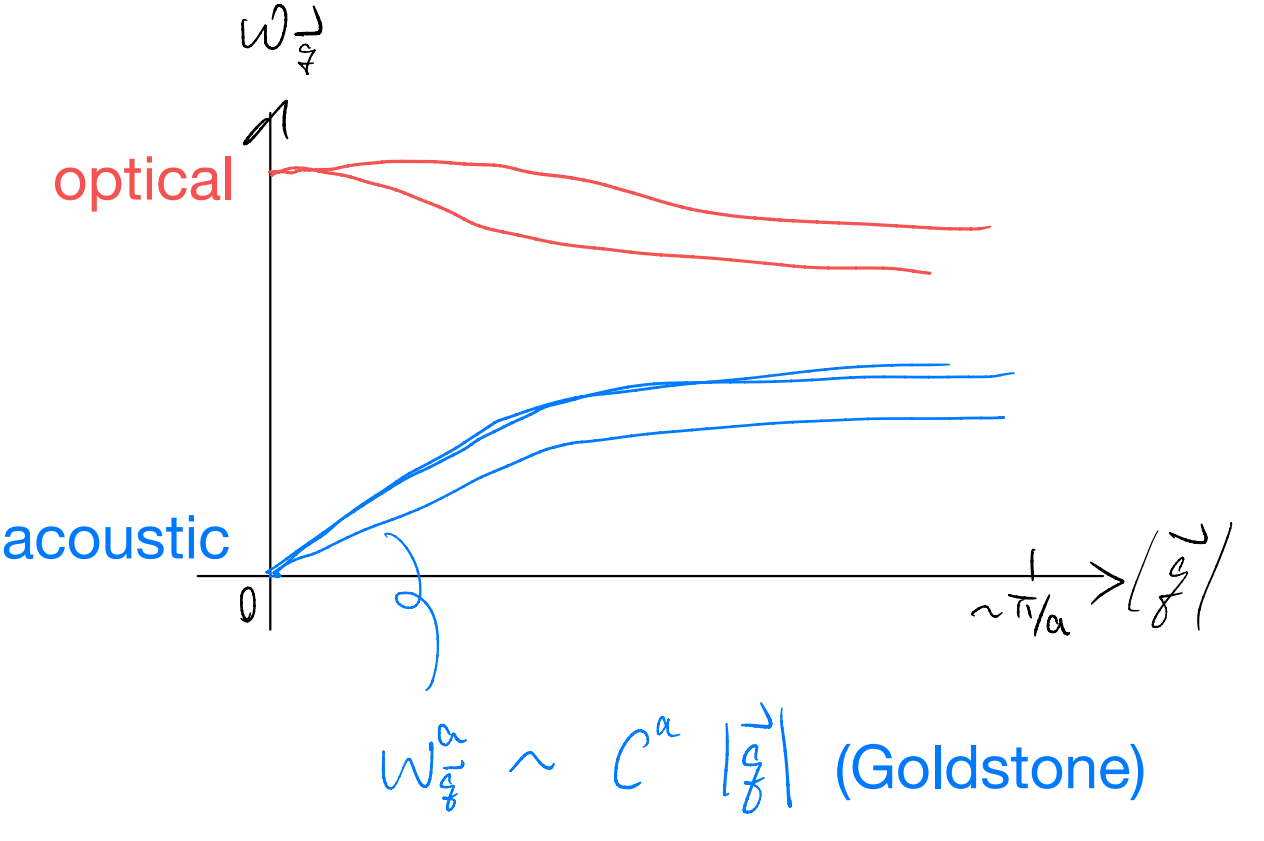
\includegraphics[width=\textwidth]{jupyterbook/data/fig/lec03-fig00.png}
    % \caption{caption environment}
    % \label{fig:00} %must after caption
\end{figure}

Goldstone modes: $\omega_{vec{q}}^\alpha\sim C^\alpha |\vec{q}|$

Anyway, we can finally write the phonon Hamiltonian as (CM abbretiate for Classical Mechanics)
\[ \hat{H}=\sum_{\alpha =1}^d{\frac{\hat{\Pi}_{\mathrm{CM}}^{\alpha 2}}{2M}}+\sum_{\alpha ,\vec{q}:q\ne 0}{\omega _{\vec{q}}^{\alpha}\left( \hat{a}_{\vec{q}}^{\alpha \dagger}\hat{a}_{\vec{q}}^{\alpha}+\frac{1}{2} \right)}\]
This isn't really any different from what we have without assuming translation symmetry! All we have gained is a more refined understanding on how the ``modes'' are organized with respect to the conserved crystal momentum.

Let's end this part by spending a bit of time thinking about the eigenstates, and then also what happens at finite temperature (as a quantum statistics mechanics review).

\section{Q stat mech review}

For simplicity, let's drop the CM motion piece. The phonon Hamiltonian is then
\[ \hat{H}=\sum_{\vec{q},\alpha}{\omega _{\vec{q}}^{\alpha}\left( \hat{a}_{\vec{q}}^{\alpha \dagger}\hat{a}_{\vec{q}}^{\alpha}+\frac{1}{2} \right)}\]
Each of the number operators $\hat{n}_{\vec{q}}=\hat{a}_{\vec{q}}^\dagger \hat{a}_{\vec{q}}$ commutes with the Hamiltonian, and so the eigenstates are simply labeled by them
\[ \hat{H}|\left\{ n_{\vec{q}}^{\alpha} \right\} \rangle =\sum_{\vec{q},\alpha}{\omega _{\vec{q}}^{\alpha}\left( n_{\vec{q}}^{\alpha}+\frac{1}{2} \right)}|\left\{ n_{\vec{q}}^{\alpha} \right\} \rangle \]
The constant $\omega_{\vec{q}}^\alpha/2$ in the Hamiltonian is problematic for two reasons
\begin{enumerate}
    \item It's shared by all states, but physical processes can only probe energy differences between states
    \item It scales with the number of atoms inside. If we wish to take a continuum limit, it diverges
\end{enumerate}
It is customary to simply drop that overall constant in the Hamiltonian. So far, we have focused on the eigenstates. At zero temperature, we can simply state that the system is in the lowest energy state. At finite temperatures, however, we expect states within an energy scale of $k_BT$ to be ``populated''. This is reflected in the density matrix.
\begin{gather*}
    \hat{\rho}=\frac{e^{-\beta \hat{H}}}{\mathcal{Z}}\\
    \mathcal{Z} =\mathrm{Tr}\left( e^{-\beta \hat{H}} \right) \\
    \beta =\frac{1}{k_BT}\\
    \mathrm{Tr}\left( \hat{\rho} \right) =1
\end{gather*}
Expectation value for a physical observable is then given by
\[ \left< \hat{A} \right> =\mathrm{Tr}\left( \hat{\rho}\hat{A} \right)  \]
For our free phonon problem, we know all the eigenstates and one can evaluate explicitly
\begin{align*}
    \mathcal{Z} \left( \beta \right) &=\mathrm{Tr}\left( e^{-\beta \hat{H}} \right) =\sum_{\left\{ n_{\vec{q}}^{\alpha} \right\}}{\langle \left\{ n_{\vec{q}}^{\alpha} \right\} |e^{-\beta \hat{H}}|\left\{ n_{\vec{q}}^{\alpha} \right\} \rangle}\\
    &=\sum_{\left\{ n_{\vec{q}}^{\alpha} \right\}}{\exp \left( -\beta \sum_{\vec{q},\alpha}{\omega _{\vec{q}}^{\alpha}n_{\vec{q}}^{\alpha}} \right)}\\
    &=\sum_{\left\{ n_{\vec{q}}^{\alpha} \right\}}{\prod_{\vec{q},\alpha}{\exp \left( -\beta \omega _{\vec{q}}^{\alpha}n_{\vec{q}}^{\alpha} \right)}}\\
    &=\prod_{\vec{q},\alpha}{\sum_{n_{\vec{q}}^{\alpha}=0}^{\infty}{\exp \left( -\beta \omega _{\vec{q}}^{\alpha}n_{\vec{q}}^{\alpha} \right)}}\\
    &=\prod_{\vec{q},\alpha}{\frac{1}{1-\exp \left( -\beta \omega _{\vec{q}}^{\alpha} \right)}}
\end{align*}
\[ \Rightarrow \ln \mathcal{Z} \left( \beta \right) =-\sum_{\vec{q},\alpha}{\ln \left( 1-e^{-\beta \omega _{\vec{q}}^{\alpha}} \right)}\]
To find, e.g., the energy expectation value we notice
\[ \left< H \right> =\frac{\mathrm{Tr}\left( \hat{H}\rho \right)}{\mathcal{Z}}=-\partial _{\beta}\ln \mathcal{Z} \left( \beta \right) \]
That's an awesome trick. What about computing some other expectation values? It's \emph{tempting} to imaging generalizing
\begin{gather*}
    \mathcal{Z} \left( \beta ,J \right) =\mathrm{Tr}\left( e^{-\beta \hat{H}+J\hat{O}} \right) \\
    \partial _J\ln \mathcal{Z} \left( \beta ,J \right) =\frac{\partial _J\mathrm{Tr}\left( e^{-\beta \hat{H}+J\hat{O}} \right)}{Z\left( \beta ,J \right)}\stackrel{?}{=}\frac{\mathrm{Tr}\left( \hat{O}e^{-\beta \hat{H}+J\hat{O}} \right)}{Z\left( \beta ,J \right)}\\
    \left. \partial _J\ln \mathcal{Z} \left( \beta ,J \right) \right|_{J=0}\stackrel{?}{=}\frac{\mathrm{Tr}\left( \hat{O}e^{-\beta \hat{H}} \right)}{Z\left( \beta ,J \right)}=\left< \hat{O} \right>
\end{gather*}
\emph{BUT} $\hat{H} \& \hat{O}$ may not commute! The manipulation above is faulty in general. Nevertheless, the spirit above is great. We just need a more sophisticated formalism to make it work. That requires time-ordering, generating functional, path integral etc. More later.

In any case, we have completely solved the free phonon problem, in the sense that for any observables we would want to compute, we have a way of doing so (by rotating to the decoupled QHO basis).

But let's pretend we are experimentalists. How do we even get to get to find the coupling coefficients etc in the first place? Without that, how do we find out the phonon frequencies etc? The natural approach is to perturb the system, and watches how it responds, e.g.,
\begin{figure}[ht]
    \centering
    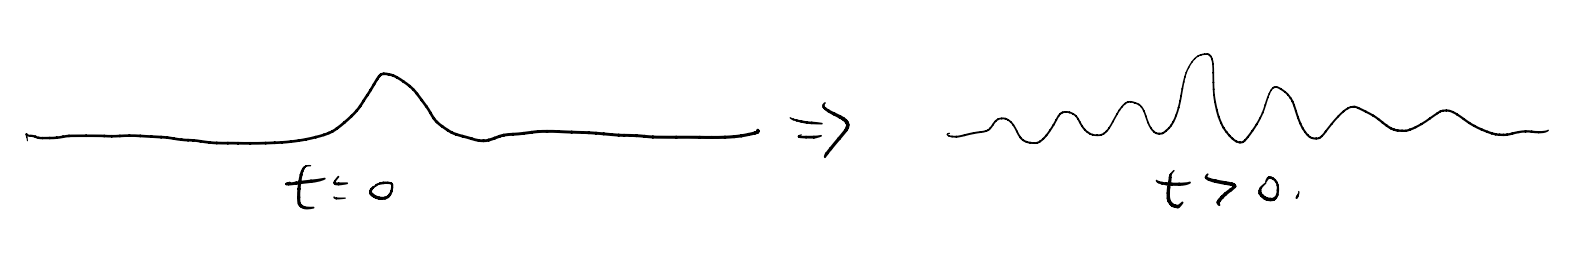
\includegraphics[width=\textwidth]{jupyterbook/data/fig/lec03-fig01.png}
    % \caption{caption environment}
    % \label{fig:00} %must after caption
\end{figure}
If you have a guitar string, you probe its frequency by plucking with you fingers, Too bad our fingers are too big for the microscopic crystal! Instead, we probe phonons with other tools, like photon, or more indirectly through electrons in the solid. E.g.
\begin{figure}[ht]
    \centering
    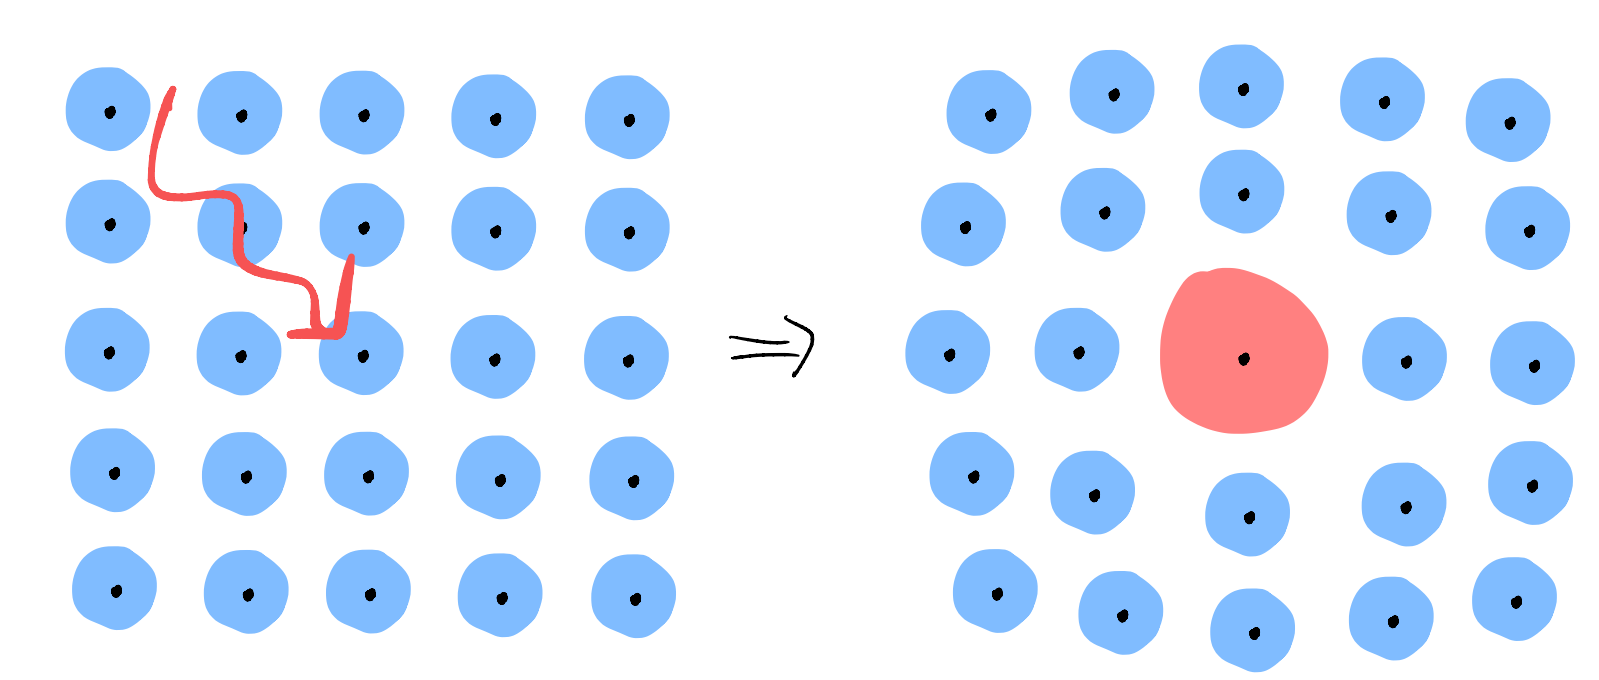
\includegraphics[width=\textwidth]{jupyterbook/data/fig/lec03-fig02.png}
    % \caption{caption environment}
    % \label{fig:00} %must after caption
\end{figure}
We generally expect the equilibrium position of the atoms to shift depending on the electronic state. So, we can use the electron as our ``phonon pick''!

To that end, let's now introduce the electron, a fermion.


\chapter{lec04 202200216}

topics

\begin{enumerate}
    \item particle statistics
    \item localized electrons
    \item Heisenberg picture
    \item Green's and spectral functions: a primer
\end{enumerate}

Goals

\begin{enumerate}
    \item relate particle statistics to (anti-)commutation of second quantized operators
    \item sharpening connection of Green's functions vs excitations
\end{enumerate}

Reminder: PS1 due coming Fri $1:30\text{pm}-\varepsilon$

\section{particle statistics}

We have mentioned on and off that phonon problem iis a bosonic one. Recall from QM that boson vs fermion is a question about particle exchange statistics. In the so-called ``first quantized'' wave function, a two-particle wave function dependss on two coordinate variables
\[ \Psi \left( x_1,x_2 \right) =\langle x_1,x_2|\Psi \rangle \]
``Particle statistics'' refers to what happen if we decide to relabel the two indistinguishable particles
\[ \Psi \left( x_1,x_2 \right) =\begin{cases}
	\Psi \left( x_2,x_1 \right) ;\quad \mathrm{boson}\\
	-\Psi \left( x_2,x_1 \right) ;\quad \mathrm{fermion}\\
\end{cases}\]
Generalization to an $N$-particle state is similar, noticing any permutation is a product of pair-wise exchanges. For our purpose, we just assert without any justification that one can relate the state with one boson at $x_1$ and one at $x_2$ can be identified with
\[ |x_1,x_2\rangle =\hat{b}_{x_1}^{\dagger}\hat{b}_{x_2}^{\dagger}|0\rangle \]
where $\hat{b}^\dagger$ is the creation operator we have written down countless time already from QHO. In essence, we associate to each point $x$ in space a QHO. The vacuum $|0\rangle$ is then the joint vacuum of all these QHO's.

Notes:
\begin{enumerate}
    \item but (if) space is continuous, then we have uncountably many QHO's even in a finite volume of space! That sounds sick. That is sick. But that's okay.
    \item We have implicitly promoted the single-particle wave function $\delta(x)$ to an operator $\hat{b}_x^\dagger$. That's why this is called ``second quantization''.
    \item implicitly, we have defined an object which maps space to quantum operators: $\vec{r}\to \hat{b}_x^\dagger$. Such maps are called ``fields''. (E.g., think about electric field $\vec{r}\to \vec{E_{\vec{r}}}$. Our fields here are quantum mechanical in that they do not have simple point-wise multiplication but instead cannonical commutation). Whence the name ``QFT''
\end{enumerate}

Now, back to particle statistics. We have, for bosons,
\[ \Psi _B\left( x_1,x_2 \right) =\langle 0|\hat{b}_{x_1}^{\dagger}\hat{b}_{x_2}^{\dagger}|0\rangle =\langle 0|\hat{b}_{x_2}^{\dagger}\hat{b}_{x_1}^{\dagger}|0\rangle =\Psi _B\left( x_2,x_1 \right) \]
So the exchange sign of $+1$ is really the commutation of among the creation(annihilation) operators. It is then natural to guess what should happen for fermions:
\[ \Psi _F\left( x_1,x_2 \right) =\langle 0|\hat{c}_{x_1}^{\dagger}\hat{c}_{x_2}^{\dagger}|0\rangle =-\langle 0|\hat{c}_{x_2}^{\dagger}\hat{c}_{x_1}^{\dagger}|0\rangle =\Psi _F\left( x_2,x_1 \right)  \]
This implies the fermionic creation and annihilation operators should satisfy cannonical anti-commutation relations. Let $\{\hat{A},\hat{B}\}=\hat{A}\hat{B}+\hat{B}\hat{A}$. For fermions
\[ \left\{ \hat{c}_x,\hat{c}_y \right\} =\left\{ \hat{c}_{x}^{\dagger},\hat{c}_{y}^{\dagger} \right\} =0 \]
\[ \left\{ \hat{c}_{x}^{\dagger},\hat{c}_y \right\} =\delta \left( x-y \right) \]
\[ \left\{ \hat{c}_x,\hat{c}_x \right\} =\left\{ \hat{c}_{x}^{\dagger},\hat{c}_{x}^{\dagger} \right\} =0\quad \Rightarrow \quad \hat{c}_{x}^{2}=\hat{c}_{x}^{\dagger 2}=0\]
Note: we take these as the practical definition for the ``second-quantized'' operators. One can also do it in the traditional way of making very explicit connections to the Hilbert space of symmetrized / anti-symmetrized wave functions. Schematically,
\begin{figure}[ht]
    \centering
    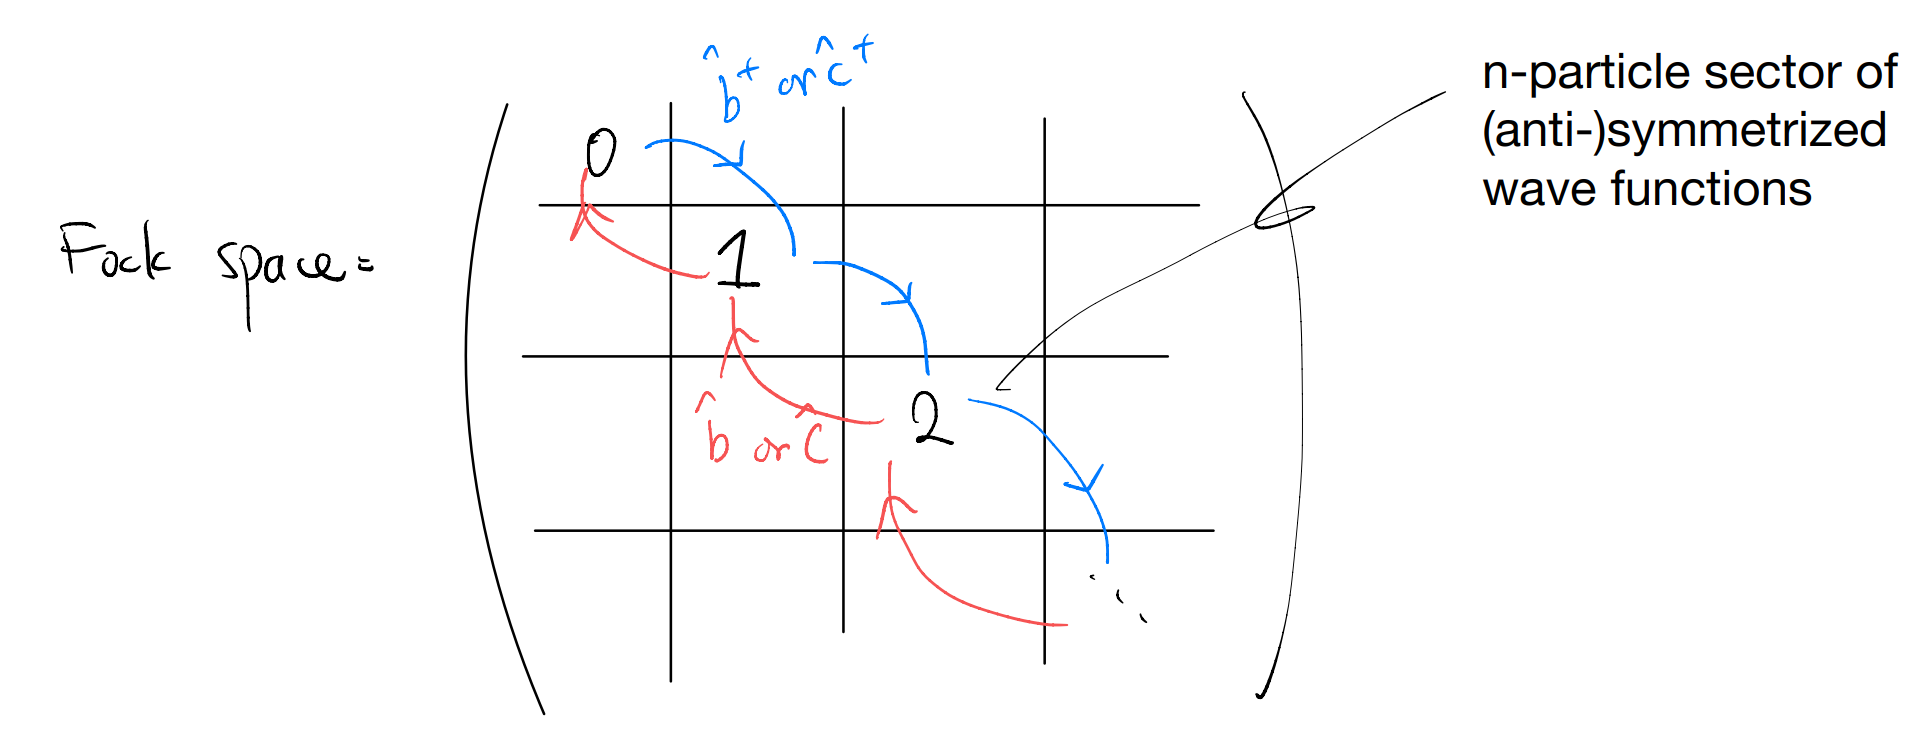
\includegraphics[width=\textwidth]{jupyterbook/data/fig/lec04-fig00.png}
    % \caption{caption environment}
    % \label{fig:00} %must after caption
\end{figure}
The ``first quantized'' description focus on each particle sector individually. The ``second quantized'' description focus on how to relate the different sectors. In particular, we have a natural relation between the ground state and a state in the $n$-particle sector. Consider putting $n$ particles (bosons or fermions) into $n$ ``orbitals'' $\phi_1,\phi_2,\cdots,\phi_n$
\[ \Phi _{x_1,x_2,\cdots ,x_n}^{\phi _1,\phi _2,\cdots ,\phi _n}\xrightarrow{\mathrm{sym}}\hat{b}_{\phi _1}^{\dagger}\hat{b}_{\phi _2}^{\dagger}\cdots \hat{b}_{\phi _n}^{\dagger}|0\rangle \quad \mathrm{bosons}\]
\[ \Phi _{x_1,x_2,\cdots ,x_n}^{\phi _1,\phi _2,\cdots ,\phi _n}\xrightarrow{\mathrm{anti}-\mathrm{sym}}\hat{c}_{\phi _1}^{\dagger}\hat{c}_{\phi _2}^{\dagger}\cdots \hat{c}_{\phi _n}^{\dagger}|0\rangle \quad \mathrm{fermions}\]
where we assume the ``orbitals'' are distinct and orthogonal. (i.e., we are considering a cannonical transformation on the defining modes of the system).

The above is rather schematic. In practice there are some factors of $\sqrt{n!}$ etc. if one wants to relate first and second quantization. We won't cover that here (usually covered in advanced QM), see e.g. Coleman Chapter-3 for more details.

Final note: so is QHO bosonic?

\emph{It depends}. IF you have exactly one particle, there is no exchange and hense no statistics. If you have multple particles, then the statistics is an ``intrinsic'' aspect of the problem in the sense that it defines the many-body Hilbert space, whereas being a QHO is ``kinematic'' in the sense that it's just characterizing the Hamiltonian acting on the Hilbert space. E.g.,
\begin{enumerate}
    \item Phonons: the momenta and displacements of different atoms commute, so we have a bosonic problem to start with. In the ``harmonic approximation'' we have a collection of coupled QHO
    \item Electronic quantum Hall: we have fermions to start with, but the B-field enters the single particle problem as a spatially varying gauge field. That also leads to the QHO Hamiltonian for the single particle problem. But now the raising / lowering operators act between different \emph{fermionic} modes that could be empty or filled
\end{enumerate}

P.S. We can certainly have bosonic operators in a fermionic Hilbert space: combining an even number of fermionic operators leads to bosonic ones. For those of you have prefer a math-oriented language, the operator algebra is $Z_2$-graded and we have even=bosonic and odd=fermionic.

P.P.S. We can even have effectively fermionic operators in a bosonic Hilbert space. That's the wonder of topological order...

\section{Localized electrons}

Let us now consider our very first electronic problem. Consider as a warm-up an electronic Hamiltonian
\begin{align*}
    \hat{H}=&\varepsilon \left( \hat{c}_{\uparrow}^{\dagger}\hat{c}_{\downarrow}+\hat{c}_{\downarrow}^{\dagger}\hat{c}_{\uparrow} \right) \quad \mathrm{many body}\\
    &=\left( \hat{c}_{\uparrow}^{\dagger},\hat{c}_{\downarrow}^{\dagger} \right) \left( \begin{matrix}
        0&		\varepsilon\\
        \varepsilon&		0\\
    \end{matrix} \right) \left( \hat{c}_{\uparrow},\hat{c}_{\downarrow} \right) \quad \mathrm{single particle}\\
\end{align*}
Let's consider writing out the matrix elements in the Fock space
\[ \hat{H}|0\rangle =\varepsilon \left( \hat{c}_{\uparrow}^{\dagger}\hat{c}_{\downarrow}+\hat{c}_{\downarrow}^{\dagger}\hat{c}_{\uparrow} \right) |0\rangle =0\]
\begin{align*}
    \hat{H}\hat{c}_{\uparrow}^{\dagger}|0\rangle &=\varepsilon \left( \hat{c}_{\uparrow}^{\dagger}\hat{c}_{\downarrow}+\hat{c}_{\downarrow}^{\dagger}\hat{c}_{\uparrow} \right) \hat{c}_{\uparrow}^{\dagger}|0\rangle \\
    &=\varepsilon \left( \hat{c}_{\uparrow}^{\dagger}\hat{c}_{\downarrow}\hat{c}_{\uparrow}^{\dagger}+\hat{c}_{\downarrow}^{\dagger}\hat{c}_{\uparrow}\hat{c}_{\uparrow}^{\dagger} \right) |0\rangle \\
    &=\varepsilon \left( -\hat{c}_{\uparrow}^{\dagger}\hat{c}_{\uparrow}^{\dagger}\hat{c}_{\downarrow}+\hat{c}_{\downarrow}^{\dagger}\left( 1-\hat{c}_{\uparrow}^{\dagger}\hat{c}_{\uparrow} \right) \right) |0\rangle \\
    &=\varepsilon \left( 0+\hat{c}_{\downarrow}^{\dagger}-\hat{c}_{\downarrow}^{\dagger}\hat{c}_{\uparrow}^{\dagger}\hat{c}_{\uparrow} \right) |0\rangle \\
    &=\varepsilon \left( 0+\hat{c}_{\downarrow}^{\dagger}-0 \right) |0\rangle \\
    &=\varepsilon \hat{c}_{\downarrow}^{\dagger}|0\rangle
\end{align*}
\[ \hat{H}\hat{c}_{\downarrow}^{\dagger}|0\rangle =\varepsilon \left( \hat{c}_{\uparrow}^{\dagger}\hat{c}_{\downarrow}+\hat{c}_{\downarrow}^{\dagger}\hat{c}_{\uparrow} \right) \hat{c}_{\downarrow}^{\dagger}|0\rangle =\varepsilon \hat{c}_{\uparrow}^{\dagger}|0\rangle \]
\[ \hat{H}\hat{c}_{\uparrow}^{\dagger}\hat{c}_{\downarrow}^{\dagger}|0\rangle =\varepsilon \left( \hat{c}_{\uparrow}^{\dagger}\hat{c}_{\downarrow}+\hat{c}_{\downarrow}^{\dagger}\hat{c}_{\uparrow} \right) \hat{c}_{\uparrow}^{\dagger}\hat{c}_{\downarrow}^{\dagger}|0\rangle =0 \]
\[ \hat{H}=\left( \begin{matrix}
	0&		0&		0&		0\\
	0&		0&		\varepsilon&		0\\
	0&		\varepsilon&		0&		0\\
	0&		0&		0&		0\\
\end{matrix} \right) \]
% TODO kbordermatrix https://tex.stackexchange.com/a/59732
in the basis $\left\{ |0\rangle ,\hat{c}_{\uparrow}^{\dagger}|0\rangle ,\hat{c}_{\downarrow}^{\dagger}|0\rangle ,\hat{c}_{\uparrow}^{\dagger}\hat{c}_{\downarrow}^{\dagger}|0\rangle \right\}$ ($\left\{ \hat{c}_{\uparrow}^{\dagger}|0\rangle ,\hat{c}_{\downarrow}^{\dagger}|0\rangle \right\}$ is single-particle basis). We know the single-particle eigenstates are
\[ \varepsilon \left( \begin{matrix}
	0&		1\\
	1&		0\\
\end{matrix} \right) \left( \begin{array}{c}
	1\\
	\pm 1\\
\end{array} \right) =\pm \varepsilon \left( \begin{array}{c}
	1\\
	\pm 1\\
\end{array} \right)\]
It is natural to ``rotate'' in the eigenbasis
\[ \hat{c}_{+}^{\dagger}=\frac{1}{\sqrt{2}}\left( \hat{c}_{\uparrow}^{\dagger}+\hat{c}_{\downarrow}^{\dagger} \right) ,\quad \hat{c}_{-}^{\dagger}=\frac{1}{\sqrt{2}}\left( \hat{c}_{\uparrow}^{\dagger}-\hat{c}_{\downarrow}^{\dagger} \right) \]
we may check
\[ \begin{cases}
	\left\{ \hat{c}_{\pm}^{\dagger},\hat{c}_{\pm} \right\} =\frac{1}{2}\left\{ \hat{c}_{\uparrow}^{\dagger}\pm \hat{c}_{\downarrow}^{\dagger},\hat{c}_{\uparrow}\pm \hat{c}_{\downarrow} \right\} =\frac{1}{2}\left( 1\pm 0\pm 0+1 \right) =1\\
	\left\{ \hat{c}_{+}^{\dagger},\hat{c}_- \right\} =\frac{1}{2}\left\{ \hat{c}_{\uparrow}^{\dagger}+\hat{c}_{\downarrow}^{\dagger},\hat{c}_{\uparrow}-\hat{c}_{\downarrow} \right\} =\frac{1}{2}\left( 1+0-0-1 \right) =0\\
\end{cases}\]
\[ \Rightarrow \begin{cases}
	\left\{ \hat{c}_{\alpha}^{\dagger},\hat{c}_{\beta} \right\} =\delta _{\alpha \beta}\\
	\left\{ \hat{c}_{\alpha}^{\dagger},\hat{c}_{\beta}^{\dagger} \right\} =\left\{ \hat{c}_{\alpha},\hat{c}_{\beta} \right\} =0\\
\end{cases}\]
Using which we have
\[ \hat{H}=\varepsilon \hat{c}_{+}^{\dagger}\hat{c}_+-\varepsilon \hat{c}_{-}^{\dagger}\hat{c}_-\]
We can schematically draw the spectrum as ($\varepsilon>0$)
\begin{figure}[ht]
    \centering
    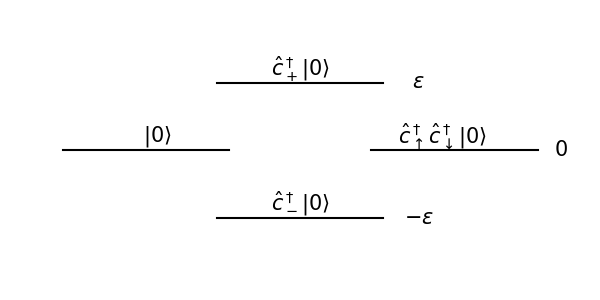
\includegraphics[width=\textwidth]{jupyterbook/data/fig/lec04-fig01.png}
    % \caption{caption environment}
    % \label{fig:00} %must after caption
\end{figure}

Side note: The calculation above can be readily generalized. Consider some Hamiltonian defined over $N$ fermionic modes:
\[ \hat{H}=\sum_{\alpha ,\beta =1}^N{\hat{c}_{\alpha}^{\dagger}h_{\alpha \beta}\hat{c}_{\beta}}\]
Here, $h$ is a Hermitian matrix and can be diagonalized by a unitary
\[ h_{\alpha \beta}=\sum_i{U_{\alpha i}\varepsilon _i\left( U^{\dagger} \right) _{i\beta}}\]
\begin{align*}
    \hat{H}&=\sum_i{\left( \sum_{\alpha}{\hat{c}_{\alpha}^{\dagger}}U_{\alpha i} \right) \varepsilon _i\left( \sum_{\beta}{\left( U^{\dagger} \right) _{i\beta}\hat{c}_{\beta}} \right)}\\
    &=\sum_i{\varepsilon _i\hat{c}_{i}^{\dagger}\hat{c}_i}\quad \mathrm{cannonical transformation}
\end{align*}
(c.f. the phonon discusion)

Back to the two mode problem: this is again an exactly solved problem, which is in a way similar to the QHO / free phonon. We know all the eigenstates and eigen-energies. Yet, it is natural to ask how we can probe the ``physics'' of the system. Suppose we start with the ground state ($t>0$):
\[ |\Omega \rangle =\hat{c}_{-}^{\dagger}|0\rangle =\frac{1}{\sqrt{2}}\left( \hat{c}_{\uparrow}^{\dagger}-\hat{c}_{\downarrow}^{\dagger} \right) |0\rangle \]
Recall our discussion on propagator / correlation functions / Green's functions. Let us compare
\begin{enumerate}
    \item create an up electron: $\hat{c}_\uparrow^\dagger$
    \item evolution for time $t$: $e^{-i\hat{H}t}$
\end{enumerate}
\[ e^{-i\hat{H}t}\hat{c}_{\uparrow}^{\dagger}|\Omega \rangle \quad \mathrm{vs}\quad \hat{c}_{\uparrow}^{\dagger}e^{-i\hat{H}t}|\Omega \rangle \]
\[ \quad G_{\uparrow \uparrow}\left( t \right) =-i\langle \Omega |e^{i\hat{H}t}\hat{c}_{\uparrow}e^{-i\hat{H}t}\hat{c}_{\uparrow}^{\dagger}|\Omega \rangle \]
where $e^{i\hat{H}t}\hat{c}_{\uparrow}e^{-i\hat{H}t}$ iss the conjugate action of time evolution on an operator. We clained
\begin{enumerate}
    \item Such functions contains important dynamical info about the system
    \item It is natural to interpret it as a specific kind of correlation function
\end{enumerate}
Let us now introduce these ideas more systematically

Heisenberg picture

So far, we have introduced time evolution of a quantum system through the evolution operator $\hat{U}=e^{-i\hat{H}t}$, which satisfies
\[ i\partial _t\hat{U}=\hat{H}\hat{U}\]
Implicitly, we know that if a state satisfies the Schrodinger equation
\[ i\partial _t|\Psi \left( t \right) \rangle =\hat{H}|\Psi \left( t \right) \rangle \]
then its time evolution can be expressed simply as
\[ |\Psi \left( t \right) \rangle =\hat{U}|\Psi \left( 0 \right) \rangle =e^{-i\hat{H}t}|\Psi \left( 0 \right) \rangle \]
\[ i\partial _t|\Psi \left( t \right) \rangle =i\partial _t\left( \hat{U}|\Psi \left( 0 \right) \rangle \right) =\left( i\partial _t\hat{U} \right) |\Psi \left( 0 \right) \rangle =\hat{H}\left( \hat{U}|\Psi \left( 0 \right) \rangle \right) =\hat{H}|\Psi \left( t \right) \rangle \]
Now imagine computing some observables as the state evolves
\[ A\left( t \right) =\langle \Psi \left( t \right) |\hat{A}|\Psi \left( t \right) \rangle =\langle \Psi \left( 0 \right) |\hat{U}^{\dagger}\hat{A}\hat{U}|\Psi \left( 0 \right) \rangle \]
It's simply a mater of interpretation to say that the operator is evolving $\hat{A}\rightarrow \hat{U}^{\dagger}\hat{A}\hat{U}$, and we compute its expectation value with resepct to a fixed state $|\Psi\rangle(0)$. This perspective is called the ``Heisenberg picture''.
\[ \mathrm{Schrodinger}\begin{cases}
	|\Psi \left( 0 \right) \rangle _S\rightarrow |\Psi \left( t \right) \rangle _S=\hat{U}|\Psi \left( 0 \right) \rangle _S\\
	\hat{A}_S\rightarrow \hat{A}_S\\
\end{cases}\]
\[ \mathrm{Heisenberg}\begin{cases}
	|\Psi \rangle _H\rightarrow |\Psi \rangle _H\\
	\hat{A}_H\left( 0 \right) \rightarrow \hat{A}_H\left( t \right) =\hat{U}^{\dagger}\hat{A}_H\left( 0 \right) \hat{U}\\
\end{cases}\]
Here we assume the operator is time-independent in the Schrodinger picture. We can also check explicitly what is the equation governing the time evolution of Heisenberg-picture operators:
\begin{align*}
    i\partial _t\hat{A}_H\left( t \right) &=i\partial _t\left( \hat{U}^{\dagger}\hat{A}_H\left( 0 \right) \hat{U} \right) \\
    &=-\hat{H}\hat{A}_H\left( t \right) +\hat{A}_H\left( t \right) \hat{H}\\
    &=\left[ \hat{A}_H\left( t \right) ,\hat{H} \right]
\end{align*}
In fact, nothing in the check above demands that we use the actual Hamiltonian! One can imagine picking a ``convenient'' part of the actual Hamiltonian in defining the dynamics of the operators. Correspondingly, however, the state vectors are \emph{not} static since we are not using the actual Hamiltonian. In this hybrid picture, both the operators and the state evolve. This is called the ``interaction picture''; more later.

Note: for those of you who know quantum optics, think about rotating wave approximation.

\section{One-particle Green's function: a first example}

In the following, we keep the subscript $S$ vs $H$ implicit. Whenever we write a time dependence for a noperator, it is understood that we are in the Heisenberg picture.

Back to our example. Recall we were compairing
\[ \hat{c}_{\uparrow}^{\dagger}e^{-i\hat{H}t}|\Omega \rangle \quad \mathrm{vs}\quad e^{-i\hat{H}t}\hat{c}_{\uparrow}^{\dagger}|\Omega \rangle \]
where
\[ \hat{H}=\varepsilon \left( \hat{c}_{\uparrow}^{\dagger}\hat{c}_{\downarrow}+\hat{c}_{\downarrow}^{\dagger}\hat{c}_{\uparrow} \right) \]
\[ |\Omega \rangle =\frac{1}{\sqrt{2}}\left( \hat{c}_{\uparrow}^{\dagger}-\hat{c}_{\downarrow}^{\dagger} \right) |0\rangle \]
In Heisenberg picture, we have defined
\begin{align*}
    G_{\uparrow \uparrow}\left( t \right) &=-i\langle \Omega |e^{i\hat{H}t}\hat{c}_{\uparrow}e^{-i\hat{H}t}\hat{c}_{\uparrow}^{\dagger}|\Omega \rangle \\
    &=-i\langle \Omega |\hat{c}_{\uparrow}\left( t \right) \hat{c}_{\uparrow}^{\dagger}\left( 0 \right) |\Omega \rangle
\end{align*}
which can be interpreted as a (quantum) auto-correlation function: we create an electron at time $t=0$, and then annihilate it at time $t$. We are measureing correlation across time. Yet, this is \emph{NOT} by itself a physical observable! We cannot understand it as the expectation vlue of some Hermitian operator. Nevertheless, ``unphysical'' expressions of such form provides the basis for computing actual observables. As one first check, let us investigate how $G(t)$ reflects the energy scale of the problem. Noticing
\[ \hat{H}=\varepsilon \hat{c}_{+}^{\dagger}\hat{c}_+-\varepsilon \hat{c}_{-}^{\dagger}\hat{c}_-\]
\[ \hat{c}_{\pm}^{\dagger}=\frac{1}{\sqrt{2}}\left( \hat{c}_{\uparrow}^{\dagger}\pm \hat{c}_{\downarrow}^{\dagger} \right) \]
we first note that time evolution for $\hat{c}_{\pm}^\dagger$ is simple. In the Heisenberg picture,
\begin{align*}
    i\partial _t\left( {\color{blue} \hat{c}_{\pm}^{\dagger}\left( t \right) } \right) &=\left[ {\color{blue} \hat{c}_{\pm}^{\dagger}\left( t \right) },\hat{H} \right] \\
    &=\hat{U}^{\dagger}\left[ {\color{red} \hat{c}_{\pm}^{\dagger}},\pm \varepsilon {\color{red} \hat{c}_{\pm}^{\dagger}\hat{c}_{\pm}} \right] \hat{U}\\
    &=\hat{U}^{\dagger}\left( \pm \varepsilon {\color{red} \hat{c}_{\pm}^{\dagger}} \right) \left[ {\color{red} \hat{c}_{\pm}^{\dagger}},{\color{red} \hat{c}_{\pm}} \right] \hat{U}\\
    &=\hat{U}^{\dagger}\left( \pm \varepsilon {\color{red} \hat{c}_{\pm}^{\dagger}} \right) \left( 2{\color{red} \hat{c}_{\pm}^{\dagger}\hat{c}_{\pm}}-1 \right) \hat{U}\\
    &=\mp \varepsilon {\color{blue} \hat{c}_{\pm}^{\dagger}\left( t \right) }
\end{align*}
\[ {\color{blue} \hat{c}_{\pm}^{\dagger}\left( t \right) }={\color{blue} \hat{c}_{\pm}^{\dagger}\left( 0 \right) }e^{\pm i\varepsilon t}\]
With the blue symbols denoting Heisenberg picture and the red symbols Schrodinger picture. Noticing $\hat{c}_{\uparrow}^{\dagger}\left( t \right) =\frac{1}{\sqrt{2}}\left( \hat{c}_{+}^{\dagger}\left( t \right) +\hat{c}_{-}^{\dagger}\left( t \right) \right)$,
\begin{align*}
    G_{\uparrow \uparrow}\left( t \right) &=-i\langle \Omega |\hat{c}_{\uparrow}\left( t \right) \hat{c}_{\uparrow}^{\dagger}\left( 0 \right) |\Omega \rangle \\
    &=-\frac{i}{2}\langle \Omega |\left( \hat{c}_+\left( t \right) +\hat{c}_-\left( t \right) \right) \left( \hat{c}_{+}^{\dagger}\left( 0 \right) +\hat{c}_{-}^{\dagger}\left( 0 \right) \right) |\Omega \rangle \\
    &=-\frac{i}{2}\langle 0|\hat{c}_-\left( \hat{c}_+e^{-i\varepsilon t}+\hat{c}_-e^{i\varepsilon t} \right) \left( \hat{c}_{+}^{\dagger}+\hat{c}_{-}^{\dagger} \right) \hat{c}_{-}^{\dagger}|0\rangle \\
    &=-\frac{i}{2}\langle 0|\hat{c}_-\hat{c}_+e^{-i\varepsilon t}\hat{c}_{+}^{\dagger}\hat{c}_{-}^{\dagger}|0\rangle \\
    &=-\frac{i}{2}e^{-i\varepsilon t}\langle 0|\left( 1-\hat{c}_{+}^{\dagger}\hat{c}_+ \right) \left( 1-\hat{c}_{-}^{\dagger}\hat{c}_- \right) |0\rangle \\
    &=-\frac{i}{2}e^{-i\varepsilon t}
\end{align*}
How to interpret this?
\begin{figure}[h]
    \centering
    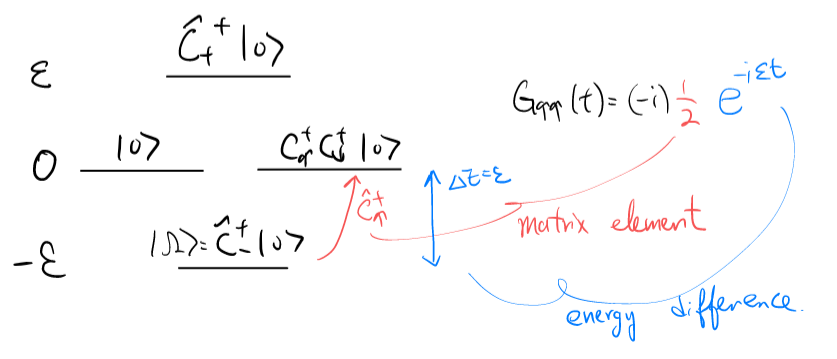
\includegraphics[width=\textwidth]{jupyterbook/data/fig/lec04-fig02.png}
    % \caption{caption environment}
    % \label{fig:00} %must after caption
\end{figure}

\section{One-particle Green's function and spectral Lehmann representation}

Our ``single-site'' example is designed to be simple (simple enough to solve everything exactly). Interestingly, the physical picture derived from above is actually very general, as we will see now.

Suppose we have an electronic problem with some many-body Hamiltonian $\hat{H}$ and the ground state $|\Omega\rangle$. We consider the one-particle Green's function as defined above:
\begin{align*}
    G_{\alpha \alpha}\left( t \right) &=-i\langle \Omega |\hat{c}_{\alpha}\left( t \right) \hat{c}_{\alpha}^{\dagger}\left( 0 \right) |\Omega \rangle _H\\
    &=-i\langle \Omega |e^{i\hat{H}t}\hat{c}_{\alpha}e^{-i\hat{H}t}\hat{c}_{\alpha}^{\dagger}|\Omega \rangle _S
\end{align*}
where we use one subscript to denote if the expression is understood in the Heisenberg or Schrodinger picture.

To probe the dynamics, it is natural to go to the eigenbasis of the Hamiltonian. We insert a complete set of basis
\begin{align*}
    G_{\alpha \alpha}\left( t \right) &=-i\sum_n{e^{iE_{\Omega}t}\langle \Omega |\hat{c}_{\alpha}|n\rangle _Se^{-iE_nt}\langle n|\hat{c}_{\alpha}^{\dagger}|\Omega \rangle _S}\\
    &=-i\sum_n{\left| \langle n|\hat{c}_{\alpha}^{\dagger}|\Omega \rangle _S \right|^2e^{-i\left( E_n-E_{\Omega} \right) t}}
\end{align*}
where $\langle n|\hat{c}_{\alpha}^{\dagger}|\Omega \rangle _S$ is the matrix element and $e^{-i\left( E_n-E_{\Omega} \right) t}$ is the energy difference. This is practically identical to what we had, but we now know neither the matrix element nor the excitation energy (i.e., energy difference from the ground state)!

Importantly, the many-body spectrum is dense! Remember the number of quantum states scales exponentially with the system size $\text{dim}(\mathcal{H})\sim 2^V$.


\chapter{lec05 202200218}

Topics

\begin{enumerate}
    \item Spectral function
    \item (Thought) experiment on spectroscopy
    \item The zoo of Green's functions
    \item Impurity-phonon coupling
\end{enumerate}

Goals

\begin{enumerate}
    \item developing intuition about Green's and spectral functions
    \item Appreciating how they relate to physical problems
    \item Applying the techniques to a less trivial and physically relevant problem
\end{enumerate}

\section{Spectral function}

Last time, we were considering a ``one-particle'' Green's function in a general quantum many-body problem
\begin{align*}
    G_{\alpha \alpha}\left( t \right) &=\left( -i \right) \langle \Omega |\hat{c}_{\alpha}\left( t \right) \hat{c}_{\alpha}^{\dagger}\left( 0 \right) |\Omega \rangle _H\\
    &=\left( -i \right) \sum_n{\left| \langle n|\hat{c}_{\alpha}^{\dagger}|\Omega \rangle \right|^2e^{-i\left( E_n-E_{\Omega} \right) t}}
\end{align*}
\[ \Delta E_n=\left( E_n-E_{\Omega} \right) \ge 0\]
where $n$ labels the complete (but unknown) eigenstates of the Hamiltonian. We will continue analyzing how much information we can gain from considering such expressions. We would want to understand the excitation energies. However, in general it is hopeless to try to resolve each of the frequencies. Instead, we should think of a distribution of frequencies, and prominent features will be ``peaks'' with some widths. This can be done systematically by Fourier transform with respect to time $t$
\begin{align*}
    G_{\alpha \alpha}\left( \omega \right) &\stackrel{?}{=} \int_{-\infty}^{\infty}{dtG_{\alpha \alpha}\left( t \right) e^{i\omega t}}\\
    &=-i\sum_n{\int_{-\infty}^{\infty}{\left| \langle n|\hat{c}_{\alpha}^{\dagger}|\Omega \rangle \right|^2e^{i\left( \omega -\Delta E_n \right) t}}}
\end{align*}
But there's a serious issue: the integrand is oscillating as we attempt to Fourier transform with $t\to \pm\infty$. Clearly this is an artifact of our mathematical treatment: we don't know if our universe existed or will exist all the way to $t=\pm\infty$!

Here, let us do two things to circumvent the problem
\begin{enumerate}
    \item In our thought experiment, we always let the system evolve forward in time when we evaluate the auto-correlation. In other words, we restrict ourselves to $t\geq 0$
    \item we won't be able to access $t\to +\infty$ anyway. Let's ``damp'' the contribution by adding a convergence factor $e^{-\eta t}$ to the integrand, taking $\eta\to 0^+$
\end{enumerate}
\begin{align*}
    G_{\alpha \alpha}\left( \omega \right) &=\lim_{\eta \rightarrow 0^+} \left( -i \right) \int_0^{\infty}{dtG_{\alpha \alpha}\left( t \right) e^{i\omega t}e^{-\eta t}}\\
    &=\lim_{\eta \rightarrow 0^+} \left( -i \right) \sum_n{\left| \langle n|\hat{c}_{\alpha}^{\dagger}|\Omega \rangle \right|^2\int_0^{\infty}{e^{i\left( \omega -\Delta E_n+i\eta \right) t}}}\\
    &=\lim_{\eta \rightarrow 0^+} \sum_n{\frac{\left( -i \right) \left| \langle n|\hat{c}_{\alpha}^{\dagger}|\Omega \rangle \right|^2}{i\left( \omega -\Delta E_n+i\eta \right)}\left( e^{-\eta \left( +\infty \right)}-1 \right)}\\
    &=\lim_{\eta \rightarrow 0^+} \sum_n{\frac{\left| \langle n|\hat{c}_{\alpha}^{\dagger}|\Omega \rangle \right|^2}{\omega -\Delta E_n+i\eta}}
\end{align*}
Notes:
\begin{enumerate}
    \item this explains the convention of attaching $(-i)$ to the definition of $G_{\alpha\alpha}(t)$
    \item $G_{\alpha\alpha}(\omega)$ as a function over $\omega$ has a (dense) series of poles at $\omega=\Delta E_n-i\eta$
\end{enumerate}

\begin{figure}[ht]
    \centering
    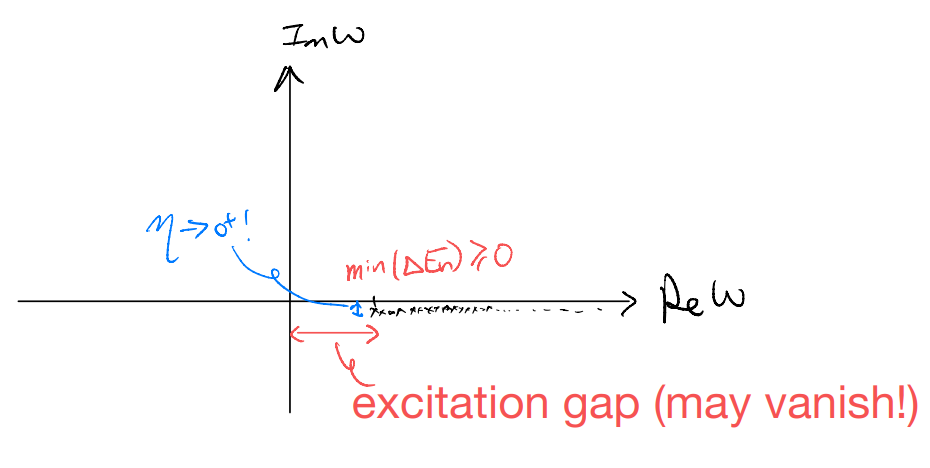
\includegraphics[width=\textwidth]{jupyterbook/data/fig/lec05-fig00.png}
\end{figure}

But this is still not something we can measure directly! The matrix element $\left| \langle n|\hat{c}_{\alpha}^{\dagger}|\Omega \rangle \right|^2$ is physical: it corresponds to the transition probability of the ground state to some excited state when we add an electron to it. But energy information is hidden in the location of the poles which we displaced below the real line by a sleight of hand. We now claim that, in fact one can identify a ``spectral function'', closely related to actual experiments, from the frequency-space Green's function:
\[ A_{\alpha \alpha}\left( \omega \right) =\frac{-1}{\pi}\mathrm{Im}\left[ G_{\alpha \alpha}\left( \omega \right) \right] =\sum_n{\left| \langle n|\hat{c}_{\alpha}^{\dagger}|\Omega \rangle \right|^2\delta \left( \omega -\Delta E_n \right)}\]
where $\left| \langle n|\hat{c}_{\alpha}^{\dagger}|\Omega \rangle \right|^2$ is the matrix element and $\delta \left( \omega -\Delta E_n \right)$ is the density of states. We will give a ``lousy'' derivation here first; will revisit later. Noticing
\[ \frac{1}{x+i\eta}=\frac{x}{x^2+\eta ^2}-i\frac{\eta}{x^2+\eta ^2}\]
We will handle the real part later. The imaginary part looks like

\begin{figure}[ht]
    \centering
    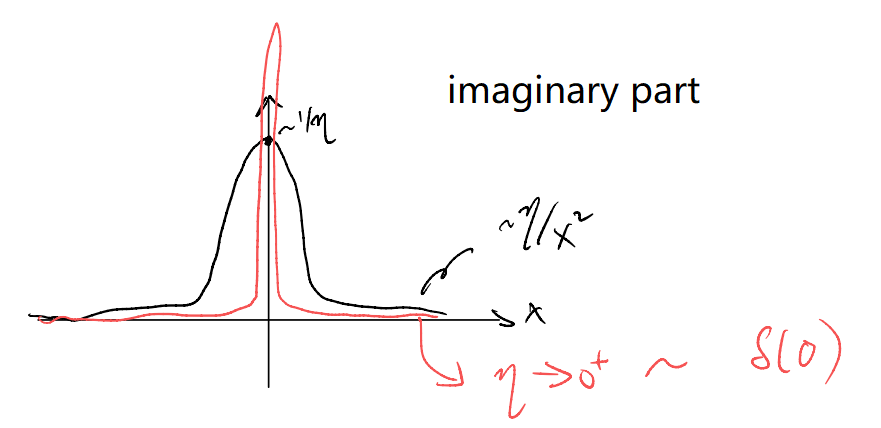
\includegraphics[width=\textwidth]{jupyterbook/data/fig/lec05-fig01.png}
\end{figure}

Normalization:
\[ \int_{-\infty}^{\infty}{dx\frac{\eta}{x^2+\eta ^2}}=\pi \]
\[ \Rightarrow \lim_{\eta \rightarrow 0^+} \mathrm{Im}\left[ \frac{1}{x+i\eta} \right] =-\pi \delta \left( 0 \right) \]
This gives
\begin{align*}
    A_{\alpha \alpha}\left( \omega \right) &=\frac{-1}{\pi}\lim_{\eta \rightarrow 0^+} \mathrm{Im}\sum_n{\frac{\left| \langle n|\hat{c}_{\alpha}^{\dagger}|\Omega \rangle \right|^2}{\omega -\Delta E_n+i\eta}}\\
    &=\sum_n{\left| \langle n|\hat{c}_{\alpha}^{\dagger}|\Omega \rangle \right|^2\delta \left( \omega -\Delta E_n \right)}
\end{align*}
where $\left| \langle n|\hat{c}_{\alpha}^{\dagger}|\Omega \rangle \right|^2\delta(\omega-\Delta E_n)$ is the probability of finding the system in the $|n\rangle$ eigenstate when we add an electron $\hat{c}_{\alpha}^{\dagger}$ to the ground state $|\Omega\rangle$ with energy $\omega$ matching $\Delta E_n$. How can we measure a quantity like that?

STM: trying to add electrons to the sample (approx. in the ground state at low temperature)

\begin{figure}[ht]
    \centering
    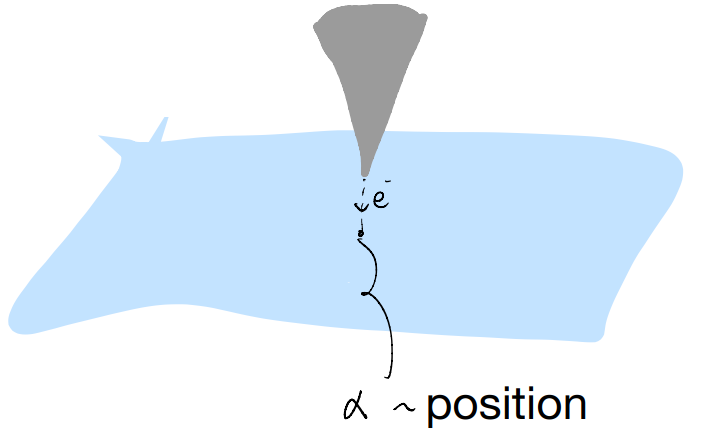
\includegraphics[width=\textwidth]{jupyterbook/data/fig/lec05-fig02.png}
\end{figure}

But STM doesn't only try to add electrons! The tip also tries to ``pull'' electrons out of the sample, i.e., remove electron from the ground state, Similarly for ARPES

\begin{figure}[ht]
    \centering
    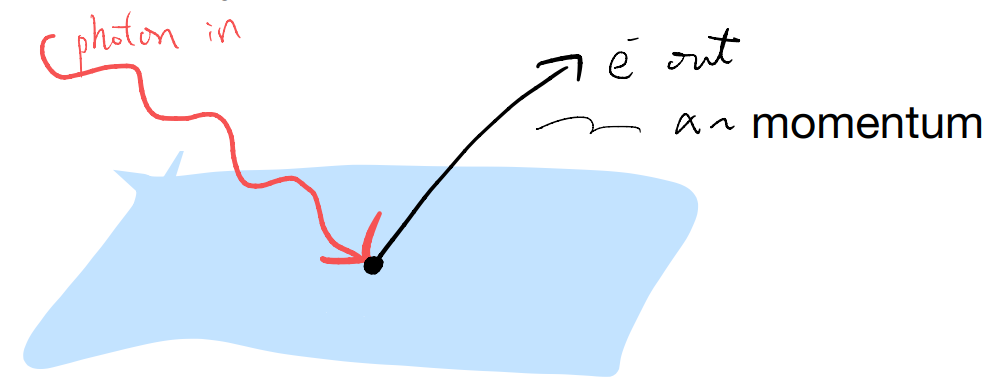
\includegraphics[width=\textwidth]{jupyterbook/data/fig/lec05-fig03.png}
\end{figure}

Clearly, there are many more things one can do. We are only starting to see the tip of the iceberg.

\section{Ground state deduction: a thought experiment}

Now, let's imagine plotting this spectral function. First, let us revert to our simple ``single-orbital'' example
\[ \hat{H}=\varepsilon \left( \hat{c}_{\uparrow}^{\dagger}\hat{c}_{\downarrow}+\hat{c}_{\downarrow}^{\dagger}\hat{c}_{\uparrow} \right) \]
\[ G_{\uparrow \uparrow}\left( t \right) =-i\frac{1}{2}e^{-i\varepsilon t}\]
\[ A_{\uparrow \uparrow}\left( t \right) =\frac{1}{2}\delta \left( \omega -\varepsilon \right) \]

\begin{figure}[ht]
    \centering
    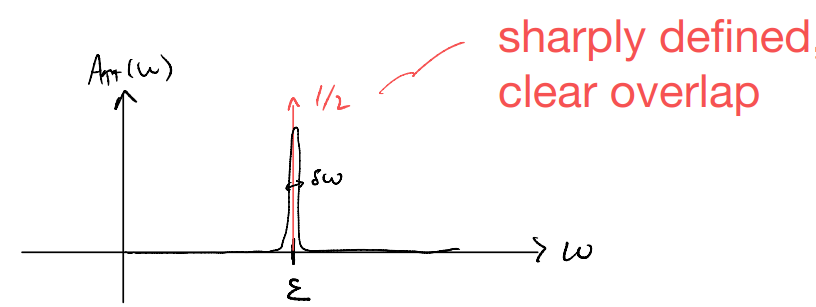
\includegraphics[width=\textwidth]{jupyterbook/data/fig/lec05-fig04.png}
\end{figure}

If this was an experimental result, how would we interpret it? There is a sharp ``resonance'' when we try to add an up electron with energy $\varepsilon$ to the ground state. The overlap is $\frac{1}{2}$. Suppose we can do similar experiments and measure $A_{\downarrow\downarrow}(\omega)$, as well as those associated with electron electron removal

\begin{figure}[ht]
    \centering
    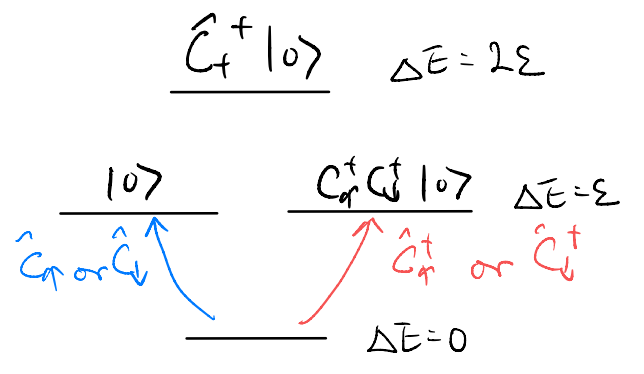
\includegraphics[width=\textwidth]{jupyterbook/data/fig/lec05-fig05.png}
\end{figure}

we will conclude:
\begin{enumerate}
    \item Adding $\hat{c}_{\uparrow}^{\dagger}$: sharp resonance with weight $\frac{1}{2}$
    \item Adding $\hat{c}_{\downarrow}^{\dagger}$: sharp resonance with weight $\frac{1}{2}$
    \item Removing $\hat{c}_{\uparrow}$: sharp resonance with weight $\frac{1}{2}$
    \item Removing $\hat{c}_{\downarrow}$: sharp resonance with weight $\frac{1}{2}$
\end{enumerate}

Further, IF we know the relevant Hilbert space is one orbital with spin-$\frac{1}{2}$ electrons, we can conclude
\begin{enumerate}[label=(\alph*)]
    \item We can both add and remove electron from the ground state, it must have $1$ electron
    \item The one electron is in some half-half state between spins up and down (equal weights above)
\end{enumerate}
\[ |\Omega \rangle =\frac{1}{\sqrt{2}}\left( \hat{c}_{\uparrow}^{\dagger}+e^{i\phi}\hat{c}_{\downarrow}^{\dagger} \right) |0\rangle \]
i.e., we know the ground state up to an undetermined phase!

Notes:
\begin{enumerate}
    \item We assumed above that we can choose to tunnel spin up versus down electrons independently. This is a kind of ``resolution'', giving ``spin-resolved'' spectral function (e.g., spin-polarized STM tips). If we don't have such spin resolution, we can only conclude (a) but not (b). More resolved means more knowledge
    \item For such a ``small'' system, one can imagine cooking up fancier measurements to ``better resolve'' the system. That's in the spirit of quantum tomography. We don't usually have the luxury of such measurement capability in many-body quantum systems so we won't go further down there.
\end{enumerate}

Let us next imagine plotting the spectral function for a general interacting many-body Hamiltonian
\[ A_{\alpha \alpha}\left( \omega \right) =\sum_n{\left| \langle n|\hat{c}_{\alpha}^{\dagger}|\Omega \rangle \right|^2\delta \left( \omega -\Delta E_n \right)}\]

\begin{figure}[ht]
    \centering
    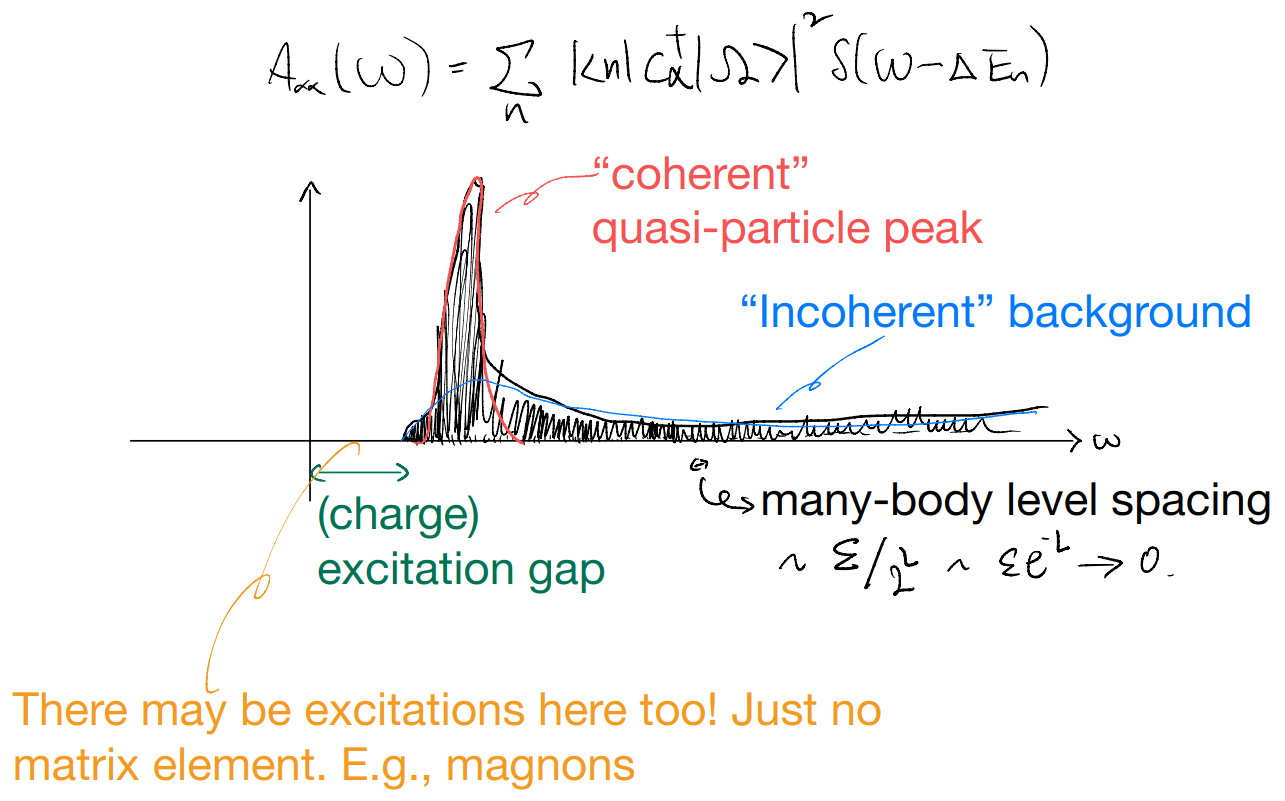
\includegraphics[width=\textwidth]{jupyterbook/data/fig/lec05-fig06.png}
\end{figure}

\begin{figure}[ht]
    \centering
    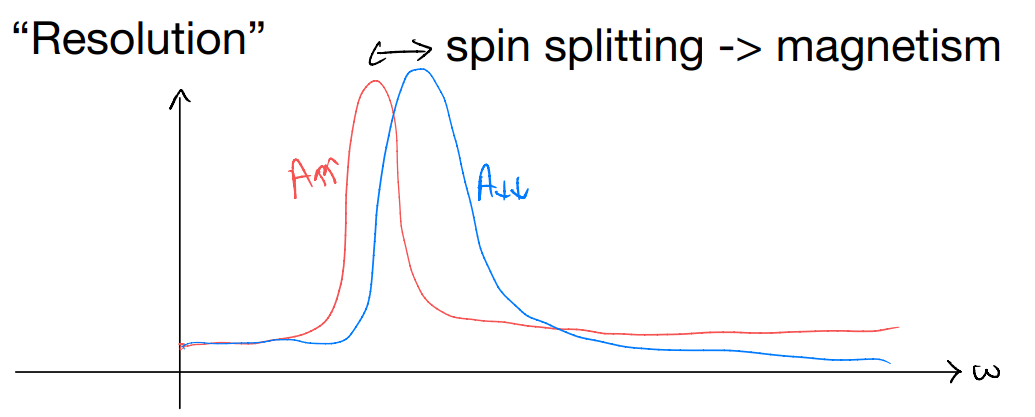
\includegraphics[width=\textwidth]{jupyterbook/data/fig/lec05-fig07.png}
\end{figure}

\begin{figure}[ht]
    \centering
    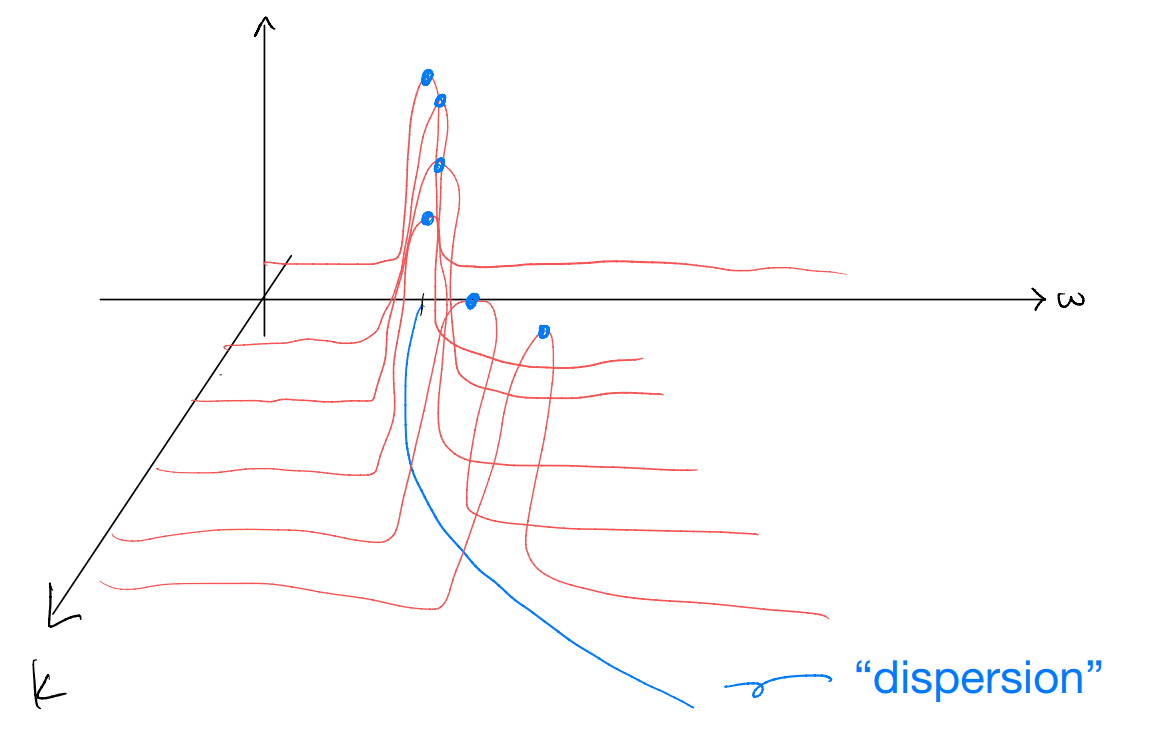
\includegraphics[width=\textwidth]{jupyterbook/data/fig/lec05-fig08.png}
\end{figure}

\begin{figure}[ht]
    \centering
    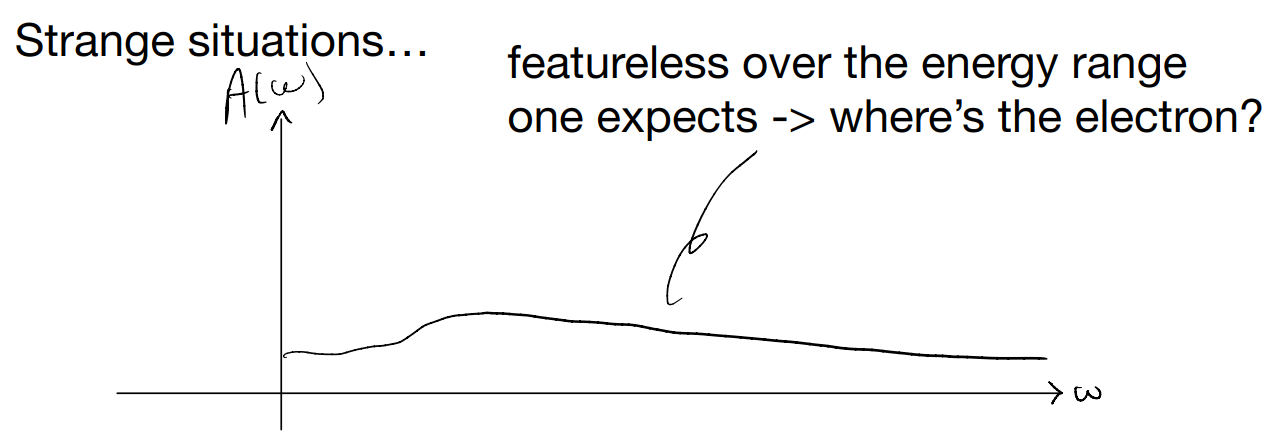
\includegraphics[width=\textwidth]{jupyterbook/data/fig/lec05-fig09.png}
\end{figure}

Strange situations: featureless over the energy range. If such a spectrum is observed, it suggests either
\begin{enumerate}
    \item the excitations cannot be understood as quasi-particles
    \item quasi-particles exist, but they have poor overlap with the physical electrons
\end{enumerate}

Either will be very interesting! But beyond our scope...

\section{A peek of the iceberg}

In the above, we chose in an ad hoc manner to consider the real-time Green's function
\[ G_{\alpha \alpha}\left( t \right) =\left( -i \right) \langle \Omega |\hat{c}_{\alpha}\left( t \right) \hat{c}_{\alpha}^{\dagger}\left( 0 \right) |\Omega \rangle \]
Since our ground state will have a some finite density of electrons to start with, it will be equally natural to consider, e.g.,
\[ G_{\alpha \alpha}^{\prime}\left( t \right) =\left( -i \right) \langle \Omega |\hat{c}_{\alpha}^{\dagger}\left( t \right) \hat{c}_{\alpha}\left( 0 \right) |\Omega \rangle \]
which contains information about electron removal from $|\Omega\rangle$.

In addition, we don't necessarily have to commit to the ``diagonal'' form with matched indices. E.g., if $\alpha$ denotes spatial indices, it would be natural to consider
\[ G_{xy}\left( t,t' \right) =\left( -i \right) \langle \Omega |\hat{c}_x\left( t \right) \hat{c}_{y}^{\dagger}\left( t' \right) |\Omega \rangle \]
Our commitment above on $t>0$ is also a bit ad hoc anyway. We should be free ask what happens if we compute ``negative time'' correlation function, at least as a theoretical gadget. Also, why not do something more than single electron addition (removal)? E.g.,
\[ G_{\alpha \alpha \gamma \delta}^{\prime\prime}\left( t_1,t_2,t_3,t_4 \right) =\left( -i \right) \langle \Omega |\hat{c}_{\alpha}\left( t_1 \right) \hat{c}_{\beta}\left( t_2 \right) \hat{c}_{\gamma}^{\dagger}\left( t_3 \right) \hat{c}_{\delta}^{\dagger}\left( t_4 \right) |\Omega \rangle \]
These discussions suggest that there is a huge zoo of possible ``Green's functionS'' to consider, and we need a way to organize them, e.g., fix some ordering on the time of ``insertions'', etc.

Such generalized Green's functions appear under different considerations, and we may want to give them different names, Nevertheless, they are all variations on the same tune, much like Schubert's trout quintet! More later...

\section{Impurity phonon coupling}

So far, we have discussed
\begin{enumerate}
    \item QHO: coherent states, displacement operator,...
    \item Free phonons: collection of decoupled QHOs
    \item Localized electrons: a primer into ``spectroscopy''
\end{enumerate}
Let us now integrate all these into one single problem: how could we use electrons to probe phonons?

\begin{figure}[ht]
    \centering
    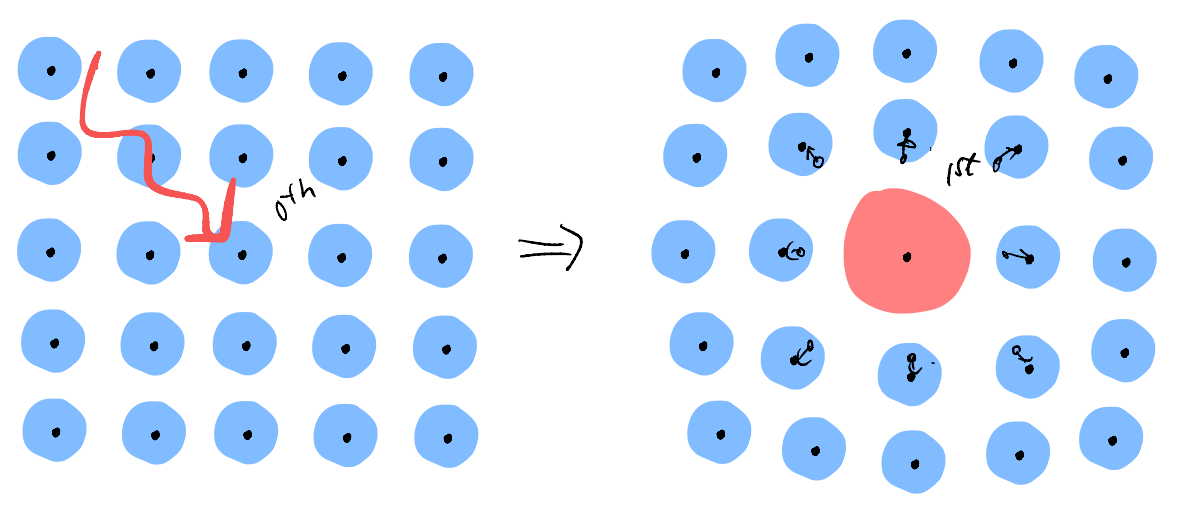
\includegraphics[width=\textwidth]{jupyterbook/data/fig/lec05-fig10.png}
\end{figure}

Similar to before, let us consider a single-site electronic problem:
\[ \hat{H}_e=\sum_{i=1}^N{\varepsilon _i\hat{c}_{i}^{\dagger}\hat{c}_i}\]
let us interpret the index $i$ as labeling some relevant orbitals $s,p,d,\cdots$ and for concreteness we suppose there are $N$ relevant orbitals in our problem. We also consider the free phonon Hamiltonian
\[ \hat{H}_{ph}=\sum_q{\omega _q\hat{a}_{q}^{\dagger}\hat{a}_q}\]
where we have dropped the zero-point energy for simplicity, and take a single branch with uniform masses.

Let us suppose the electronic Hamiltonian describes the electronic states of an impurity located at the origin. The size and shape of the electron cloud surrounding our impurity depends in general on the orbital index $i$. This, in turn, affect the equilibrium position of the neighboring atoms, e.g., a ``fatter'' electron cloud will push the neighboring atoms further away. We claim this coupling can be modelled as
\[ \hat{H}_{e-ph}=\sum_{i,q}{\hat{c}_{i}^{\dagger}\hat{c}_iM_{iq}\left( \hat{a}_q+\hat{a}_{q}^{\dagger} \right)}\]
We will see why in the next class.


\chapter{lec06 20220223}

Topics

\begin{enumerate}
    \item impurity-phonon coupling
    \item zero-temperature solution
    \item impurity spectral function
\end{enumerate}

Goals

\begin{enumerate}
    \item Applying the techniques to a less trivial and physically relevant problem
    \item Appreciating how we could probe phonons with electrons
\end{enumerate}

Last time, we began introducing an impurity-phonon problem:
\[ \hat{H}=\underset{\hat{H}_e}{\underbrace{\sum_{i=1}^N{\varepsilon _i\hat{c}_{i}^{\dagger}\hat{c}_i}}}+\underset{\hat{H}_{ph}}{\underbrace{\sum_q{\omega _q\hat{a}_{q}^{\dagger}\hat{a}_q}}}+\underset{\hat{H}_{e-ph}}{\underbrace{\sum_{i,q}{\hat{c}_{i}^{\dagger}\hat{c}_iM_{iq}\left( \hat{a}_q+\hat{a}_{q}^{\dagger} \right)}}}\]
It describes a system of an electronic impurity, whose state (occupancy of the orbitals indexed by $i$) affects the phonon through the last electron-phonon interaction term $\hat{H}_{e-ph}$. We will first sketch why $\hat{H}_{e-ph}$ takes the stated form.

Recall that our phonon Hamiltonian resulted from an expansion of the elastic potential energy about the equilibrium
\[ \hat{H}_{ph}=\sum_{r\alpha}{\frac{\hat{p}_{r}^{\alpha 2}}{2m}}+\frac{1}{2}\sum_{r,r'}{\left. \frac{\partial ^2\mathcal{V}}{\partial R_r\partial R_{r'}} \right|_0\left( \hat{R}_r-R_{r,0} \right) \left( \hat{R}_{r'}-R_{r',0} \right)}\]
\[ \hat{u}_r=\hat{R}_r-R_{r,0}\]
where $\hat{R}_r$ is the actual position, $R_{r,0}$ is the equilibrium position and $\hat{u}_r$ is the deviation from the equilibrium. As discussed, the equilibrium positions are now dependent on the electronic state
\[ R_{r,0}\rightarrow R_{r,0}+\delta R_{r,0}^{i}\]
where we expect $\delta R_{r,0}\approx 0$ for $r$ far from the impurity. To leading order, this leads to an $i$-dependent change of the phonon Hamiltonian
\begin{align*}
    \delta \hat{H}_{ph}^{i}&\sim -\sum_{r,r'}{\left. \frac{\partial ^2\mathcal{V}}{\partial R_r\partial R_{r'}} \right|_0\hat{u}_r\left( \delta R_{r'}^{i} \right)}+\delta E^i\\
    &=\sum_r{\left( M^i \right) _r\hat{u}_r}+\delta E^i
\end{align*}
where the first term is linear in $\hat{u}_r$ and $\delta E^i$ absorbs the electronic energies $\varepsilon_i$ (\emph{TODO strange expression}). We should now recast the operators into the phonon creation and annihilation $\hat{a}_q^\dagger$ and $\hat{a}_q$.
\[ \begin{cases}
	\hat{a}_q=\frac{1}{\sqrt{2}}\left( \sqrt{m\omega _q}\hat{u}_q+\frac{i}{\sqrt{m\omega _q}}\hat{p}_q \right)\\
	(\hat{a}_{-q})^{\dagger}=\frac{1}{\sqrt{2}}\left( \sqrt{m\omega _q}\hat{u}_q-\frac{i}{\sqrt{m\omega _q}}\hat{p}_q \right)\\
\end{cases}\]
\[ \Rightarrow \hat{u}_q=\frac{\hat{a}_q+\hat{a}_{q}^{\dagger}}{\sqrt{2m\omega _q}} \]
where we used
\[ \hat{u}_{-q}^{\dagger}=\hat{u}_q\]
\[ \hat{p}_{-q}^{\dagger}=\hat{p}_q\]
as one can see from the Fourier transform
\[ \hat{u}_q=\frac{1}{\sqrt{V}}\sum_r{e^{iq\cdot r}\hat{u}_r}\]
\[ \hat{u}_r=\frac{1}{\sqrt{V}}\sum_q{e^{-iq\cdot r}\hat{u}_q}\]
This gives the electron-dependent correction
\begin{align*}
    \delta \hat{H}_{ph}^{i}&=\sum_r{M_{r}^{i}\hat{u}_r}\\
    &=\sum_r{M_{r}^{i}\frac{1}{\sqrt{V}}\sum_q{e^{-iq\cdot r}\frac{\hat{a}_q+\hat{a}_{-q}^{\dagger}}{\sqrt{2m\omega _q}}}}\\
    &=\sum_q{\underbrace{\frac{1}{\sqrt{2m\omega _q}}\left( \frac{1}{\sqrt{V}}\sum_r{M_{r}^{i}e^{-iq\cdot r}} \right) }\left( \hat{a}_q+\hat{a}_{-q}^{\dagger} \right)}\\
    &=\sum_q{M_{q}^{i}\left( \hat{a}_q+\hat{a}_{-q}^{\dagger} \right)}\\
    &=\sum_q{\left( M_{q}^{i}\hat{a}_q+M_{-q}^{i}\hat{a}_{q}^{\dagger} \right)}
\end{align*}
let us further assert that $M_{r}^{i}=M_{-r}^{i}$ such that $M_{q}^{i}=M_{-q}^{i}$
\[ \Rightarrow \delta \hat{H}_{ph}^{i}=\sum_q{M_{q}^{i}\left( \hat{a}_q+\hat{a}_{q}^{\dagger} \right)}\]
Altogether, we have the impurity-phonon Hamiltonian (c.f. Mahan Chapter-4)
\[ \hat{H}=\underset{\hat{H}_e}{\underbrace{\sum_{i=1}^N{\varepsilon _i\hat{c}_{i}^{\dagger}\hat{c}_i}}}+\underset{\hat{H}_{ph}}{\underbrace{\sum_q{\omega _q\hat{a}_{q}^{\dagger}\hat{a}_q}}}+\underset{\hat{H}_{e-ph}}{\underbrace{\sum_{i,q}{\hat{c}_{i}^{\dagger}\hat{c}_iM_{iq}\left( \hat{a}_q+\hat{a}_{q}^{\dagger} \right)}}}\]
Note: is this a good approximation? Not necessarily. One should recognize what we have done above is quite schematic, and there are many possible reasons to object to our treatment, e.g.,
\begin{enumerate}
    \item The shift in equilibrium position is probably not as simple as what we have assumed. E.g., the shift may not be simply the sum of the individual orbital contribution
    \item There is no particular reason why terms like $\hat{c}_{i}^{\dagger}\hat{c}_j\left( \hat{a}_q+\hat{a}_{q}^{\dagger} \right) +h.c.$ are absent
\end{enumerate}

There are valid concerns. It's important to realize that, here, we are simply trying to motivate a toy model which is not crazy (doesn't mean it is directly applicable to any real problem). In particle, we will not dwell into details like the form of the coefficients $M_q^i$ etc. Those are important for really modelling an actual system. But our goal is simply to show how such problems could be approached, and from this illustrates relevant aspects of the one-particle Greens' function and spectral function.

\section{Exact solution}

We have discussed how the problems of free phonons and localized electrons are both exactly soluble. In our current problem, we have introduced a coupling between the two. Generally speaking, we cannot find exact solutions for such coupled problem. But we will now see that our toy model is really designed to remain exactly soluble.

To this end, let us introduce $\hat{n}_i=\hat{c}_{i}^{\dagger}\hat{c}_i$ being the electron number for the $i$-th orbital. It satisfies
\[ \hat{n}_{i}^{2}=\hat{c}_{i}^{\dagger}\hat{c}_i\hat{c}_{i}^{\dagger}\hat{c}_i=\hat{c}_{i}^{\dagger}\left( 1-\hat{c}_{i}^{\dagger}\hat{c}_i \right) \hat{c}_i=\hat{c}_{i}^{\dagger}\hat{c}_i=\hat{n}_i\]
\[ \Rightarrow \mathrm{eig}\left( \hat{n}_i \right) =0\quad \mathrm{or}\quad 1\]
Also, notice that $\left[ \hat{n}_i,\hat{n}_j \right] =0$. We can write the Hamiltonian as
\[ \hat{H}=\sum_{i=1}^N{\varepsilon _i\hat{n}_i}+\sum_q{\omega _q\hat{a}_{q}^{\dagger}\hat{a}_q}+\sum_{i,q}{\hat{n}_iM_{iq}\left( \hat{a}_q+\hat{a}_{q}^{\dagger} \right)}\]
We see readily that
\[ \left[ \hat{H},\hat{n}_i \right] =0,\quad \forall i=1,\cdots ,N\]
As such, the electron numbers are good quantum numbers, and we can decompose the full Hilbert space into the $2^N$ sectors labeled by
\[ \left( n_1,n_2,\cdots ,n_N \right) =\left( 0,0,\cdots ,0 \right) ,\left( 1,0,\cdots ,0 \right) ,\cdots ,\left( 1,1,\cdots ,1 \right) \]

For simplicity, let us denote one such ``configuration'' by $\{n_i\}$. The Hamiltonian restricted to one such sector becomes
\begin{align*}
    \left. \hat{H} \right|_{\left\{ n_i \right\}}&=\sum_{i=1}^N{\varepsilon _in_i}+\sum_q{\omega _q\hat{a}_{q}^{\dagger}\hat{a}_q}+\sum_q{\left( \sum_i{n_iM_{iq}} \right) \left( \hat{a}_q+\hat{a}_{q}^{\dagger} \right)}\\
    &=\sum_{i=1}^N{\varepsilon _in_i}+\sum_q{\omega _q\left( \hat{a}_{q}^{\dagger}+\frac{1}{\omega _q}\sum_i{n_iM_{iq}} \right) \left( \hat{a}_q+\frac{1}{\omega _q}\sum_i{n_iM_{iq}} \right)}\\
    &\qquad-\sum_q{\frac{1}{\omega _{q}}\left( \sum_i{n_iM_{iq}} \right) ^2}
\end{align*}
where we have used the usual trick of ``completing square''($(a+b)^2=a^2+b^2+2ab$)

In this restricted Hilbert space, the Hamiltonian acts only on the phonons. In addition, it contains only up to quadratic terms for the phonons, and so it remains exactly solvable. To construct the eigenstates, let us recall the displacement operator.
\[ \hat{D}_q\left( \alpha \right) =e^{\alpha \hat{a}_{q}^{\dagger}-\alpha ^*\hat{a}_q}\]
\[ \Rightarrow \hat{D}_q\left( \alpha \right) \hat{a}_q\hat{D}_{q}^{\dagger}\left( \alpha \right) =\hat{a}_q-\alpha \]
\[ \Rightarrow \hat{D}_q\left( \alpha \right) \hat{a}_{q}^{\dagger}\hat{D}_{q}^{\dagger}\left( \alpha \right) =\hat{a}_{q}^{\dagger}-\alpha ^*\]
Recall that $M_{iq}$ is real (TODO why), this gives
\begin{align*}
    &\left[ \prod_q{\hat{D}_q\left( \frac{1}{\omega _q}\sum_i{n_iM_{iq}} \right)} \right] \left( \left. \hat{H} \right|_{\left\{ n_i \right\}} \right) \left[ \prod_q{\hat{D}_{q}^{\dagger}\left( \frac{1}{\omega _q}\sum_i{n_iM_{iq}} \right)} \right] \\
    =&\sum_q{\omega _q\hat{a}_{q}^{\dagger}\hat{a}_q}+\sum_{i=1}^N{\varepsilon _in_i}-\sum_q{\frac{1}{\omega _{q}}\left( \sum_i{n_iM_{iq}} \right) ^2}
\end{align*}
where the first term is equivalent to the original phonon Hamiltonian, and other terms are just a number. We may define the energy
\[ \Delta \left( \left\{ n_i \right\} \right) =\sum_{i=1}^N{\varepsilon _in_i}-\sum_q{\frac{1}{\omega _q}\left( \sum_i{n_iM_{iq}} \right) ^2}\]
where the first term is the non-interacting orbital energy and the second term is the effective density-density interaction mediated by the phonons!

Note: this expression is slightly different from Mahan's who (somehow) assumed there is exactly one electron on the impurity, and so wrote $n_in_j=n_i\delta_{ij}$.

As such, we now know all the eigenstates and energy of our Hamiltonian. They can be labeled by two sets of integers
\begin{enumerate}
    \item $\{n_i\}$: occupation of the $i=1,\cdots,N$ electronic orbitals
    \item $\{m_q\}$: number of quanta in each of $q=1,\cdots,V$ phonon modes
\end{enumerate}
The energy is
\[ |\left\{ n_i \right\} ,\left\{ m_q \right\} \rangle :\quad \Delta \left( \left\{ n_i \right\} \right) +\sum_q{\omega _qm_q}\]
It may be instructive to sketch an energy level diagram corresponding to our solution. To illustrate the ideas, suppose we have three electronic orbitals in our problem, and they have ``bare'' orbital energy of $-\varepsilon _1=\varepsilon _2=\varepsilon _3=\varepsilon >0$

\begin{figure}[ht]
    \centering
    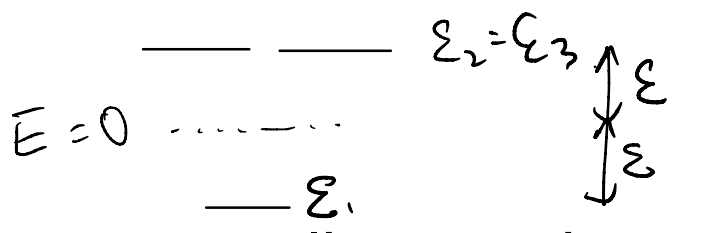
\includegraphics[width=\textwidth]{jupyterbook/data/fig/lec06-fig00.png}
\end{figure}

Without electron-phonon coupling, we have the eigen-energies

\begin{figure}[ht]
    \centering
    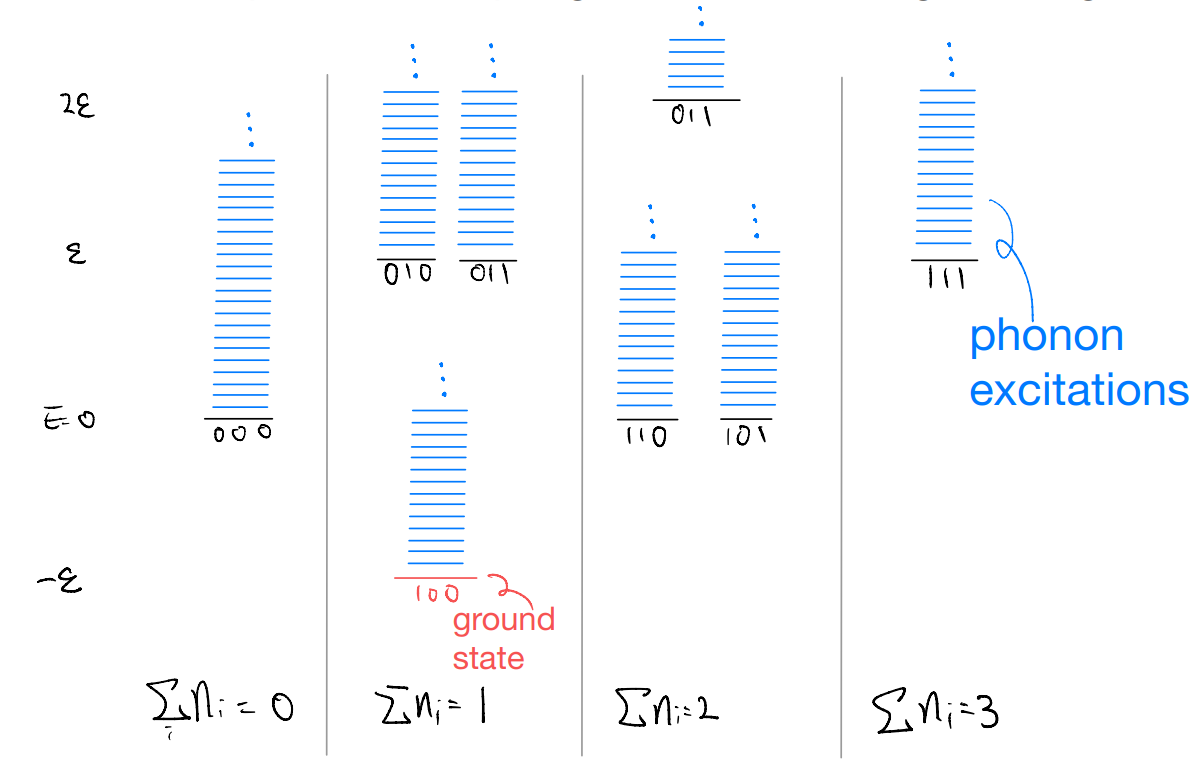
\includegraphics[width=\textwidth]{jupyterbook/data/fig/lec06-fig01.png}
\end{figure}

\noindent where for simplicity we considered an ``Einstein phonon'' model in which $\omega_q=\omega_E$ is $q$-independent. Otherwise, the phonon excitation should become a continuum as each mode (labeled by $q$) can have a different excitation energy.

Now, consider the effect of $\hat{H}_{e-ph}$, which we may treat as a perturbation to the level diagram above. A key simplifying assumption in our model (which enabled exact solutions) is that $[\hat{H},\hat{n}_i]=0$. In other words, even with the $e-ph$ coupling, we can think about each of the ``sub-block'' above individually.

\begin{figure}[ht]
    \centering
    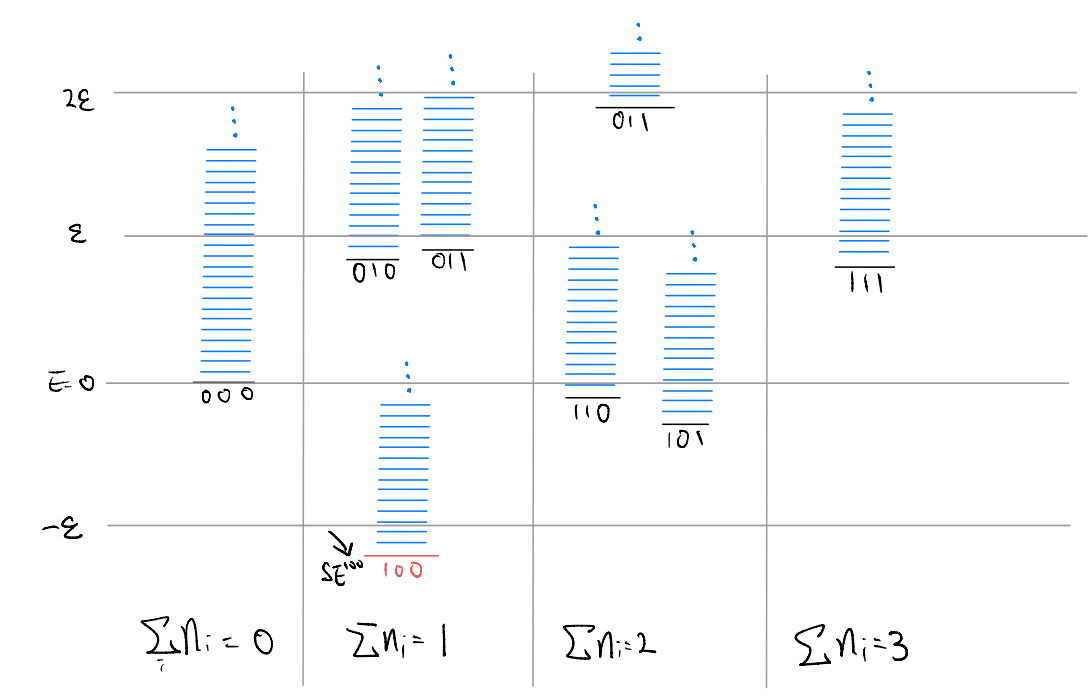
\includegraphics[width=\textwidth]{jupyterbook/data/fig/lec06-fig03.png}
\end{figure}

But this looks deceivingly simple! The phonon state $|\{m_q\} \rangle$ actually depends on the electronic occupation in a concealed manner. To see this more explicitly, let us write the Hamiltonian as
\begin{align*}
    \hat{H}=&\bigoplus_{\left\{ n_i \right\}}{\left. \hat{H} \right|_{\left\{ n_i \right\}}}\\
    =&\bigoplus_{\left\{ n_i \right\}}{\left( \sum_q{\hat{D}_{q}^{\dagger}\left( \frac{1}{\omega _q}\sum_i{n_iM_{iq}} \right) \omega _q\hat{a}_{q}^{\dagger}\hat{a}_q\hat{D}_q\left( \frac{1}{\omega _q}\sum_i{n_iM_{iq}} \right)}+\Delta \left( \left\{ n_i \right\} \right) \right)}
\end{align*}
where $\oplus$ is the direct sum over the $2^N$ independent sectors. It's still the ``same'' phonon Hamiltonian, but in different basis!

E.g., let $|\{m_q\}\rangle$ be the ``bare'' phonon eigenstates with phonon occupancy
\[ \hat{a}_{q}^{\dagger}\hat{a}_q\rightarrow m_q\]
Then the eigenstates of the Hamiltonian can be written as
\[ |\left\{ n_i \right\} ,\left\{ m_q \right\} \rangle =|\left\{ n_i \right\} \rangle \otimes \left[ \prod_q{\hat{D}_{q}^{\dagger}\left( \frac{1}{\omega _q}\sum_i{n_iM_{iq}} \right) |\left\{ m_q \right\} \rangle _0} \right] \]
Does this ``$i$-dependent basis rotation'' of the phonon matter? After all, the phonon energies are independent on the electronic configuration! The short answer is yes. To see why, we look into the electron's one-particle Green's function.

\section{Electron (impurity) Greens' function}

Let's look at a real-time one-particle Greens' function of the form
\[ G_{ii}\left( t \right) =-i\langle \Omega |\hat{c}_{i}^{\dagger}\left( t \right) \hat{c}_i\left( 0 \right) |\Omega \rangle \]
where $|\Omega \rangle$ is the ground state. We will compute $G_{ii}(t)$ in two ways
\begin{enumerate}
    \item Using the energy eigenstates we have derived. This is perhaps more transparent, but at the same time somewhat ``brute force'' and the solution approach looks a bit \emph{ad hoc}, since we cannot expect to solve the many-body Hamiltonian in general
    \item Solving the Heisenberg picture time evolution of the operator. This is probably the more systematic approach, and we will see that it allows for greater flexibility on the ground state
\end{enumerate}

Let us start with the ``brute force'' approach. For concreteness, we suppose the level scheme is the one drawn before, and so the ground state is
\[ |\Omega \rangle =|\left\{ 1,0,0 \right\} \rangle \otimes \prod_q{\hat{D}_{q}^{\dagger}\left( \frac{M_{1q}}{\omega _q} \right) |\left\{ 0_q \right\} \rangle _0}\]
\[ \hat{H}|\Omega \rangle =\Delta _{100}|\Omega \rangle \]
\[ \Delta _{100}=\varepsilon _1-\sum_q{\frac{M_{1q}^{2}}{\omega _q}}\]


\chapter{lec07 20220225}

Topics

\begin{enumerate}
    \item Impurity spectral function: Einstein model and numerical experiment
\end{enumerate}

Goals

\begin{enumerate}
    \item First example of a physically interesting spectral function
    \item Appreciating how to ``extract'' physical info from spectral function
\end{enumerate}

Consider the state with one electron removed:
\[ \hat{c}_1|\Omega \rangle =|\left\{ 0,0,0 \right\} \rangle \otimes \prod_q{\hat{D}_{q}^{\dagger}\left( \frac{M_{1q}}{\omega _q} \right) |\left\{ 0_q \right\} \rangle _0}\]
This is \emph{not} an eigenstate of $\hat{H}$! The eigenstates should have been
\[ |\left\{ 0,0,0 \right\} \rangle \otimes |\left\{ m_q \right\} \rangle \]
Non-eigenstates means states with dynamics. So now we consider
\begin{align*}
    G_{11}\left( t \right) &=\left( -i \right) \langle \Omega |\hat{c}_{1}^{\dagger}\left( t \right) \hat{c}_1\left( 0 \right) |\Omega \rangle \\
    &=\left( -i \right) \langle \Omega |e^{i\hat{H}t}\hat{c}_{1}^{\dagger}e^{-i\hat{H}t}\hat{c}_1|\Omega \rangle \\
    &=\left( -i \right) e^{i\Delta _{100}t}\langle \Omega |\hat{c}_{1}^{\dagger}e^{-i\hat{H}t}\hat{c}_1|\Omega \rangle \\
    &=\left( -i \right) e^{i\Delta _{100}t}\left[ \langle 0_q|_0\prod_q{\hat{D}_q\left( \frac{M_{1q}}{\omega _q} \right)} \right] \otimes \langle \left\{ 100 \right\} |\hat{c}_{1}^{\dagger}e^{-i\hat{H}t}\hat{c}_1\\
    &\qquad|\left\{ 100 \right\} \rangle \otimes \prod_q{\hat{D}_{q}^{\dagger}\left( \frac{M_{1q}}{\omega _q} \right)}|\left\{ 0_q \right\} \rangle _0\\
    &=\left( -i \right) e^{i\Delta _{100}t}\left[ \langle 0_q|_0\prod_q{\hat{D}_q\left( \frac{M_{1q}}{\omega _q} \right)} \right] \exp \left\{ -i\left. \hat{H} \right|_{\left\{ 000 \right\}}t \right\}\prod_q{\hat{D}_{q}^{\dagger}\left( \frac{M_{1q}}{\omega _q} \right)}|\left\{ 0_q \right\} \rangle _0\\
\end{align*}
But
\[ \left. \hat{H} \right|_{\left\{ 000 \right\}}==\sum_q{\omega _q\hat{a}_{q}^{\dagger}\hat{a}_q}+\Delta _{000}\]
\[ \Delta _{000}=0\]
We have
\[ G_{11}\left( t \right) =\left( -i \right) e^{i\Delta _{100}t}\prod_q{\left( \langle -\frac{M_{1q}}{\omega _q}|e^{-i\omega _q\hat{a}_{q}^{\dagger}\hat{a}_qt}|\frac{M_{1q}}{\omega _q}\rangle _0 \right)}\]
where the state in the bra and ket is the coherent state. This is just the ``propagator'' in the coherent-state basis!
\begin{align*}
    G_{11}\left( t \right) &=\left( -i \right) e^{i\Delta _{100}t}\prod_q{\left( \langle -\frac{M_{1q}}{\omega _q}|\frac{M_{1q}}{\omega _q}e^{-i\omega _qt}\rangle _0 \right)}\\
    &=\left( -i \right) e^{i\Delta _{100}t}\prod_q{\exp \left( \frac{M_{1q}^{2}}{\omega _{q}^{2}}e^{-i\omega _qt} \right) \exp \left( -\frac{M_{1q}^{2}}{\omega _{q}^{2}} \right)}
\end{align*}
Let's define $g_q=\left( \frac{M_{1q}}{\omega _q} \right) ^2$, then
\[ G_{11}\left( t \right) =\left( -i \right) e^{i\Delta _{100}t}\exp \left( \sum_q{g_q\left( e^{-i\omega _qt}-1 \right)} \right) \]
To make further progress, consider again the Einstein model with
\[ \omega _q=\omega _E,\quad \forall q\]
Let $g=\sum_q{g_q}$, then
\[ G_{11}\left( t \right) =\left( -i \right) e^{i\Delta _{100}t}\exp \left( ge^{-i\omega _Et}-g \right) \]
We can now consider the Fourier transform
\begin{align*}
    G_{11}\left( \omega \right) &=\left( -i \right) e^{-g}\lim_{\eta \rightarrow 0^+} \int_0^{\infty}{dte^{i\Delta _{100}t}e^{i\omega t}e^{-\eta t}\exp \left( ge^{-i\omega _Et} \right)}\\
    &=\left( -i \right) e^{-g}\sum_{l=0}^{\infty}{\lim_{\eta \rightarrow 0^+} \int_0^{\infty}{dt\frac{g^l}{l!}e^{i\left( \omega +\Delta _{100}-l\omega _E+i\eta \right) t}}}\\
    &=e^{-g}\sum_{l=0}^{\infty}{\lim_{\eta \rightarrow 0^+} \frac{g^l}{l!}\frac{1}{\omega +\Delta _{100}-l\omega _E+i\eta}}\\
\end{align*}
and same as before we find the spectral function
\begin{align*}
    A_{11}\left( \omega \right) &=\frac{-1}{\pi}\mathrm{Im}G_{11}\left( \omega \right) \\
    &=\sum_{l=0}^{\infty}{e^{-g}\frac{g^l}{l!}\delta \left( \omega -\left( -\Delta _{100}+l\omega _E \right) \right)}
\end{align*}
\[ \Delta _{100}=\varepsilon _1-\sum_q{\frac{M_{1q}^{2}}{\omega _q}}=\varepsilon _1-\omega _Eg<0\]
The spectral function is the sum of delta functions. For which $l$ do we get the highest weight?
\[ \frac{g^{l+1}}{\left( l+1 \right) !}=\left( \frac{g}{l+1} \right) \left( \frac{g^l}{l!} \right) \]
increasing for $l<g-1$, decreasing for $l>g-1$

\begin{figure}[ht]
    \centering
    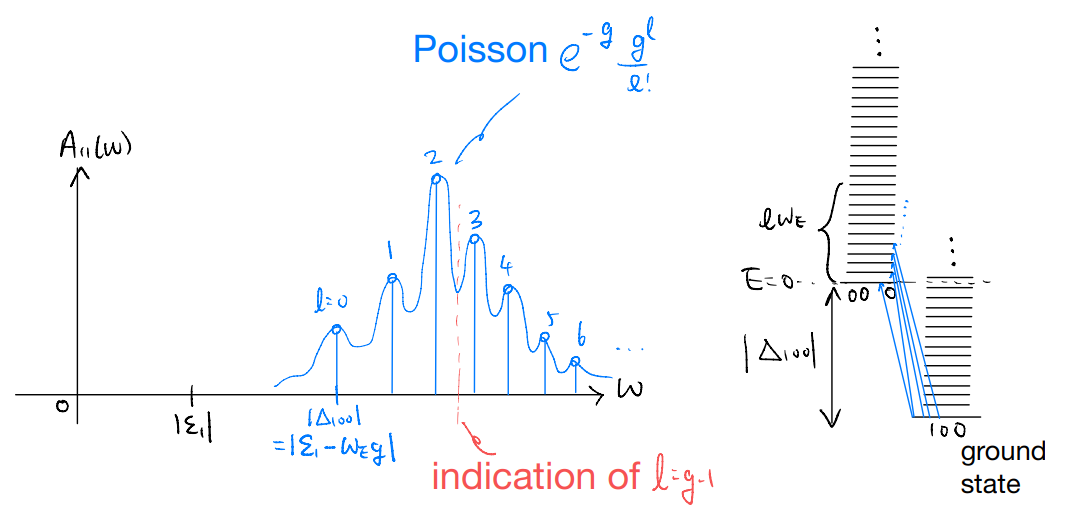
\includegraphics[width=\textwidth]{jupyterbook/data/fig/lec07-fig00.png}
\end{figure}

Interpretation: when we try to remove an electron, we discover that in the ground state the "electron" is actually dressed by the phonons. With strong coupling ($g\gg 1$), the dominant spectral peak is far from the bare electronic orbital contribution of $|\Delta_{100}|$.

Notes:
\begin{enumerate}
    \item The Einstein model is simple by design, and enables very explicit computation of the frequency-space Green's function (and hence spectral function). Our real-time solution, however, holds for more general phonon dispersion. When we deviate from the Einstein model we should start seeing deviation from the ``sum of delta function'' form of the spectral function
    \item More interestingly, one should ask what happens for acoustic phonons which have $\omega_q\to 0$ as $q\to 0$. Recall the strength of the $e-ph$ coupling was parameterized by $g_q=\left(\frac{M_{iq}}{\omega_q}\right)^2$. If $M_{iq}$ stays finite and $\omega_q\to 0$, we have diverging coupling and hence energies etc.!
\end{enumerate}

This is a rather general feature: low-energy modes are ``dangerous'' because they are easy to excite. In finding the ground state, one should, generally speaking, check how the ``fluctuations'' (lowest excitations) could destabilize the ground state. This amounts to a kind of self-consistency check. If the assumed ground state implies strong fluctuations which kills itself, the ground state does not actually ``form''. This is the key physical picture behind the Merlin-Wagner theorem on the absence of spontaneous continuous symmetry breaking in low dimensions.

Now, back to our impurity-phonon problem: physically, the acoustic phonons have vanishing frequency in the long-wavelength limit because they are Goldstone modes. The Goldstones exist because of symmetries, and are correspondingly constrained by symmetries. In our context, the catastrophe is avoided by having a ``derivative coupling'', such that the $e-ph$ coupling has a momentum dependence of $M_{iq}\propto q$ as $q\to 0$. This gives a finite coupling strength as both $M_{iq}$ and $\omega_q$ vanish linearly in $q$.

Note: play with the uploaded Python code if you want to explore what happens beyond the Einstein model.


\chapter{lec08 20220302}

Topics

\begin{enumerate}
    \item Impurity spectral function: solving again with Heisenberg
    \item Dyson series, time ordering, and time-ordered exponential
\end{enumerate}

Goals

\begin{enumerate}
    \item Learning how to deal with time-dependent perturbations
\end{enumerate}

\section{Solving again: Heisenberg picture}

Our solution for the impurity (one-electron) spectral function was satisfactory (I think), in the sense that we have found a concrete expression which does encode a lot of interesting physics (e.g., enable numerical simulation, and analytical solution with the simplified Einstein phonons). Yet, it is also clear that our calculation approach worked because we have an exactly solved model. This is a luxury to have, and oftentimes people take ``exactly solubility'' to equate to ``boring''. (Of course, this is subjected to personal taste)

The bottom line is, our problem was exactly solvable because it ultimately decouples into independent QHO (shifted phonon Hamiltonian) and fermions (individually conserved particle number). We only have a minimal degree of interactions in our model, namely, the phonon-mediated density-density interactions between the electrons.

Our course is called ``Quantum many-body theory'', and apparently I cannot avoid introducing techniques for solving more general interacting many-body problems! This motivates to go through a more complicated approach of solving the same problem again, through the Heisenberg picture.

Recall in the Heisenberg picture the states are stationary, and the operators evolve according to
\[ \hat{O}_H\left( t \right) =e^{i\hat{H}t}\hat{O}_Se^{-i\hat{H}t}\]
their time evolution is governed by the equation of motion
\[ i\partial _t\hat{O}_H\left( t \right) =\left[ \hat{O}_H\left( t \right) ,\hat{H} \right] _H\]
everything below will be in the Heisenberg picture, and we drop the subscript. Here we want to compute the real-time Green's function
\[G_{ii}\left( t \right) =\langle \Omega |\hat{c}_{i}^{\dagger}\left( t \right) \hat{c}_i\left( 0 \right) |\Omega \rangle \]
and so we would want to compute the time evolution of $\hat{c}_i^\dagger(t)$ under the Hamiltonian
\[ \hat{H}=\sum_{i=1}^N{\varepsilon _i\hat{n}_i}+\sum_q{\omega _q\hat{a}_{q}^{\dagger}\hat{a}_q}+\sum_{i,q}{\hat{n}_iM_{iq}\left( \hat{a}_q+\hat{a}_{q}^{\dagger} \right)}\]
So we first find the equation of motion for $\hat{c}_i(t)$. Notice
\begin{align*}
    \left[ \hat{c}_{i}^{\dagger}\left( t \right) ,\hat{n}_j\left( t \right) \right] &=\left[ \hat{c}_{i}^{\dagger}\left( t \right) ,\hat{c}_{j}^{\dagger}\left( t \right) \hat{c}_j\left( t \right) \right] \\
    &=\delta _{ij}\left( \hat{c}_{i}^{\dagger}\left( t \right) \left[ \hat{c}_{i}^{\dagger}\left( t \right) ,\hat{c}_i\left( t \right) \right] \right) \\
    &=\delta _{ij}\hat{c}_{i}^{\dagger}\left( t \right) \left( 2\hat{c}_{i}^{\dagger}\left( t \right) \hat{c}_i\left( t \right) -1 \right) \\
    &=-\delta _{ij}\hat{c}_{i}^{\dagger}\left( t \right)
\end{align*}
we then have
\begin{align*}
    i\partial _t\hat{c}_{i}^{\dagger}\left( t \right) &=\left[ \hat{c}_{i}^{\dagger}\left( t \right) ,\hat{H} \right] \\
    &=\sum_j{\left[ \hat{c}_{i}^{\dagger}\left( t \right) ,\varepsilon _j\hat{n}_j\left( t \right) +\hat{n}_j\left( t \right) \sum_q{M_{jq}\left( \hat{a}_q\left( t \right) +\hat{a}_{q}^{\dagger}\left( t \right) \right)} \right]}\\
    &=-\left( \varepsilon _i+\sum_q{M_{iq}\left( \hat{a}_q\left( t \right) +\hat{a}_{q}^{\dagger}\left( t \right) \right)} \right) \hat{c}_{i}^{\dagger}\left( t \right) \\
    &=\hat{O}\left( t \right) \hat{c}_{i}^{\dagger}\left( t \right)
\end{align*}
\[ \hat{O}\left( t \right) =-\varepsilon _i-\sum_q{M_{iq}\left( \hat{a}_q\left( t \right) +\hat{a}_{q}^{\dagger}\left( t \right) \right)}\]
compared to our earlier ``single-site'' electronic model (c.f. Lecture-4), the difference is that the orbital energy $\varepsilon_i$ is now promoted to a time-dependent operator. The ``operators'' act on the phonon Fock space, and reflects the electron-phonon coupling. The time-dependence comes from the time evolution of the phonon operators, which reflects their dynamics.

This, therefore, implies that we have to also solve for the time-evolution of the phonon operators, Again, we first notice
\[ \left[ \hat{a}_q\left( t \right) ,\hat{a}_{q'}^{\dagger}\left( t \right) \right] =\delta _{qq'}\]
\[ \Rightarrow \quad \left[ \hat{a}_q\left( t \right) ,\hat{a}_{q'}^{\dagger}\left( t \right) \hat{a}_{q'}\left( t \right) \right] =\delta _{qq'}\hat{a}_q\left( t \right) \]
and so the equation of motion is
\begin{align*}
    i\partial _t\hat{a}_q\left( t \right) &=\left[ \hat{a}_q\left( t \right) ,\sum_{q'}{\left( \omega _{q'}\hat{a}_{q'}^{\dagger}\hat{a}_{q'}+\sum_i{\hat{n}_iM_{iq'}\left( \hat{a}_{q'}+\hat{a}_{q'}^{\dagger} \right)} \right)} \right] \\
    &=\omega _q\hat{a}_q\left( t \right) +\sum_i{\hat{n}_iM_{iq}}
\end{align*}
the $e-ph$ coupling again leads to a new piece, which requires us to consider
\[ i\partial _t\hat{n}_i\left( t \right) =\left[ \hat{n}_i\left( t \right) ,\hat{H} \right] =0\]
which means $\hat{n}_i(t)$ is an ``integral of motion'' and stays constant $\hat{n}_i(t)=\hat{n}_i$.

Note: We have basically set up a hierarchy of equation of motions (EOM): when we try to solve for the evolution of an operator, we see that its EOM contains some other operators, and we have to proceed with finding the EOM of these other operators etc. Such hierarchy is not closed in general, which makes it impossible to write down a closed set of equations (and let alone finding the exact solution). From this lens, our model is exactly solved in that the hierarchy terminates, and we only need to consider the coupled equations for $\hat{c}_i^\dagger (t)$ and $\hat{a}_q(t)$. We may first solve
\[ i\partial _t\hat{a}_q\left( t \right) =\omega _q\hat{a}_q\left( t \right) +\sum_i{\hat{n}_iM_{iq}}\]
Let
\[ \hat{a}_q\left( t \right) =\hat{A}+\hat{B}e^{-i\omega_qt}\]
\[ i\partial _t\hat{a}_q\left( t \right) =\omega _q\hat{B}e^{-i\omega t}=\omega _q\left( \hat{a}_q\left( t \right) -\hat{A} \right) \]
comparing the equations above,
\[ -\omega _q\hat{A}=\sum_i{\hat{n}_iM_{iq}}\]
\[ \Rightarrow\quad \hat{a}_q\left( t \right) =-\sum_i{\hat{n}_i\frac{M_{iq}}{\omega _q}}+\hat{B}e^{-i\omega _qt}\]
\[ \hat{a}_q\left( 0 \right) =-\sum_i{\hat{n}_i\frac{M_{iq}}{\omega _q}}+\hat{B}\]
\[ \Rightarrow \quad \hat{B}=\hat{a}_q\left( 0 \right) +\sum_i{\hat{n}_i\frac{M_{iq}}{\omega _q}}\]
\[ \Rightarrow \quad \hat{a}_q\left( t \right) +\sum_i{\hat{n}_i\frac{M_{iq}}{\omega _q}}=\left( \hat{a}_q\left( 0 \right) +\sum_i{\hat{n}_i\frac{M_{iq}}{\omega _q}} \right) e^{-i\omega _qt}\]
Looks familiar? This simply reflects our earlier observation that, the ``eigen'' phonon operators in the $\{n_i\}$ sector is related to the bare one (i.e., in the absence of $e-ph$ coupling) by a shift using the displacement operator.

To simplify notation, let us define
\[ \hat{a}_{q}^{\left\{ n_i \right\}}\left( t \right) =\hat{a}_q\left( t \right) +\sum_i{\hat{n}_i\frac{M_{iq}}{\omega _q}}\]
Then we simply have
\[ \hat{a}_{q}^{\left\{ n_i \right\}}\left( t \right) =\hat{a}_{q}^{\left\{ n_i \right\}}\left( 0 \right) e^{-i\omega _qt}\]
With this preparation we can go back to study the time-evolution of  the fermion operator
\[ i\partial _t\hat{c}_{i}^{\dagger}\left( t \right) =\hat{O}\left( t \right) \hat{c}_{i}^{\dagger}\left( t \right) \]
\begin{align*}
    \hat{O}\left( t \right) &=-\varepsilon _i-\sum_q{M_{iq}\left( \hat{a}_q\left( t \right) +\hat{a}_{q}^{\dagger}\left( t \right) \right)}\\
    &=-\varepsilon _i-\sum_q{M_{iq}\left( \hat{a}_{q}^{\left\{ n_i \right\}}\left( t \right) +\hat{a}_{q}^{\left\{ n_i \right\} \dagger}\left( t \right) -2\sum_j{\hat{n}_j\frac{M_{jq}}{\omega _q}} \right)}
\end{align*}
How do we solve this? Recall, if we have a simple function
\[ i\partial _tf\left( t \right) =g\left( t \right) f\left( t \right) \]
\[ \Rightarrow \,\,f\left( t \right) =f\left( 0 \right) \exp \left( -i\int_0^t{g\left( t' \right) dt'} \right) \]
\begin{align*}
    i\partial _tf\left( t \right) &=f\left( 0 \right) \left( i\partial _t\exp \left( -i\int_0^t{g\left( t' \right) dt'} \right) \right) \\
    &=f\left( 0 \right) \left( \partial _t\int_0^t{g\left( t' \right) dt'} \right) \exp \left( -i\int_0^t{g\left( t' \right) dt'} \right) \\
    &=g\left( t \right) f\left( t \right)
\end{align*}
It is then tempting to declare our formal solution is simply
\[ \hat{c}_{i}^{\dagger}\left( t \right) \stackrel{?}{=}\exp \left( -i\int_0^t{\hat{O}\left( t' \right) dt'} \right) \hat{c}_{i}^{\dagger}\left( 0 \right) \]
But we should Remember the meaning of the exponential here is that it is a formal power series!
\begin{align*}
    \hat{c}_{i}^{\dagger}&\stackrel{?}{=}\sum_{n=0}^{\infty}{\frac{\left( -i \right) ^n}{n!}\left[ \int_0^t{dt'\hat{O}\left( t' \right)} \right] ^n}\hat{c}_{i}^{\dagger}\left( 0 \right)\\
    &=\left( 1-i\int_0^t{dt_1\hat{O}\left( t_1 \right)}+\frac{\left( -i \right) ^2}{2}\int_0^t{dt_1\int_0^t{dt_2\hat{O}\left( t_1 \right) \hat{O}\left( t_2 \right)}}+\cdots \right) \hat{c}_{i}^{\dagger}\left( 0 \right)
\end{align*}
\[i\partial _t\hat{c}_{i}^{\dagger}\left( t \right) \stackrel{?}{=}\left\{ \hat{O}\left( t \right) -\frac{i}{2}\left[ \hat{O}\left( t \right) \left( \int_0^t{dt_2\hat{O}\left( t_2 \right)} \right) +\left( \int_0^t{dt_1\hat{O}\left( t_1 \right)} \right) \hat{O}\left( t \right) \right] +\cdots \right\} \hat{c}_{i}^{\dagger}\left( 0 \right) \]
versus
\[ \hat{O}\left( t \right) \hat{c}_{i}^{\dagger}\left( t \right) =\hat{O}\left( t \right) \left( 1-i\int_0^t{dt_1\hat{O}\left( t_1 \right)}+\cdots \right) \hat{c}_{i}^{\dagger}\left( 0 \right) \]
the two expression agree to this order only if
\[ \frac{1}{2}\left[ \hat{O}\left( t \right) \left( \int_0^t{dt_2\hat{O}\left( t_2 \right)} \right) +\left( \int_0^t{dt_1\hat{O}\left( t_1 \right)} \right) \hat{O}\left( t \right) \right] =\hat{O}\left( t \right) \int_0^t{dt_1\hat{O}\left( t_1 \right)}\]
\[ \Rightarrow \quad \left[ \int_0^t{dt_1\hat{O}\left( t_1 \right)},\hat{O}\left( t \right) \right] =0\]
But the ``same'' operator at different times may not commute with ``itself''! E.g., consider a single QHO, let
\[ \hat{O}\left( t \right) =\hat{a}\left( t \right) +\hat{a}^{\dagger}\left( t \right) =\hat{a}\left( 0 \right) e^{-i\omega t}+\hat{a}^{\dagger}\left( 0 \right) e^{i\omega t}\]
\begin{align*}
    \left[ \hat{O}\left( t_1 \right) ,\hat{O}\left( t_2 \right) \right] &=\left[ \hat{a}\left( 0 \right) e^{-i\omega t_1}+\hat{a}^{\dagger}\left( 0 \right) e^{i\omega t_1},\hat{a}\left( 0 \right) e^{-i\omega t_2}+\hat{a}^{\dagger}\left( 0 \right) e^{i\omega t_2} \right] \\
    &=\left[ \hat{a}^{\dagger}\left( 0 \right) ,\hat{a}\left( 0 \right) \right] e^{i\omega \left( t_1-t_2 \right)}+\left[ \hat{a}\left( 0 \right) ,\hat{a}^{\dagger}\left( 0 \right) \right] e^{-i\omega \left( t_1-t_2 \right)}\\
    &=-2i\sin \omega \left( t_1-t_2 \right)
\end{align*}
In other words, the ``solution'' we proposed is problematic when such non-commutation arises. To solve the problem, we have two (equivalent) pictures:

(1) Discretize then limit

Consider a small time interval $\delta_t$. To leading order in $\delta_t$, we may pretend $\hat{O}(t)\approx \hat{O}(t+\delta_t)$ is constant. Then we have
\[ \hat{c}_{i}^{\dagger}\left( t+\delta _t \right) \approx e^{-i\hat{O}\delta _t}\hat{c}_{i}^{\dagger}\left( t \right) \]
Doing this successively, we can approximate a long-time evolution

\begin{figure}[ht]
    \centering
    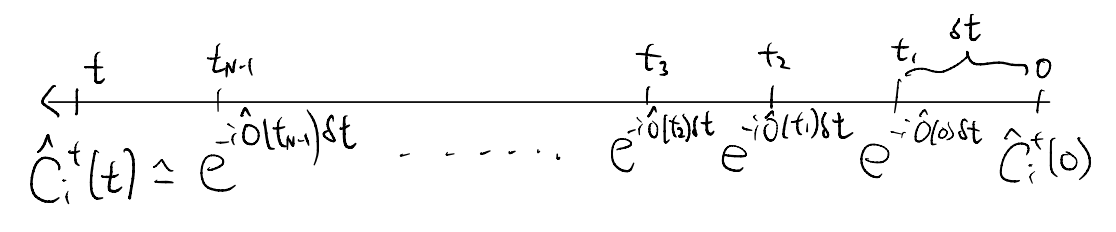
\includegraphics[width=\textwidth]{jupyterbook/data/fig/lec08-fig00.png}
\end{figure}

and we claim this becomes exact in the limit
\[ \hat{c}_{i}^{\dagger}\left( t \right) =\lim_{N\rightarrow \infty} e^{-i\hat{O}\left( t_{N-1} \right) t/N}\cdots e^{-i\hat{O}\left( t_n \right) t/N}\cdots e^{-i\hat{O}\left( t_1 \right) t/N}e^{-i\hat{O}\left( 0 \right) t/N}\hat{c}_{i}^{\dagger}\left( 0 \right) \]
\[ t_n=\frac{nt}{N}\]

Remarks:

\begin{enumerate}
    \item This is quite intuitive, but at the same time we did not justify its validity (e.g., error estimate, convergence of limit etc.). We will not worry about these problems, and just declare it's okay.
    \item How might one even try to evaluate this? In the case when the operators are more general (complicated), it may not be feasible to work out everything explicitly and exactly using only the abstract operator algebra.
\end{enumerate}

One natural way forward is to go back to some explicit ``basis'', e.g., in a coordinate-space basis we may replace $\hat{x}\to x$. Yet, in the same basis momentum $\hat{p}\to -i\partial_x$ is still an operator. Rather, it becomes a number only if we go to a momentum basis. Such dichotomy of ``what is easy'' is the defining feature (trouble) of quantum mechanics.

But we are considering small time intervals! Their failure to commute enters in $O(\delta_t^2)$. In other words, we can insert resolutions of identity for both $x$ and $p$ at each time-slice, and then treat them as commuting variables (since they are now only real numbers) in the limit $\delta_t\to 0$! This is the path integral picture.

(2) Fix the ordering up

Alternatively, we can also try to ``repair'' our good old solution
\[ \hat{c}_{i}^{\dagger}\left( t \right) \sim \exp \left( -i\int_0^t{dt'\hat{O}\left( t' \right)} \right) \hat{c}_{i}^{\dagger}\left( 0 \right) \]
after all, we know it is perfectly fine when $\hat{O}(t)$ at different times commute. (In particular, when it is time-independent.)

To this end, we first notice if we write
\[ \hat{c}_{i}^{\dagger}\left( t \right) =\hat{U}\left( t \right) \hat{c}_{i}^{\dagger}\left( 0 \right) \]
with the ``initial condition'' $\hat{U}\left( 0 \right) =1$, and demand it to be a solution to
\[ i\partial _t\hat{c}_{i}^{\dagger}\left( t \right) =\hat{O}\left( t \right) \hat{c}_{i}^{\dagger}\left( t \right) \]
\[ \Rightarrow \quad \left( i\partial _t\hat{U}\left( t \right) \right) \hat{c}_{i}^{\dagger}\left( 0 \right) =\hat{O}\left( t \right) \hat{U}\left( t \right) \hat{c}_{i}^{\dagger}\left( 0 \right) \]
\[ \Rightarrow \quad i\partial _t\hat{U}\left( t \right) =\hat{O}\left( t \right) \hat{U}\left( t \right) \]
We can as well go from the ``differential'' equation to an ``integral'' equation
\[ \hat{U}\left( t \right) =\hat{U}\left( 0 \right) -i\int_0^t{dt_1\hat{O}\left( t_1 \right) \hat{U}\left( t_1 \right)}\]
This isn't quite ``solving'' $\hat{U}(t)$ yet, as it still appears on both left- and right-hand sides. But we may now iterate
\begin{align*}
    \hat{U}\left( t \right) &=1-i\int_0^t{dt_1\hat{O}\left( t_1 \right) \hat{U}\left( t_1 \right)}\\
    &=1-i\int_0^t{dt_1\hat{O}\left( t_1 \right) \left[ 1-i\int_0^{t_1}{dt_2\hat{O}\left( t_2 \right) \hat{U}\left( t_2 \right)} \right]}\\
    &=1-i\int_0^t{dt_1\hat{O}\left( t_1 \right)}+\left( -i \right) ^2\int_0^t{dt_1\int_0^{t_1}{dt_2\hat{O}\left( t_1 \right) \hat{O}\left( t_2 \right) \hat{U}\left( t_2 \right)}}\\
    &=1-i\int_0^t{dt_1\hat{O}\left( t_1 \right)}+\left( -i \right) ^2\int_0^t{dt_1\int_0^{t_1}{dt_2\hat{O}\left( t_1 \right) \hat{O}\left( t_2 \right)}}\\
    &\qquad+\left( -i \right) ^3\int_0^t{dt_1\int_0^{t_1}{dt_2\int_0^{t_2}{dt_3\hat{O}\left( t_1 \right) \hat{O}\left( t_2 \right) \hat{O}\left( t_3 \right) \hat{U}\left( t_3 \right)}}}\\
    &\vdots
\end{align*}
we thus also get a formal power series solution to $\hat{U}(t)$, with the general form of the $n$-th term given by
\[ \hat{U}\left( t \right) =\sum_{n=0}^{\infty}{\left( -1 \right) ^n\int_0^t{dt_1\int_0^{t_1}{dt_2}\cdots \int_0^{t_{n-1}}{dt_n\hat{O}\left( t_1 \right) \hat{O}\left( t_2 \right) \cdots \hat{O}\left( t_n \right)}}}\]
This is called the ``Dyson series''. We see that it is quite ``close'' to the expansion of the exponential. But with two important differences:
\begin{enumerate}
    \item we are missing a factor of $n!$ in the factorial.
    \item the multiple time variables are ordered since each is bounded by the preceding one under the integral:
    \[ t_n<t_{n-1}<\cdots <t_2<t_1<t\]
    such ordering is the key to repairing our ``exponential solution'' with regards to the non-commuting nature $\left[ \hat{O}\left( t \right) ,\hat{O}\left( t' \right) \right] \ne 0$.
\end{enumerate}

Observation (1) invites us to ``over count'' the terms by treating the different $\hat{O}(t_n)$ more equally, and in doing so we have to replace
\[ \int_0^{t_{n-1}}{dt_n}\mapsto \int_0^t{dt_n}\]
At the same time, observation (2) instructs us to be disciplined when we perform such over-counting, since otherwise we screw up with the ordering of the operators demanded by the non-commuting nature of $\hat{O}(t)$ at different times. Combined, we claim
\begin{align*}
    \hat{U}\left( t \right) &=\sum_{n=0}^{\infty}{\frac{\left( -1 \right) ^n}{n!}\mathcal{T} \left[ \int_0^t{dt_1\int_0^t{dt_2}\cdots \int_0^t{dt_n\hat{O}\left( t_1 \right) \hat{O}\left( t_2 \right) \cdots \hat{O}\left( t_n \right)}} \right]}\\
    &=\mathcal{T} \left[ \exp \left\{ -i\int_0^t{dt'\hat{O}\left( t' \right)} \right\} \right]
\end{align*}
called the ``time-ordered exponential''. Here $\mathcal{T}$ is the ``time-ordering'' operator
\[ \mathcal{T} \left[ \hat{A}\hat{B}\hat{C}\hat{D} \right] =\hat{D}\hat{B}\hat{A}\hat{C}\]
for
\begin{figure}[ht]
    \centering
    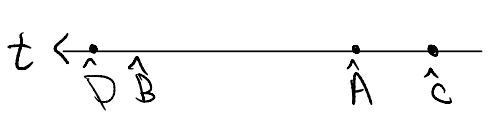
\includegraphics[width=\textwidth]{jupyterbook/data/fig/lec08-fig01.png}
\end{figure}


\chapter{lec09 20220302}

Topics

\begin{enumerate}
    \item Impurity spectral function from the Heisenberg picture: Dyson series and time-ordered exponential
    \item ``Sub-problem'' driven QHO
    \item introduction to Normal order and Wick's theorem
\end{enumerate}

Goals

\begin{enumerate}
    \item Getting familiar with time-ordering
    \item Starting to appreciate how to evaluate time-ordered exponential
    \item A primer to many-body perturbation theory
\end{enumerate}

Last lecture, we spend most of our time on the following equation of motion
\[ i\partial _t\hat{c}_{i}^{\dagger}\left( t \right) =\hat{O}\left( t \right) \hat{c}_{i}^{\dagger}\left( t \right) \]
and we arrived at the formal solution
\[ \hat{c}_{i}^{\dagger}\left( t \right) =\hat{U}\left( t \right) \hat{c}_{i}^{\dagger}\left( 0 \right) \]
\begin{align*}
    \hat{U}\left( t \right) &=\mathcal{T} \left[ \exp \left( -i\int_0^t{dt'\hat{O}\left( t' \right)} \right) \right] \\
    &=\sum_{n=0}{\frac{\left( -i \right) ^n}{n!}\mathcal{T} \left[ \int_0^t{dt_1\int_0^t{dt_2\cdots \int_0^t{dt_n\hat{O}\left( t_1 \right) \hat{O}\left( t_2 \right) \cdots \hat{O}\left( t_n \right)}}} \right]}
\end{align*}
we claimed this is simply the consequence of a ``disciplined over-counting'' of the Dyson series
\[ \hat{U}\left( t \right) =\sum_{n=0}{\left( -i \right) ^n\int_0^t{dt_1\int_0^{t_1}{dt_2\cdots \int_0^{t_{n-1}}{dt_n\hat{O}\left( t_1 \right) \hat{O}\left( t_2 \right) \cdots \hat{O}\left( t_n \right)}}}}\]
To see why this ``disciplined over-counting'' makes sense, let us first consider the second-order term in the power series
\begin{align*}
    &\frac{\left( -i \right) ^2}{2!}\mathcal{T} \left[ \int_0^t{dt_1\int_0^t{dt_2\hat{O}\left( t_1 \right) \hat{O}\left( t_2 \right)}} \right] \\
    =&\frac{\left( -i \right) ^2}{2!}\mathcal{T} \left[ \int_0^t{dt_1\int_0^{t_1}{dt_2\underset{t_1>t_2}{\underbrace{\hat{O}\left( t_1 \right) \hat{O}\left( t_2 \right) }}}}+\int_0^t{dt_1\int_{t_1}^t{dt_2\underset{t_2>t_1}{\underbrace{\hat{O}\left( t_1 \right) \hat{O}\left( t_2 \right) }}}} \right] \\
    =&\frac{\left( -i \right) ^2}{2!}\left\{ \int_0^t{dt_1\int_0^{t_1}{dt_2\hat{O}\left( t_1 \right) \hat{O}\left( t_2 \right)}}+\int_0^t{dt_1\int_{t_1}^t{dt_2\hat{O}\left( t_2 \right) \hat{O}\left( t_1 \right)}} \right\} \\
\end{align*}
Graphically, the domain of integration for the second term is
\[ \int_0^t{dt_1\int_{t_1}^t{dt_2}}=\int_0^t{dt_2\int_0^{t_2}{dt_1}}\]

\begin{figure}[ht]
    \centering
    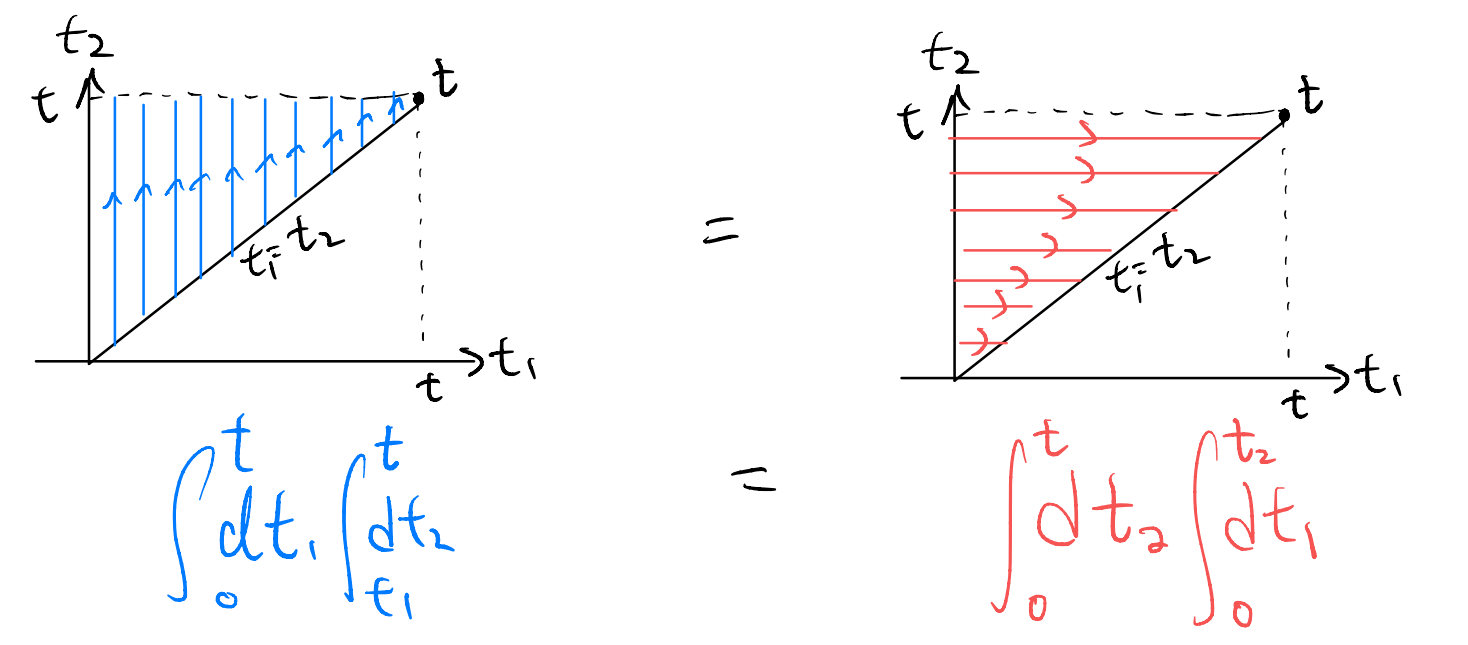
\includegraphics[width=\textwidth]{jupyterbook/data/fig/lec09-fig00.png}
\end{figure}

So we have
\begin{align*}
    &\frac{\left( -i \right) ^2}{2!}\mathcal{T} \left[ \int_0^t{dt_1\int_0^t{dt_2\hat{O}\left( t_1 \right) \hat{O}\left( t_2 \right)}} \right] \\
    =&\frac{\left( -i \right) ^2}{2!}\left\{ \int_0^t{dt_1\int_0^{t_1}{dt_2\hat{O}\left( t_1 \right) \hat{O}\left( t_2 \right)}}+{\color{red} \int_0^t{dt_2\int_0^{t_2}{dt_1{\color{black}\hat{O}\left( t_2 \right) \hat{O}\left( t_1 \right)}}}} \right\} \\
    =&\frac{\left( -i \right) ^2}{2!}\left\{ \int_0^t{dt_1\int_0^{t_1}{dt_2\hat{O}\left( t_1 \right) \hat{O}\left( t_2 \right)}}+\underset{\mathrm{relabel}\; t_1\leftrightarrow t_2}{\underbrace{{\color{red} \int_0^t{dt_1\int_0^{t_2}{dt_2{\color{black}\hat{O}\left( t_1 \right) \hat{O}\left( t_2 \right)}}}}}} \right\} \\
    =&\left( -i \right) ^2\int_0^t{dt_1\int_0^{t_1}{dt_2\hat{O}\left( t_1 \right) \hat{O}\left( t_2 \right)}}
\end{align*}
this justifies our over-counting claim (to the second order).

The argument generalizes to higher orders. For instance consider

\begin{figure}[ht]
    \centering
    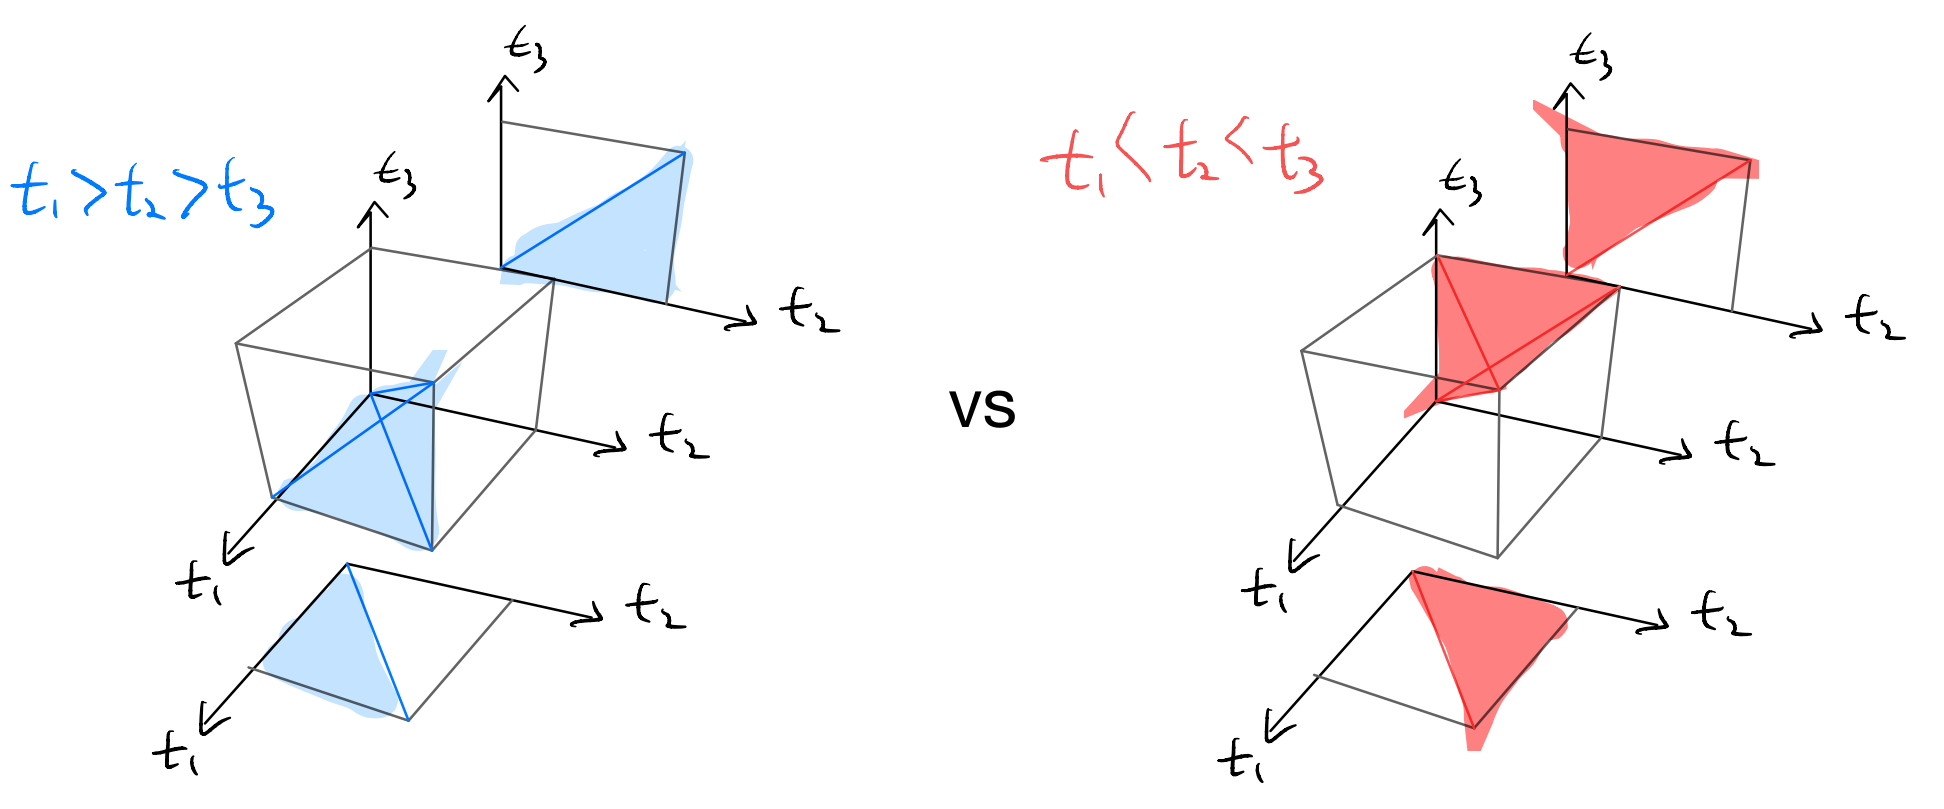
\includegraphics[width=\textwidth]{jupyterbook/data/fig/lec09-fig01.png}
\end{figure}

all these regions give the same term upon time-ordering and relabeling. All we need to do is to determine how many such regions are there. One way to see it is that each of the $3!$ permutation of $t_1,t_2,t_3$ corresponds to one region. E.g.,
\begin{align*}
    \left( t_1,t_2,t_3 \right) &\Rightarrow t_1<t_2<t_3\\
    \left( t_2,t_3,t_1 \right) &\Rightarrow t_2<t_3<t_1\\
    \left( t_1,t_3,t_2 \right) &\Rightarrow t_1<t_3<t_2\\
    \vdots &\Rightarrow \vdots
\end{align*}
More explicitly, we can also evaluate the volume of one region
\[ \int_0^t{dt_1\int_0^{t_1}{dt_2\int_0^{t_2}{dt_2\left( 1 \right)}}}=\int_0^t{dt_1\int_0^{t_1}{dt_2\left( t_2 \right)}}=\int_0^t{dt_1\left( \frac{t_{1}^{2}}{2} \right)}=\frac{t^3}{3\cdot 2}\]
and so the number of regions is $t^3/\left( \frac{t^3}{3\cdot 2} \right) =3!$.

Either of these arguments generalizes to the $n$-th order term. This establishes the equivalence of the Dyson series expansion and the time-ordered exponential.

Okay, great! With such a complicated preparation we can finally return to re-calculating the impurity Green's function (?)
\begin{align*}
    G_{11}\left( t \right) =&-i\langle \Omega |\hat{c}_{1}^{\dagger}\left( t \right) \hat{c}_1\left( 0 \right) |\Omega \rangle \\
    =&-i\langle \Omega |\underset{\mathrm{phonon}\;\mathrm{only}}{\underbrace{\mathcal{T} \left[ \exp \left( -i\int_0^t{dt'\hat{O}\left( t' \right)} \right) \right] }}\hat{c}_{1}^{\dagger}\left( 0 \right) \hat{c}_1\left( 0 \right) |\Omega \rangle \\
    &=\left( -i \right) _{100}\langle \left\{ 0_q \right\} |\mathcal{T} \left[ \exp \left( -i\int_0^t{dt'\hat{O}\left( t' \right)} \right) \right] |\left\{ 0_q \right\} \rangle _{100}
\end{align*}
where
\begin{align*}
    \hat{O}_{100}\left( t \right) =&-\varepsilon _1-\sum_q{M_{1q}\left( \hat{a}_{q}^{\left\{ 100 \right\}}\left( t \right) +\hat{a}_{q}^{\left\{ 100 \right\} \dagger}\left( t \right) -2\frac{M_{1q}}{\omega _q} \right)}\\
    =&-\varepsilon _1+2\sum_q{\frac{M_{1q}^2}{\omega _q}}-\sum_q{M_{1q}\left( \hat{a}_{q}^{\left\{ 100 \right\}}\left( t \right) +\hat{a}_{q}^{\left\{ 100 \right\} \dagger}\left( t \right) \right)}
\end{align*}
and the phonon ground state in the $\{100\}$ sector is defined by (verify!)
\[ \hat{a}_{q}^{\left\{ 100 \right\}}\left( t \right) |\left\{ 0 \right\} _q\rangle _{100}=0,\quad \forall q\]

To proceed, we make two observations:
\begin{enumerate}
    \item the constant piece in $\hat{O}(t)$ does not cause trouble, and we can just deal with it  directly to get a phase;
    \item The different phonon modes labeled by $q$ do not interfere with each other, and so we can evaluate them ``in parallel''
\end{enumerate}

This gives
\begin{align*}
    G_{11}\left( t \right) =&\left( -i \right) \exp \left[ -i\left( -\varepsilon _1+2\sum_q{\frac{M_{1q}^{2}}{\omega _q}} \right) \right] \\
    &\times \prod_q{_{100}\langle 0_q|\mathcal{T} \left[ \exp \left( iM_{1q}\int_0^t{dt'\left( \hat{a}_{q}^{\left\{ 100 \right\}}\left( t \right) +\hat{a}_{q}^{\left\{ 100 \right\} \dagger}\left( t \right) \right)} \right) \right] |0_q\rangle _{100}}
\end{align*}
Neat, but how do we evaluate this???

\section{Sub-problem: single QHO}

After massaging, we are down to evaluating the expression
\[\sim \langle 0|\mathcal{T} \left[ e^{-i\int_0^t{dt'\left( \zeta \left( t \right) \hat{a}^{\dagger}\left( t \right) +\bar{\zeta}\left( t \right) \hat{a}\left( t \right) \right)}} \right] |0\rangle \]
once for each mode labeled by $q$, with both the phonon operators and the ground state defined by the electronic configuration $\{100\}$. We have also generalized the constant $M_{iq}$ to a time-dependent function $\zeta(t)$. For simplicity, we consider here the equivalent problem of our good old single QHO. (Note: we mostly follow notations in Coleman Chapter-5 here)

how do we evaluate this? As we alluded to in the last lecture, we could employ path integral methods if we understand the time-ordered exponential as the time evolution of many small intervals; alternatively, we can try to evaluate it order-by-order if we take the Dyson-series like expansion.

Here, let us take the second route. (Check out Coleman 5.1.1 for an evaluation along the first route.)

Expanding up to first few terms,
\begin{align*}
    &\langle 0|\mathcal{T} \left[ e^{-i\int_0^t{dt'\left( \zeta \left( t \right) \hat{a}^{\dagger}\left( t \right) +\bar{\zeta}\left( t \right) \hat{a}\left( t \right) \right)}} \right] |0\rangle \\
    =&\langle 0|0\rangle -i\langle 0|\int_0^t{dt'\left( \zeta \left( t \right) \hat{a}^{\dagger}\left( t \right) +\bar{\zeta}\left( t \right) \hat{a}\left( t \right) \right)}|0\rangle \\
    &\quad +\frac{\left( -i \right) ^2}{2}\langle 0|\mathcal{T} \left[ \left( \int_0^t{dt'\left( \zeta \left( t \right) \hat{a}^{\dagger}\left( t \right) +\bar{\zeta}\left( t \right) \hat{a}\left( t \right) \right)} \right) ^2 \right] |0\rangle +\cdots \\
\end{align*}
where
\[ \langle 0|0\rangle =1\]
\[\langle 0|\hat{a}^{\dagger}\left( t \right) |0\rangle =\langle 0|\hat{a}\left( t \right) |0\rangle =0\]
\[ \Rightarrow \quad \langle 0|\int_0^t{dt'\left( \zeta \left( t \right) \hat{a}^{\dagger}\left( t \right) +\bar{\zeta}\left( t \right) \hat{a}\left( t \right) \right)}|0\rangle =0\]
and so our first nontrivial term to evaluate is
\begin{align*}
    &\frac{\left( -i \right) ^2}{2}\langle 0|\mathcal{T} \left[ \left( \int_0^t{dt'\left( \zeta \left( t \right) \hat{a}^{\dagger}\left( t \right) +\bar{\zeta}\left( t \right) \hat{a}\left( t \right) \right)} \right) ^2 \right] |0\rangle \\
    =&\frac{\left( -i \right) ^2}{2}\langle 0|\mathcal{T} \Bigl[ \int_0^t{dt_1\int_0^t{dt_2}}\zeta \left( t_1 \right) \zeta \left( t_2 \right) \hat{a}^{\dagger}\left( t_1 \right) \hat{a}^{\dagger}\left( t_2 \right) +\zeta \left( t_1 \right) \bar{\zeta}\left( t_2 \right) \hat{a}^{\dagger}\left( t_1 \right) \hat{a}\left( t_2 \right) \\
    &\qquad \left. +\bar{\zeta}\left( t_1 \right) \zeta \left( t_2 \right) \hat{a}\left( t_1 \right) \hat{a}^{\dagger}\left( t_2 \right) +\bar{\zeta}\left( t_1 \right) \bar{\zeta}\left( t_2 \right) \hat{a}\left( t_1 \right) \hat{a}\left( t_2 \right) \right] |0\rangle
\end{align*}
Noticing
\[\hat{a}\left( t \right) |0\rangle =0,\quad \langle 0|\hat{a}^{\dagger}\left( t \right) =0 \]
one may want to claim the only surviving term is
\[ \sim \langle 0|\mathcal{T} \left[ \int_0^t{dt_1\int_0^t{dt_2\bar{\zeta}\left( t_1 \right) \zeta \left( t_2 \right) \hat{a}\left( t_1 \right) \hat{a}^{\dagger}\left( t_2 \right)}} \right] |0\rangle \]
\emph{But this is wrong!} Remember, the time-ordering operator upfront implies the actual order may not be what we have written down. Instead, let us impose the time-ordering explicitly the, we do have
\begin{align*}
    &\frac{\left( -i \right) ^2}{2}\langle 0|\mathcal{T} \left[ \left( \int_0^t{dt'\left( \zeta \left( t \right) \hat{a}^{\dagger}\left( t \right) +\bar{\zeta}\left( t \right) \hat{a}\left( t \right) \right)} \right) ^2 \right] |0\rangle \\
    =&\left( -i \right) ^2\langle 0|\left[ \int_0^t{dt_1\int_0^{{\color[RGB]{240, 0, 0} t_1}}{dt_2\bar{\zeta}\left( t_1 \right) \zeta \left( t_2 \right) \hat{a}\left( t_1 \right) \hat{a}^{\dagger}\left( t_2 \right)}} \right] |0\rangle \\
    =&\left( -i \right) ^2\langle 0|\left[ \int_0^t{dt_1\int_0^{{\color[RGB]{240, 0, 0} t_1}}{dt_2\bar{\zeta}\left( t_1 \right) \zeta \left( t_2 \right) e^{-i\omega \left( t_1-t_2 \right)}}}\hat{a}\left( 0 \right) \hat{a}^{\dagger}\left( 0 \right) \right] |0\rangle \\
    =&\left( -i \right) ^2\int_0^t{dt_1\int_0^{{\color[RGB]{240, 0, 0} t_1}}{dt_2\bar{\zeta}\left( t_1 \right) \zeta \left( t_2 \right) e^{-i\omega \left( t_1-t_2 \right)}}}\langle 0|\left( \hat{a}^{\dagger}\left( 0 \right) \hat{a}\left( 0 \right) +1 \right) |0\rangle \\
    =&\left( -i \right) ^2\int_0^t{dt_1\int_0^{{\color[RGB]{240, 0, 0} t}}{dt_2{\color[RGB]{240, 0, 0} \Theta \left( t_1-t_2 \right) }e^{-i\omega \left( t_1-t_2 \right)}\bar{\zeta}\left( t_1 \right) \zeta \left( t_2 \right)}}
\end{align*}
where we have used the Heaviside step-function to restore the full integration domain for $t_2$. Let us define
\[ \mathscr{G} \left( t-t' \right) =\left( -i \right) \Theta \left( t-t' \right) e^{-i\omega \left( t-t' \right)}\]
then we see that
\[ \langle 0|\mathcal{T} \left[ e^{-i\int_0^t{dt'\left( \zeta \left( t \right) \hat{a}^{\dagger}\left( t \right) +\bar{\zeta}\left( t \right) \hat{a}\left( t \right) \right)}} \right] |0\rangle =1-i\int_0^t{dt_1\int_0^t{dt_2\bar{\zeta}\left( t_1 \right) \mathscr{G} \left( t_1-t_2 \right) \zeta \left( t_2 \right)}}+\cdots \]
where the second term is ``number'', and no ``ordering''! With a leap of faith, let us announce the answer
\[ \langle 0|\mathcal{T} \left[ e^{-i\int_0^t{dt'\left( \zeta \left( t \right) \hat{a}^{\dagger}\left( t \right) +\bar{\zeta}\left( t \right) \hat{a}\left( t \right) \right)}} \right] |0\rangle =e^{-i\int_0^t{dt_1\int_0^t{dt_2\bar{\zeta}\left( t_1 \right) \mathscr{G} \left( t_1-t_2 \right) \zeta \left( t_2 \right)}}}\]
this is kind of natural: starting with the QHO in the ground state, we perturb it by a time-dependent linear term. So if at time $t_2$ we create a quanta, let it time evolve for time $t_1-t_2$ and at time $t_1$ we annihilate it to go back to the ground state. We need to allow for all such processes happening at different times $t_1,t_2$. This ``explains'' the expression.

Of course, we haven't really proved the validity of our answer. More later.

\section{Back to the main thread}

As an indirect check of the expression we claimed, let us use it for the impurity-phonon problem:
\[ \zeta \left( t \right) =\bar{\zeta}\left( t \right) =-M_{1q}\]
\begin{align*}
    G_{11}\left( t \right) &=\left( -i \right) e^{-i\left( -\varepsilon _1+2\sum_q{\frac{M_{1q}^{2}}{\omega _q}} \right)}\prod_q{_{100}\langle 0_q|\mathcal{T} \left[ e^{iM_{1q}\int_0^t{dt'\left( \hat{a}_{q}^{\left\{ 100 \right\}}\left( t \right) +\hat{a}_{q}^{\left\{ 100 \right\} \dagger}\left( t \right) \right)}} \right] |0_q\rangle _{100}}\\
    &=\left( -i \right) e^{-i\left( -\varepsilon _1+2\sum_q{\frac{M_{1q}^{2}}{\omega _q}} \right)}\prod_q{e^{-iM_{1q}^{2}\int_0^t{dt_1\int_0^t{dt_2\mathscr{G} _q\left( t_1-t_2 \right)}}}}
\end{align*}
Evaluating the double integral
\begin{align*}
    \int_0^t{dt_1\int_0^t{dt_2\mathscr{G} _q\left( t_1-t_2 \right)}}&=-i\int_0^t{dt_1\int_0^t{dt_2\Theta \left( t_1-t_2 \right) e^{-i\omega _q\left( t_1-t_2 \right)}}}\\
    &=-i\int_0^t{dt_1\int_0^{t_1}{dt_2e^{-i\omega _q\left( t_1-t_2 \right)}}}\\
    &=-i\int_0^t{dt_1\frac{1-e^{-i\omega _qt_1}}{i\omega _q}}\\
    &=-\frac{t}{\omega _q}+\frac{e^{-i\omega _qt}-1}{-i\omega _{q}^{2}}
\end{align*}
with this we conclude (recalling $g_q=\frac{M_{1q}^{2}}{\omega _{q}^{2}}$)
\begin{align*}
    G_{11}\left( t \right) &=\left( -i \right) e^{-i\left( -\varepsilon _1+2\sum_q{\frac{M_{1q}^{2}}{\omega _q}} \right)}\prod_q{e^{i\frac{M_{1q}^{2}}{\omega _q}t}e^{\frac{M_{1q}^{2}}{\omega _{q}^{2}}\left( e^{-i\omega _qt}-1 \right)}}\\
    &=\left( -i \right) \underset{e^{i\Delta _{100}t}}{\underbrace{e^{-i\left( -\varepsilon _1+\sum_q{\frac{M_{1q}^{2}}{\omega _q}} \right) t}}}e^{\sum_q{g_q\left( e^{-i\omega _qt}-1 \right)}}
\end{align*}
This checks out! Whether this Heisenberg picture is clearer than the exact solution or not is a matter of taste: they do have a slightly different flavor nevertheless. In the exact solution, we relied heavily on the properties of the displacement operator which we discussed way back. In contrast, in the Heisenberg picture discussion, we see that we are implicitly attacking a much more general problem, namely, how to evaluate the time-evolution operator of a more general time-dependent Hamiltonian.


\chapter{lec10 20220309}

Topics

\begin{enumerate}
    \item Normal order
    \item (Static) Wick's theorem
\end{enumerate}

Goals

\begin{enumerate}
    \item Learning how to compute ground state expectation values
    \item Appreciating the what it means to be ``free'', ``Gaussian'', ``non-interacting''
\end{enumerate}

Remark: we will spend this week on a fairly technical (general) discussion.

\section{Normal order}

As discussed last time, we announced the answer
\[ \langle 0|\mathcal{T} \left[ e^{-i\int_0^t{dt'\left( \zeta \left( t' \right) \hat{a}^{\dagger}\left( t' \right) +\zeta ^*\left( t' \right) \hat{a}\left( t' \right) \right)}} \right] |0\rangle =e^{-i\int_0^t{dt_1\int_0^t{dt_2\zeta ^*\left( t_1 \right) \mathscr{G} \left( t_1-t_2 \right) \zeta \left( t_2 \right)}}}\]
\[ \mathscr{G} \left( t_1-t_2 \right) =(-i)\Theta \left( t_1-t_2 \right) e^{-i\omega \left( t_1-t_2 \right)}\]
simply by ``checking'' the lowest nontrivial term! It will make sense to demand that we do a more honest check by considering the general terms.

Let us expand the LHS
\[ \mathrm{LHS}=\sum_{n=0}{\frac{\left( -i \right) ^n}{n!}\langle 0|\mathcal{T} \left[ \left( \int_0^t{dt'\hat{\phi}\left( t' \right)} \right) ^n \right] |0\rangle}\]
\[ \hat{\phi}\left( t \right) =\zeta \left( t \right) \hat{a}^{\dagger}\left( t \right) +\zeta ^*\left( t \right) \hat{a}\left( t \right) \]
First, we notice that the only non-vanishing terms have to come with the same number of $\hat{a}\& \hat{a}^\dagger$: otherwise we leave the ground state and will have zero overlap. In particular, the odd-order terms vanish identically since there is no way to ``balance'' $\hat{a}\&\hat{a}^{\dagger}$ there. In other words,
\[ \mathrm{LHS}=\sum_{n=0}{\frac{\left( -i \right) ^{2n}}{\left( 2n \right) !}\langle 0|\mathcal{T} \left[ \left( \int_0^t{dt'\hat{\phi}\left( t' \right)} \right) ^{2n} \right] |0\rangle}\]
Let us inspect the second nontrivial term now:
\begin{align*}
    &\frac{\left( -i \right) ^4}{4!}\langle 0|\mathcal{T} \left[ \int_0^t{dt_1\int_0^t{dt_2\int_0^t{dt_3\int_0^t{dt_4\hat{\phi}\left( t_1 \right) \hat{\phi}\left( t_2 \right) \hat{\phi}\left( t_3 \right) \hat{\phi}\left( t_4 \right)}}}} \right] |0\rangle \\
    =&\frac{\left( -i \right) ^4}{4!}\langle 0|\mathcal{T} \left[ \int_0^t{dt_1\int_0^t{dt_2\int_0^t{dt_3\int_0^t{dt_4\left( \zeta \left( t_1 \right) \zeta \left( t_2 \right) \zeta ^*\left( t_3 \right) \zeta ^*\left( t_4 \right) \hat{a}^{\dagger}\left( t_1 \right) \hat{a}^{\dagger}\left( t_2 \right) \hat{a}\left( t_3 \right) \hat{a}\left( t_4 \right) \right.}}}} \right. \\
    &\qquad \left. \left. +\zeta \left( t_1 \right) \zeta ^*\left( t_2 \right) \zeta ^*\left( t_3 \right) \zeta \left( t_4 \right) \hat{a}^{\dagger}\left( t_1 \right) \hat{a}\left( t_2 \right) \hat{a}\left( t_3 \right) \hat{a}^{\dagger}\left( t_4 \right) +\cdots \right) \right] |0\rangle
\end{align*}
Ideally, we want to simplify our problem using
\[ \hat{a}\left( t \right) |0\rangle =0\]
\[ \langle 0|\hat{a}^{\dagger}\left( 0 \right) =0\]
but, as we mentioned earlier, the precise ordering of the operators is to be determined by the time-ordering, which is ``changing'' as we perform the integrals! It is then not so obvious which terms survive and which do not.

Nevertheless, it is indeed correct that we could greatly simplify the calculation if we can bring the $\hat{a}^\dagger$ to the left and $\hat{a}$ to the right. This is called the ``normal order''. The normal ordering of a time-ordered operator is the key to our evaluation, facilitated by what is usually called the Wick's theorem / lemma.

Note: ``the'' normal order is defined with respect to the ground state. When we say we bring, e.g., $\hat{a}^\dagger$ to the left and $\hat{a}$ to the right, it is implicitly assumed that our goal is to evaluate some expectation values with respect to the vacuum. Generally speaking, a different ground state calls for a different ``normal'' order.

\section{Wick's theorem}

Imagine taking the product of a string of creation and annihilation operators, e.g.,
\[ \hat{a}_1\hat{a}_{2}^{\dagger}\hat{a}_{3}^{\dagger}\hat{a}_4\hat{a}_5\hat{a}_{6}^{\dagger}\]
here, the subscripts are quite general, in that they may not only be referring to the "modes", but could also be, e.g., indicating the time as in $\hat{a}_{i}^{\dagger}=\hat{a}^{\dagger}\left( t_i \right)$. We have defined the normal order to be
\[ :\hat{a}_1\hat{a}_{2}^{\dagger}\hat{a}_{3}^{\dagger}\hat{a}_4\hat{a}_5\hat{a}_{6}^{\dagger}:=\hat{a}_{2}^{\dagger}\hat{a}_{3}^{\dagger}\hat{a}_{6}^{\dagger}\hat{a}_1\hat{a}_4\hat{a}_5\quad [\mathrm{bosonic]}\]
where the notation $:\;:$ denotes normal ordering. A natural question here is, how different is an operator $\hat{O}$ compared to its normal order $:\hat{O}:$? Relatedly, what is the ground state expectation value
\[ \langle 0|\hat{a}_1\hat{a}_{2}^{\dagger}\hat{a}_{3}^{\dagger}\hat{a}_4\hat{a}_5\hat{a}_{6}^{\dagger}|0\rangle \]
provided that it is not obviously $0$?

To develop some feeling for the problem, let's try to bring our example to the normal order
\begin{align*}
    &\hat{a}_1\hat{a}_{2}^{\dagger}\hat{a}_{3}^{\dagger}\hat{a}_4{\color{red} \hat{a}_5\hat{a}_{6}^{\dagger}}\\
    =&\hat{a}_1\hat{a}_{2}^{\dagger}\hat{a}_{3}^{\dagger}\hat{a}_4\left( \hat{a}_{6}^{\dagger}\hat{a}_5+\underset{\mathrm{c}-\mathrm{number}}{\underbrace{\left[ \hat{a}_5,\hat{a}_{6}^{\dagger} \right] }} \right) \\
    =&\hat{a}_1\hat{a}_{2}^{\dagger}\hat{a}_{3}^{\dagger}{\color{red} \hat{a}_4\hat{a}_{6}^{\dagger}}\hat{a}_5+\left[ \hat{a}_5,\hat{a}_{6}^{\dagger} \right] {\color{red} \hat{a}_1\hat{a}_{2}^{\dagger}}\hat{a}_{3}^{\dagger}\hat{a}_4\\
    =&\cdots
\end{align*}
where the operators to be exchanged are in red color.

Some observations:
\begin{enumerate}
    \item whenever we move an $\hat{a}$ pass an $\hat{a}^\dagger$, we generate two terms. One now has the ``right'' order for the two operators involved, and the other leads to a commutator multiplied to a ``shorter term'' with fewer operators involved.
    \item We can now imagine iterating the procedure. There will be a ``long string'' remaining which contains the same number of operators inside ($6$ in our example). But each of the ``short strings'' would also need to be brought to a normal order, and in doing so generate even shorter strings.
    \item Importantly, the process terminates when everything is normal ordered!
\end{enumerate}

Let's now proceed with our example in a visually more suggestive manner

\begin{figure}[ht]
    \centering
    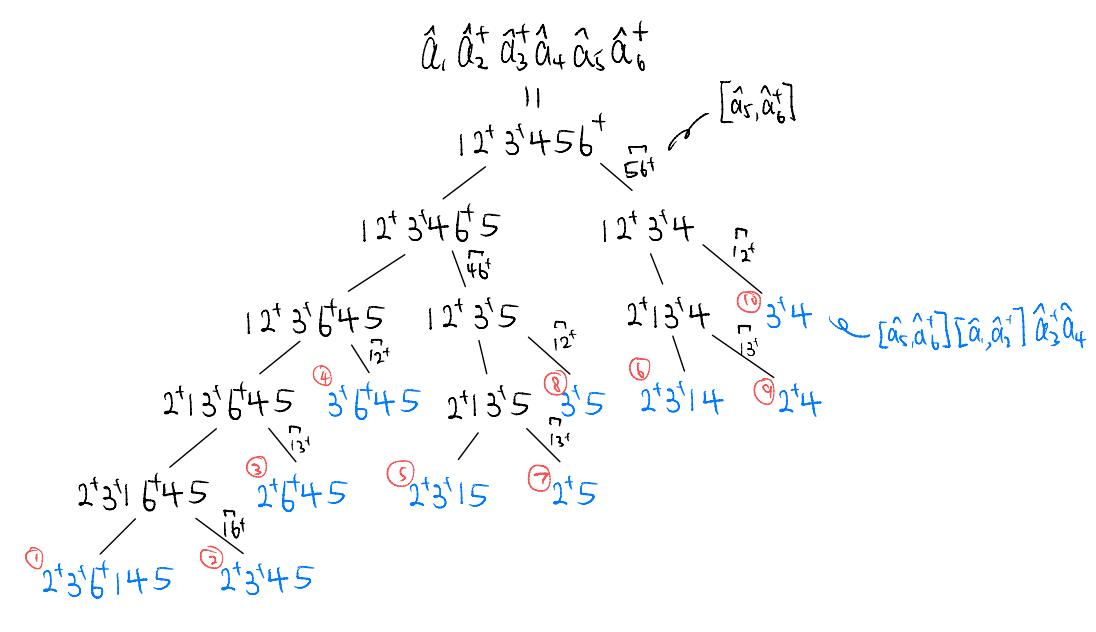
\includegraphics[width=\textwidth]{jupyterbook/data/fig/lec10-fig00.png}
\end{figure}
\newpage

we may rewrite this tree in a more conventional form
\begin{align*}
    \hat{a}_1\hat{a}_{2}^{\dagger}\hat{a}_{3}^{\dagger}\hat{a}_4\hat{a}_5\hat{a}_{6}^{\dagger}&=^{{\color{red} \text{\textcircled{1}}}}:\hat{a}_1\hat{a}_{2}^{\dagger}\hat{a}_{3}^{\dagger}\hat{a}_4\hat{a}_5\hat{a}_{6}^{\dagger}:\\
    &\quad+^{{\color{red} \text{\textcircled{2}}}}:\hat{a}_{1}^{\bullet}\hat{a}_{2}^{\dagger}\hat{a}_{3}^{\dagger}\hat{a}_4\hat{a}_5\hat{a}_{6}^{\dagger \bullet}:+^{{\color{red} \text{\textcircled{3}}}}:\hat{a}_{1}^{\bullet}\hat{a}_{2}^{\dagger}\hat{a}_{3}^{\dagger \bullet}\hat{a}_4\hat{a}_5\hat{a}_{6}^{\dagger}:\\
    &\quad+^{{\color{red} \text{\textcircled{4}}}}:\hat{a}_{1}^{\bullet}\hat{a}_{2}^{\dagger \bullet}\hat{a}_{3}^{\dagger}\hat{a}_4\hat{a}_5\hat{a}_{6}^{\dagger}:+^{{\color{red} \text{\textcircled{5}}}}:\hat{a}_1\hat{a}_{2}^{\dagger}\hat{a}_{3}^{\dagger}\hat{a}_{4}^{\bullet}\hat{a}_5\hat{a}_{6}^{\dagger \bullet}:\\
    &\quad+^{{\color{red} \text{\textcircled{6}}}}:\hat{a}_1\hat{a}_{2}^{\dagger}\hat{a}_{3}^{\dagger}\hat{a}_4\hat{a}_{5}^{\bullet}\hat{a}_{6}^{\dagger \bullet}:\\
    &\quad+^{{\color{red} \text{\textcircled{7}}}}:\hat{a}_{1}^{\bullet}\hat{a}_{2}^{\dagger}\hat{a}_{3}^{\dagger \bullet}\hat{a}_{4}^{\bullet \bullet}\hat{a}_5\hat{a}_{6}^{\dagger \bullet \bullet}:+^{{\color{red} \text{\textcircled{8}}}}:\hat{a}_{1}^{\bullet}\hat{a}_{2}^{\dagger \bullet}\hat{a}_{3}^{\dagger}\hat{a}_{4}^{\bullet \bullet}\hat{a}_5\hat{a}_{6}^{\dagger \bullet \bullet}:\\
    &\quad+^{{\color{red} \text{\textcircled{9}}}}:\hat{a}_{1}^{\bullet}\hat{a}_{2}^{\dagger}\hat{a}_{3}^{\dagger \bullet}\hat{a}_4\hat{a}_{b}^{\bullet \bullet}\hat{a}_{6}^{\dagger \bullet \bullet}:+^{{\color{red} \text{\textcircled{10}}}}:\hat{a}_{1}^{\bullet}\hat{a}_{2}^{\dagger \bullet}\hat{a}_{3}^{\dagger}\hat{a}_4\hat{a}_{b}^{\bullet \bullet}\hat{a}_{6}^{\dagger \bullet \bullet}:
\end{align*}

Notes from website builder: Since the notation for the Wick contraction used in class is hard to type in \LaTeX or HTML, here I use a different notation which is also widely used, like in Wikipedia \href{https://en.wikipedia.org/wiki/Wick\%27s\_theorem}{wiki/Wick's theorem}. Their mapping relations are
\begin{align*}
    \wick{\c a_1 a_2 a_3 \c a_4} &\Leftrightarrow a_1^\bullet a_2a_3a_4^\bullet\\
    \wick{\c1 a_1 \c2 a_2 \c2 a_3 \c1 a_4} &\Leftrightarrow a_1^\bullet a_2^{\bullet\bullet}a_3^{\bullet\bullet}a_4^\bullet
\end{align*}
In particular, by bringing it to normal order we may now conclude
\[ \langle 0|\hat{a}_1\hat{a}_{2}^{\dagger}\hat{a}_{3}^{\dagger}\hat{a}_4\hat{a}_5\hat{a}_{6}^{\dagger}|0\rangle =0\]
since no ``constants'' emerge in the ordered expansion, i.e., all terms contain an $\hat{a}_i$ at the right-most end. This is not entirely obvious without calculating! Especially, given the generality of the statement: these could be acting on the same (different) modes at the same (different) times.

Suggested sanity check: try the simple case when all operators act on the same mode at the same times, i.e., evaluate $\langle 0|\hat{a}\hat{a}^{\dagger 2}\hat{a}^2\hat{a}^{\dagger}|0\rangle$

From this exercise we can distill out a few rules:
\begin{enumerate}
    \item we can ``expand'' the original product into sum of sub-products, all of them in the normal order
    \item the coefficients of the sub-products are determined by what gets removed (pairwise) when we move the operators around, these are indicated by the symbol $a_i^\bullet a_j^\bullet$. We call them ``contractions''
    \item we only contract $\hat{a}_{i}^{\bullet}\hat{a}_{j}^{\dagger \bullet}$, Terms like $\hat{a}_{i}^{\bullet}\hat{a}_{j}^{\bullet},\hat{a}_{i}^{\dagger \bullet}\hat{a}_{j}^{\dagger \bullet},\hat{a}_{i}^{\dagger \bullet}\hat{a}_{j}^{\bullet}$ do not show up because we don't need to commute them to reach normal order
\end{enumerate}

In particular, points (2) and (3) above suggest a sharper definition of what a ``contraction'' is: it involves a pair of annihilation and creation operators, and it measures its mismatch from the normal-ordered form, i.e.,
\[ \hat{\phi}_{1}^{\bullet}\hat{\phi}_{2}^{\bullet}=\hat{\phi}_1\hat{\phi}_2-:\hat{\phi}_1\hat{\phi}_2:\]
check that, e.g.,
\[ \hat{a}_{i}^{\bullet}\hat{a}_{j}^{\dagger \bullet}=\hat{a}_i\hat{a}_{j}^{\dagger}-\hat{a}_{j}^{\dagger}\hat{a}_i=\left[ \hat{a}_i,\hat{a}_{j}^{\dagger} \right] \]
\[ \hat{a}_{i}^{\dagger \bullet}\hat{a}_{j}^{\bullet}=\hat{a}_{i}^{\dagger}\hat{a}_j-\hat{a}_{i}^{\dagger}\hat{a}_j=0\]
Importantly, our definition extends to the case when $\hat{phi}_i$ is a linear superposition of $\hat{a}_i$ and $\hat{a}_i^\dagger$, i.e., let
\[ \hat{\phi}_i=u_i\hat{a}_i+v_i\hat{a}_{i}^{\dagger}\]
then,
\begin{align*}
    \hat{\phi}_{i}^{\bullet}\hat{\phi}_{j}^{\bullet}&=\left( u_i\hat{a}_i+v_i\hat{a}_{i}^{\dagger} \right) \left( u_j\hat{a}_j+v_j\hat{a}_{j}^{\dagger} \right) -:\left( u_i\hat{a}_i+v_i\hat{a}_{i}^{\dagger} \right) \left( u_j\hat{a}_j+v_j\hat{a}_{j}^{\dagger} \right) :\\
    &=u_iv_j\hat{a}_i\hat{a}_{j}^{\dagger}-u_iv_j\hat{a}_{j}^{\dagger}\hat{a}_i\\
    &=u_iv_j\left[ \hat{a}_i,\hat{a}_{j}^{\dagger} \right]
\end{align*}
We may now state Wick's theorem more generally:
\[ \hat{\phi}_1\hat{\phi}_2\cdots \hat{\phi}_n=\sum{:\mathrm{all}\;\mathrm{possible}\;\mathrm{contractions}:}\]
here, by ``all'' we mean everything from no contraction at all, to the case of everything grouped pairwise (if $n$ is even) and contracted. As stated, it could be that many of the included terms are $0$ identically. But that's okay because it gives us a simple way to state the theorem!

Remarks:
\begin{enumerate}
    \item Contraction is not symmetric, i.e., $\hat{\phi}_{1}^{\bullet}\hat{\phi}_{2}^{\bullet}\ne \hat{\phi}_{2}^{\bullet}\hat{\phi}_{1}^{\bullet}$. E.g., $\hat{a}_{1}^{\dagger \bullet}\hat{a}_{2}^{\bullet}=0$ but $\hat{a}_{2}^{\bullet}\hat{a}_{1}^{\dagger \bullet}=\left[ \hat{a}_2,\hat{a}_{1}^{\dagger} \right] $. The order is fixed by that in the original operator we are ``expanding''
    \item Wick's theorem as stated is an operator identity.
\end{enumerate}
Evaluating vacuum expectation value is a special application. E.g., take four operators
\begin{align*}
    \hat{\phi}_1\hat{\phi}_2\hat{\phi}_3\hat{\phi}_4&=:\hat{\phi}_1\hat{\phi}_2\hat{\phi}_3\hat{\phi}_4:\\
    &\quad+\hat{\phi}_{1}^{\bullet}\hat{\phi}_{2}^{\bullet}:\hat{\phi}_3\hat{\phi}_4:+\hat{\phi}_{1}^{\bullet}\hat{\phi}_{3}^{\bullet}:\hat{\phi}_2\hat{\phi}_4:+\hat{\phi}_{1}^{\bullet}\hat{\phi}_{4}^{\bullet}:\hat{\phi}_2\hat{\phi}_3:\\
    &\quad+\hat{\phi}_{2}^{\bullet}\hat{\phi}_{2}^{\bullet}:\hat{\phi}_1\hat{\phi}_4:+\hat{\phi}_{2}^{\bullet}\hat{\phi}_{4}^{\bullet}:\hat{\phi}_1\hat{\phi}_3:+\hat{\phi}_{3}^{\bullet}\hat{\phi}_{4}^{\bullet}:\hat{\phi}_1\hat{\phi}_2:\\
    &\quad+\hat{\phi}_{1}^{\bullet}\hat{\phi}_{2}^{\bullet}\hat{\phi}_{3}^{\bullet \bullet}\hat{\phi}_{4}^{\bullet \bullet}+\hat{\phi}_{1}^{\bullet}\hat{\phi}_{3}^{\bullet}\hat{\phi}_{2}^{\bullet \bullet}\hat{\phi}_{4}^{\bullet \bullet}+\hat{\phi}_{1}^{\bullet}\hat{\phi}_{4}^{\bullet}\hat{\phi}_{2}^{\bullet \bullet}\hat{\phi}_{2}^{\bullet \bullet}
\end{align*}
which contains $C_{0}^{4}+C_{2}^{4}+\frac{1}{2}C_{2}^{4}C_{2}^{2}$ terms. If we take the expectation value
\[ \langle \Phi |\hat{\phi}_1\hat{\phi}_2\hat{\phi}_3\hat{\phi}_4|\Psi \rangle =\langle \Phi |:\hat{\phi}_1\hat{\phi}_2\hat{\phi}_3\hat{\phi}_4:|\Psi \rangle +\hat{\phi}_{1}^{\bullet}\hat{\phi}_{2}^{\bullet}\langle \Phi |:\hat{\phi}_3\hat{\phi}_4:|\Psi \rangle +\cdots \]
there isn't much of a simplification as all the terms will contribute in general. Yet if we take the vacuum expectation value (VEV)
\[ \langle 0|\hat{\phi}_1\hat{\phi}_2\hat{\phi}_3\hat{\phi}_4|0\rangle =\hat{\phi}_{1}^{\bullet}\hat{\phi}_{2}^{\bullet}\hat{\phi}_{3}^{\bullet \bullet}\hat{\phi}_{4}^{\bullet \bullet}+\hat{\phi}_{1}^{\bullet}\hat{\phi}_{3}^{\bullet}\hat{\phi}_{2}^{\bullet \bullet}\hat{\phi}_{4}^{\bullet \bullet}+\hat{\phi}_{1}^{\bullet}\hat{\phi}_{4}^{\bullet}\hat{\phi}_{2}^{\bullet \bullet}\hat{\phi}_{2}^{\bullet \bullet}\]
as all the other normal-ordered operators will annihilate the vacuum.

How many terms are there in this VEV? Consider the VEV of a string of $2n$ operators. We are asking how many ways are there to group them in pairs, noticing that
\begin{enumerate}
    \item the order within the pair is ``unimportant'', since that has to be fixed by the order in which they appeared in the original string, and
    \item once contracted, we get a c-number and it doesn't matter how we order these c-numbers.
\end{enumerate}
So, the number of terms is successively choosing two out of the remaining
\begin{align*}
    &\frac{1}{n!}C_{2}^{2n}C_{2}^{2n-2}\cdots C_{2}^{4}C_{2}^{2}\\
    =&\frac{1}{n!}\frac{\left( 2n \right) \left( 2n-1 \right)}{2}\frac{\left( 2n-2 \right) \left( 2n-3 \right)}{2}\cdots \frac{4\cdot 3}{2}\frac{2\cdot 1}{2}\\
    =&\left( 2n-1 \right) \left( 2n-3 \right) \cdots 3\cdot 1\\
    =&\left( 2n-1 \right) !!
\end{align*}
where $\frac{1}{n!}$ is the permutation of the contracted pairs.

Fun fact: you might think of the $2n$ operators as the vertices of 2 $2n$-vertex complete graph, then a term in the VEV corresponds to a perfect matching on this graph. The number of such perfecting matching is, as argued, $(2n-1)!!$.

How fast does this grow? For the first few,

\begin{table}[h!]
    \centering
    \begin{tabular}{|c|c|c|c|c|c|c|}
        \hline
        \# operators & 2 & 4 & 6 & 8 & 10 & 12\\
        \# of terms & $1!!=1$ & $3!!=3$ & $5!!=15$ & $7!!=105$ & $9!!=945$ & $11!!=10395$\\
        \hline
    \end{tabular}
\end{table}

For large $n$ we may estimate using Stirling's approximation
\[ \left( 2n-1 \right) !!\sim \left( \frac{2n}{e} \right) ^n\]
i.e., it grows super-exponentially! Combinatorial is hard... Yet, if many terms are the same then it maybe manageable

Note that the ``normal order'' is not uniquely defined. In the above, we defined it with respect to the vacuum, which instructs us to pull all the $\hat{a}_i$ to the left and $\hat{a}_i^\dagger$ to the right, as they annihilate the ket and bra correspondingly.

One could have \emph{alternative} states which are annihilated by some transformed operators, e.g., we have saw that the ``phonon vacuum'' depends on the electronic configuration in the impurity-phonon problem. One can think of it simply as a ``basis transformation'', and we can define ``alternative'' normal order with respect to such basis. The computation of expectation values then simplify in a similar manner.

These alternative normal orders correspond to alternative contractions, defined still as the the (c-number) mismatch between the operator and its normal ordered form. In fact, such contractions encode the pairwise correlation functions for the annihilation (creation) operators in the ``alternative state''. (see below) Wick's theorem then implies that, for such states for which a normal order could be defined,

\begin{displayquote}
    general correlation functions = combinatorial product and sum of up to pairwise (two-point) correlation functions.
\end{displayquote}

\noindent This is clearly very special, as generally speaking ``higher order'' correlation functions contain new data compared to the ones at ``2nd order''. The absence of such ``new data'' is the defining feature of a Gaussian distribution. Such states admitting a normal order are ``Gaussian'' in this sense.

A powerful observation about such Gaussian state $|\mathrm{GS}\rangle$ is that we do not actually need to know how to perform the normal ordering! We just need to suppose a normal order exist such that
\[ \langle GS|:\hat{\phi}_1\hat{\phi}_2\cdots \hat{\phi}_n:|GS\rangle =0\]
It then follows that
\begin{align*}
    \langle \hat{\phi}_1\hat{\phi}_2\rangle =&\langle GS|\hat{\phi}_1\hat{\phi}_2|GS\rangle ,\quad \mathrm{computable\;in\;any\;basis}\\
    =&\langle GS|:\hat{\phi}_1\hat{\phi}_2:+\hat{\phi}_{1}^{\bullet}\hat{\phi}_{2}^{\bullet}|GS\rangle \\
    =&\hat{\phi}_{1}^{\bullet}\hat{\phi}_{2}^{\bullet}
\end{align*}
In the above, the second derivation requires rotating to the right basis to literally perform the normal order. In particular, the general correlation functions can now be expressed as, e.g., for four operators
\begin{align*}
    \langle \hat{\phi}_1\hat{\phi}_2\hat{\phi}_3\hat{\phi}_4\rangle &=\hat{\phi}_{1}^{\bullet}\hat{\phi}_{2}^{\bullet}\hat{\phi}_{3}^{\bullet \bullet}\hat{\phi}_{4}^{\bullet \bullet}+\hat{\phi}_{1}^{\bullet}\hat{\phi}_{3}^{\bullet}\hat{\phi}_{2}^{\bullet \bullet}\hat{\phi}_{4}^{\bullet \bullet}+\hat{\phi}_{1}^{\bullet}\hat{\phi}_{4}^{\bullet}\hat{\phi}_{2}^{\bullet \bullet}\hat{\phi}_{2}^{\bullet \bullet}\\
    &=\langle \hat{\phi}_1\hat{\phi}_2\rangle \langle \hat{\phi}_3\hat{\phi}_4\rangle +\langle \hat{\phi}_1\hat{\phi}_3\rangle \langle \hat{\phi}_2\hat{\phi}_4\rangle +\langle \hat{\phi}_1\hat{\phi}_4\rangle \langle \hat{\phi}_2\hat{\phi}_3\rangle
\end{align*}
Looks familiar? Jumping ahead slightly, with \emph{fermionic} operators, the corresponding expression is
\[ \langle \hat{c}_{1}^{\dagger}\hat{c}_{2}^{\dagger}\hat{c}_3\hat{c}_4\rangle =\langle \hat{c}_{1}^{\dagger}\hat{c}_{2}^{\dagger}\rangle \langle \hat{c}_3\hat{c}_4\rangle +\langle \hat{c}_{1}^{\dagger}\hat{c}_4\rangle \langle \hat{c}_{2}^{\dagger}\hat{c}_3\rangle -\langle \hat{c}_{1}^{\dagger}\hat{c}_3\rangle \langle \hat{c}_{2}^{\dagger}\hat{c}_4\rangle \]
The first term is ``condensation'' which will vanish unless superconducting mean field (BdG), the second term is the direct ``Hartree'', and the third term is the exchange ``Fock'' (recalling that fermions is anti-commuting). This is the famous Hartree-Fock approximation, namely, when we approximate the actual ground state with a Gaussian state, the interaction energy consists simply of the Hartree and Fock terms. (Assuming no superconductivity)

Lastly, we note that we did not actually prove Wick's theorem. We just ``motivated'' and then ``stated'' it. For our purpose, it's probably more important to understand what it means and how to use it, than to really prove it.

Instead, let us just sketch how it could be proved
\begin{enumerate}
    \item In a ``brute force'' approach, we can establish Wick's theorem by induction. The key step is to notice what happens when we ``squeeze'' a new operator into a normal-ordered one. Supposing
    \begin{align*}
        \hat{\phi}_1:\hat{\phi}_2\cdots \hat{\phi}_n:=&:\hat{\phi}_1\hat{\phi}_2\cdots \hat{\phi}_n:+\hat{\phi}_{1}^{\bullet}\hat{\phi}_{2}^{\bullet}:\hat{\phi}_3\hat{\phi}_4\cdots \hat{\phi}_n:\\
        &\quad+\hat{\phi}_{1}^{\bullet}\hat{\phi}_{3}^{\bullet}:\hat{\phi}_2\hat{\phi}_4\cdots \hat{\phi}_n:+\cdots ++\hat{\phi}_{1}^{\bullet}\hat{\phi}_{n}^{\bullet}:\hat{\phi}_2\hat{\phi}_3\cdots \hat{\phi}_{n-1}:
    \end{align*}
    is true for $n$ operators, then we can show that it's also true for $n+1$ operators. With this established, the Wick's theorem can again be proved by induction: supposing it holds for products of up to $n$ operators, then we insert a new one from the left and all the ``new contractions'' are generated by the proposition above.
    \item Another way to prove it is to first perform a path integral with sources inserted, and then take functional derivatives. This is perhaps the more popular ``physicist'' proof. See Coleman Chapter-5 for a discussion.
    \item More interestingly still, in the ``serious QFT'' literature, there's some known connection of the Wick's theorem to what is called the ``homological perturbation lemma''. Let me know if you think you could explain that to me.
\end{enumerate}


\chapter{lec11 20220311}

Topics

\begin{enumerate}
    \item Wick's theorem and Gaussian states
    \item Wicks' theorem, time-ordering and time-ordered exponential
\end{enumerate}

Goals

\begin{enumerate}
    \item Appreciating what is means to be ``free'', ``Gaussian'', ``non-interacting'' (mean-field)
    \item Completing our explicit evaluation of the time-ordered exponential
\end{enumerate}

\section{Gaussian states}

In introducing the normal ordering, we tried to emphasize that its definition is implicitly dependent on a reference state, and so, correspondingly, the value of the contraction also depends on the reference state. We had already argued that the contraction simply equals to the ``two-point'' correlation function of the reference state. Let us show this more explicitly in a single QHO example.

To this end, let us introducing the notion of a ``squeezed state'' ( quantum optics terminology)
\[ |\zeta \rangle =\underset{\hat{S}\left( \zeta \right)}{\underbrace{e^{i\left( \zeta \hat{a}^{\dagger 2}+\zeta ^*\hat{a}^2 \right) /2}}}|0\rangle \]
We see that the squeezed state is ``rotated'' from the vacuum by a unitary, called the ``squeezed operator''
\[ \hat{S}\left( \zeta \right) =e^{i\left( \zeta \hat{a}^{\dagger 2}+\zeta ^*\hat{a}^2 \right) /2}\]

Note: our notation here differs from the usual quantum optics discussion by a factor of $i$. This is done for our convenience in what follows.

We claim the squeezed state is ``Gaussian'', and that the Wick's theorem can be applied to facilitate the evaluation of expectation values. To that end, let us first consider how the squeeze operator transform the annihilation and creation operators:
\[ \hat{S}\left( \zeta \right) \hat{a}^{\dagger}\hat{S}^{\dagger}\left( \zeta \right) =\left. e^{i\left( \zeta \hat{a}^{\dagger 2}+\zeta ^*\hat{a}^2 \right) t/2}\hat{a}^{\dagger}e^{i\left( \zeta \hat{a}^{\dagger 2}+\zeta ^*\hat{a}^2 \right) t/2} \right|_{t=1}\]
where instead of computing it directly (with BCH type formulas), we use a trick that the transformation can be interpreted as a kind of Heisenberg picture evolution with a ``squeezing Hamiltonian''
\[ i\partial _t\hat{a}^{\dagger}=\left[ \hat{a}^{\dagger},\frac{1}{2}\left( \zeta \hat{a}^{\dagger 2}+\zeta ^*\hat{a}^2 \right) \right] =-\zeta ^*\hat{a}\]
\[ \Rightarrow \quad \partial _t\left( \begin{array}{c}
	\hat{a}\\
	\hat{a}^{\dagger}\\
\end{array} \right) =i\left( \begin{matrix}
	0&		-\zeta\\
	\zeta ^*&		0\\
\end{matrix} \right) \left( \begin{array}{c}
	\hat{a}\\
	\hat{a}^{\dagger}\\
\end{array} \right)\]
\[ \Rightarrow \quad \left( \begin{array}{c}
	\hat{a}\left( t \right)\\
	\hat{a}^{\dagger}\left( t \right)\\
\end{array} \right) =\exp \left( i\left( \begin{matrix}
	0&		-\zeta\\
	\zeta ^*&		0\\
\end{matrix} \right) t \right) \left( \begin{array}{c}
	\hat{a}\left( 0 \right)\\
	\hat{a}^{\dagger}\left( 0 \right)\\
\end{array} \right)\]
For simplicity, let us further assume $\zeta=i\theta$ is purely imaginary. Then
\begin{align*}
    \exp \left( it\left( \begin{matrix}
        0&		-i\theta\\
        -i\theta&		0\\
    \end{matrix} \right) \right) &=\exp \left( \theta t\sigma _x \right) \\
    &=\sum_{n:\mathrm{even}}{\frac{1}{n!}\left( \theta t \right) ^n}+\sigma _x\sum_{n:\mathrm{odd}}{\frac{1}{n!}\left( \theta t \right) ^n}\\
    &=\cosh \left( \theta t \right) +\sigma _x\sinh \left( \theta t \right)
\end{align*}
\[ \Rightarrow \quad \left( \begin{array}{c}
	\hat{a}\left( t \right)\\
	\hat{a}^{\dagger}\left( t \right)\\
\end{array} \right) =\left( \begin{matrix}
	\cosh \left( \theta t \right)&		\sinh \left( \theta t \right)\\
	\sinh \left( \theta t \right)&		\cosh \left( \theta t \right)\\
\end{matrix} \right) \left( \begin{array}{c}
	\hat{a}\left( 0 \right)\\
	\hat{a}^{\dagger}\left( 0 \right)\\
\end{array} \right) \]
Setting $t=1$, we get
\[ \hat{S}\left( i\theta \right) \hat{a}\hat{S}^{\dagger}\left( i\theta \right) =\cosh \theta \hat{a}+\sinh \theta \hat{a}^{\dagger}\]

Note: you might recognize this as a ``Bogoliubov transformation'', usually discussed by asking what linear transformations of the bosonic operators will preserve the canonical commutation relations. We have, in fact, shown explicitly how the transformation can be achieved by the conjugate action of a unitary generated by a boson-bilinear.

With such preparation, let us verify that $|\zeta =i\theta \rangle$ is indeed a Gaussian state. For simplicity, we define
\begin{align*}
    \hat{b}&=\hat{S}\left( i\theta \right) \hat{a}\hat{S}^{\dagger}\left( i\theta \right) \\
    &=\cosh \theta \hat{a}+\sinh \theta \hat{a}^{\dagger}
\end{align*}
and the canonical commutation relation is preserved:
\[ \left[ \hat{b},\hat{b}^{\dagger} \right] =\hat{S}\left( i\theta \right) \left[ \hat{a},\hat{a}^{\dagger} \right] \hat{S}^{\dagger}\left( i\theta \right) =1\]
These are annihilation and creation operators, in that
\[ \hat{b}|i\theta \rangle =\hat{S}\left( i\theta \right) \hat{a}\hat{S}^{\dagger}\left( i\theta \right) \hat{S}\left( i\theta \right) |0\rangle =\hat{S}\left( i\theta \right) \hat{a}|0\rangle =0\]
With respect to $|i\theta \rangle$, therefore, it will be natural to define the normal order to be one in which $\hat{b}^\dagger$ is always brought to the left of $\hat{b}$.

The ``new'' normal order is then, for instance,
\begin{align*}
    :\hat{a}^{\dagger}\hat{a}:&=:\left( -\sinh \theta \hat{b}+\cosh \theta \hat{b}^{\dagger} \right) \left( \cosh \theta \hat{b}-\sinh \theta \hat{b}^{\dagger} \right) :\\
    &=-\sinh \theta \cosh \theta \hat{b}^2+\cosh ^2\theta \hat{b}^{\dagger}\hat{b}+\sinh ^2\theta {\color{red} :\hat{b}\hat{b}^{\dagger}:}-\sinh \theta \cosh \theta \hat{b}^{\dagger 2}
\end{align*}
correspondingly, the contraction becomes
\[ \hat{a}^{\dagger \bullet}\hat{a}^{\bullet}=\hat{a}^{\dagger}\hat{a}-:\hat{a}^{\dagger}\hat{a}:=\sinh ^2\theta \left[ \hat{b},\hat{b}^{\dagger} \right] =\sinh ^2\theta \]
Similarly,
\[ \hat{a}^{\bullet}\hat{a}^{\dagger \bullet}=\hat{a}\hat{a}^{\dagger}-:\hat{a}\hat{a}^{\dagger}:=\cosh ^2\theta \]
As argued, the contractions can be evaluated simply by looking at the ``two-point'' correlations. Explicitly, we have, e.g.,
\begin{align*}
    \langle i\theta |\hat{a}^{\dagger}\hat{a}|i\theta \rangle &=\langle 0|\hat{S}^{\dagger}\left( i\theta \right) \hat{a}^{\dagger}\hat{a}\hat{S}\left( i\theta \right) |0\rangle \\
    &=\langle 0|\left( -\sinh \theta \hat{a}+\cosh \theta \hat{a}^{\dagger} \right) \left( \cosh \theta \hat{a}-\sinh \theta \hat{a}^{\dagger} \right) |0\rangle \\
    &=\sinh ^2\theta \\
    &=\hat{a}^{\dagger \bullet}\hat{a}^{\bullet}
\end{align*}
Similarly, we can evaluate
\begin{align*}
    \hat{a}^{\dagger \bullet}\hat{a}^{\dagger \bullet}&=\langle i\theta |\hat{a}^{\dagger}a^{\dagger}|i\theta \rangle \\
    &=\langle 0|\left( -\sinh \theta \hat{a}+\cosh \theta \hat{a}^{\dagger} \right) ^2|0\rangle \\
    &=-\sinh \theta \cosh \theta
\end{align*}
The power of the Wick's theorem will be more apparent when we look at a longer string of operators. For instance, consider
\begin{align*}
    \langle i\theta |\left( \hat{a}^{\dagger}a \right) ^2|i\theta \rangle &=\langle i\theta |\left[ \left( -\sinh \theta \hat{a}+\cosh \theta \hat{a}^{\dagger} \right) \left( \cosh \theta \hat{a}-\sinh \theta \hat{a}^{\dagger} \right) \right] ^2|i\theta \rangle \\
    &=\langle i\theta |\left( -\sinh \theta \hat{a}+\cosh \theta \hat{a}^{\dagger} \right) \left( \cosh \theta \hat{a}-\sinh \theta \hat{a}^{\dagger} \right) \\
    &\quad\times \left( -\sinh \theta \hat{a}+\cosh \theta \hat{a}^{\dagger} \right) \left( \cosh \theta \hat{a}-\sinh \theta \hat{a}^{\dagger} \right) |i\theta \rangle \\
    &=\sinh ^2\theta \langle i\theta |\hat{a}\left( \cosh \theta \hat{a}-\sinh \theta \hat{a}^{\dagger} \right) \left( -\sinh \theta \hat{a}+\cosh \theta \hat{a}^{\dagger} \right) \hat{a}^{\dagger}|i\theta \rangle \\
    &=\sinh ^2\theta \left( \sinh ^2\theta \langle 0|\hat{a}\hat{a}^{\dagger}\hat{a}\hat{a}^{\dagger}|0\rangle +\cosh ^2\theta \langle 0|\hat{a}\hat{a}\hat{a}^{\dagger}\hat{a}^{\dagger}|0\rangle \right) \\
    &=\sinh ^2\theta \left( \sinh ^2\theta +2\cosh ^2\theta \right)
\end{align*}
Alternatively, we can write down by wick's theorem
\begin{align*}
    \langle i\theta |\left( \hat{a}^{\dagger}a \right) ^2|i\theta \rangle &=\langle \hat{a}^{\dagger}a\hat{a}^{\dagger}a\rangle \\
    &=\langle \hat{a}^{\dagger}a\rangle ^2+\langle \hat{a}^{\dagger}a\rangle \langle a\hat{a}^{\dagger}\rangle +\langle \hat{a}^{\dagger}\hat{a}^{\dagger}\rangle \langle aa\rangle \\
    &=\sinh ^4\theta +\sinh ^2\theta \cosh ^2\theta +\left( -\sinh \theta \cosh \theta \right) ^2\\
    &=\sinh ^2\theta \left( \sinh ^2\theta +2\cosh ^2\theta \right)
\end{align*}
as promised.

\section{Still remember the main thread?}

time to add time back: T-contraction

If you still remember, our goal was to establish
\[ \langle 0|\mathcal{T} \left[ e^{-i\int_0^t{dt'\left( \zeta \left( t' \right) \hat{a}^{\dagger}\left( t' \right) +\zeta ^*\left( t' \right) \hat{a}\left( t' \right) \right)}} \right] |0\rangle =e^{-i\int_0^t{dt_1\int_0^t{dt_2\zeta ^*\left( t_1 \right) \mathscr{G} \left( t_1-t_2 \right) \zeta \left( t_2 \right)}}}\]
\[ \mathscr{G} \left( t_1-t_2 \right) =-i\Theta \left( t_1-t_2 \right) e^{-i\omega \left( t_1-t_2 \right)}\]
and by noticing
\[ \mathrm{LHS}=\sum_{n=0}{\frac{\left( -i \right) ^{2n}}{\left( 2n \right) !}\langle 0|\mathcal{T} \left[ \left( \int_0^t{dt'\hat{\phi}\left( t' \right)} \right) ^n \right] |0\rangle}\]
we wandered into a (long) discussion of how to compute such VEV through Wick's theorem. Now, with Wick's theorem under our belt, we would just need to consider how that ``interacts'' with the time-ordering upfront.

To see what the new feature is, let's start with the case of two operators: $\hat{\phi}_1$ inserted at time $t_1$ and $\hat{\phi}_2$ inserted at time $t_2$
\[ \mathcal{T} \left[ \hat{\phi}_1\hat{\phi}_2 \right] =\Theta \left( t_1-t_2 \right) \hat{\phi}_1\hat{\phi}_2+\Theta \left( t_2-t_1 \right) \hat{\phi}_2\hat{\phi}_1\]
where we have used the Heaviside step function to explicitly select the correct ordering of the operators. Now we might apply Wick's theorem to the operators
\begin{align*}
    \mathcal{T} \left[ \hat{\phi}_1\hat{\phi}_2 \right] &=\Theta \left( t_1-t_2 \right) \left( :\hat{\phi}_1\hat{\phi}_2:+\hat{\phi}_{1}^{\bullet}\hat{\phi}_{2}^{\bullet} \right) +\Theta \left( t_2-t_1 \right) \left( :\hat{\phi}_2\hat{\phi}_1:+\hat{\phi}_{2}^{\bullet}\hat{\phi}_{1}^{\bullet} \right) \\
    &=:\hat{\phi}_1\hat{\phi}_2:+\Theta \left( t_1-t_2 \right) \hat{\phi}_{1}^{\bullet}\hat{\phi}_{2}^{\bullet}+\Theta \left( t_2-t_1 \right) \hat{\phi}_{2}^{\bullet}\hat{\phi}_{1}^{\bullet}
\end{align*}
let us define a ``T-contraction'' (terminology from 1710.09248):
\begin{align*}
    \overbrace{\hat{\phi}_1\hat{\phi}_2}&=\mathcal{T} \left[ \hat{\phi}_1\hat{\phi}_2 \right] -:\hat{\phi}_1\hat{\phi}_2:\\
    &=\Theta \left( t_1-t_2 \right) \hat{\phi}_{1}^{\bullet}\hat{\phi}_{2}^{\bullet}+\Theta \left( t_2-t_1 \right) \hat{\phi}_{2}^{\bullet}\hat{\phi}_{1}^{\bullet}
\end{align*}
We now claim the Wick's theorem applies in the same way for a time-ordered product simply by replacing all the contractions by T-contractions.

To illustrate this, suppose $t_2>t_3>t_1$, then
\begin{align*}
    \mathcal{T} \left[ \hat{\phi}_1\hat{\phi}_2\hat{\phi}_3 \right] &=\hat{\phi}_2\hat{\phi}_3\hat{\phi}_1\\
    &=:\hat{\phi}_1\hat{\phi}_2\hat{\phi}_3:+\hat{\phi}_{2}^{\bullet}\hat{\phi}_{3}^{\bullet}\hat{\phi}_1+\hat{\phi}_{2}^{\bullet}\hat{\phi}_{1}^{\bullet}\hat{\phi}_3+\hat{\phi}_{3}^{\bullet}\hat{\phi}_{1}^{\bullet}\hat{\phi}_2
\end{align*}
and indeed we have
\[ \overbrace{\hat{\phi}_1\hat{\phi}_2}=\Theta \left( t_1-t_2 \right) \hat{\phi}_{1}^{\bullet}\hat{\phi}_{2}^{\bullet}+\Theta \left( t_2-t_1 \right) \hat{\phi}_{2}^{\bullet}\hat{\phi}_{1}^{\bullet}=\hat{\phi}_{2}^{\bullet}\hat{\phi}_{1}^{\bullet}\]
\[ \overbrace{\hat{\phi}_2\hat{\phi}_3}=\Theta \left( t_2-t_3 \right) \hat{\phi}_{2}^{\bullet}\hat{\phi}_{3}^{\bullet}+\Theta \left( t_3-t_2 \right) \hat{\phi}_{3}^{\bullet}\hat{\phi}_{2}^{\bullet}=\hat{\phi}_{2}^{\bullet}\hat{\phi}_{3}^{\bullet}\]
\[ \overbrace{\hat{\phi}_1\hat{\phi}_3}=\Theta \left( t_1-t_3 \right) \hat{\phi}_{1}^{\bullet}\hat{\phi}_{3}^{\bullet}+\Theta \left( t_3-t_1 \right) \hat{\phi}_{3}^{\bullet}\hat{\phi}_{1}^{\bullet}=\hat{\phi}_{3}^{\bullet}\hat{\phi}_{1}^{\bullet}\]
So we have, explicitly,
\[ \mathcal{T} \left[ \hat{\phi}_1\hat{\phi}_2\hat{\phi}_3 \right] =:\hat{\phi}_1\hat{\phi}_2\hat{\phi}_3:+\overbrace{\hat{\phi}_2\hat{\phi}_3}\hat{\phi}_1+\overbrace{\hat{\phi}_2\hat{\phi}_1}\hat{\phi}_3+\overbrace{\hat{\phi}_3\hat{\phi}_1}\hat{\phi}_2\]
as claimed.

Long story short, no matter how the times are really ordered, we can apply the original Wick's theorem to the time-ordered product. However, the order of contraction might have been reversed if the two operators are swapped under the time ordering. The T-contraction takes care of such possible swapping (or not) using the Heaviside step function to toggle between the two.

In addition, we also inherit the general conclusion that the T-contraction can be computed as a ``correlation function''
\[ \langle GS|\mathcal{T} \left[ \hat{\phi}_1\hat{\phi}_2 \right] |GS\rangle =\langle GS|:\hat{\phi}_1\hat{\phi}_2:|GS\rangle +\overbrace{\hat{\phi}_1\hat{\phi}_2}=\overbrace{\hat{\phi}_1\hat{\phi}_2}\]
provided that the state is Gaussian such that there exists a definition of normal ordering with respect to that. We emphasize that we do not need to perform the actual normal ordering (basis rotation etc.) to evaluate the contraction. Its value is computed through
\[ \overbrace{\hat{\phi}_1\hat{\phi}_2}=\langle \mathcal{T} \left[ \hat{\phi}_1\hat{\phi}_2 \right] \rangle =\Theta \left( t_1-t_2 \right) \langle \hat{\phi}_1\left( t_1 \right) \hat{\phi}_2\left( t_2 \right) \rangle +\Theta \left( t_2-t_1 \right) \langle \hat{\phi}_1\left( t_2 \right) \hat{\phi}_2\left( t_1 \right) \rangle \]
where the first term is the Green's function!

\section{Time-ordered exponential meets Green's functions}

After 20 pages or so we are finally ready to evaluate the time-ordered exponential
\[ \hat{\phi}\left( t' \right) =\zeta \left( t' \right) \hat{a}^{\dagger}\left( t' \right) +\zeta ^*\left( t' \right) \hat{a}\left( t' \right) \]
\begin{align*}
    &\langle 0|\mathcal{T} \left[ e^{-i\int_0^t{dt'\hat{\phi}\left( t' \right)}} \right] |0\rangle \\
    =&\sum_{n=0}{\frac{\left( -i \right) ^{2n}}{\left( 2n \right) !}\langle 0|\mathcal{T} \left[ \int_0^t{dt_1\int_0^t{dt_2\cdots \int_0^t{dt_n\hat{\phi}\left( t_1 \right) \hat{\phi}\left( t_2 \right) \cdots \hat{\phi}\left( t_{2n} \right)}}} \right] |0\rangle}\\
    =&\sum_{n=0}{\frac{\left( -i \right) ^{2n}}{\left( 2n \right) !}\int_0^t{dt_1\int_0^t{dt_2\cdots \int_0^t{dt_n{\color{red} \langle 0|\mathcal{T} \left[ \hat{\phi}\left( t_1 \right) \hat{\phi}\left( t_2 \right) \cdots \hat{\phi}\left( t_{2n} \right) \right] |0\rangle }}}}}
\end{align*}
\begin{align*}
    &{\color{red} \langle 0|\mathcal{T} \left[ \hat{\phi}\left( t_1 \right) \hat{\phi}\left( t_2 \right) \cdots \hat{\phi}\left( t_{2n} \right) \right] |0\rangle }\\
    =&\overbrace{\hat{\phi}\left( t_1 \right) \hat{\phi}\left( t_2 \right) }\overbrace{\hat{\phi}\left( t_3 \right) \hat{\phi}\left( t_4 \right) }\cdots \overbrace{\hat{\phi}\left( t_{2n-1} \right) \hat{\phi}\left( t_{2n} \right) }\\
    &\quad+\overbrace{\hat{\phi}\left( t_1 \right) \hat{\phi}\left( t_3 \right) }\overbrace{\hat{\phi}\left( t_2 \right) \hat{\phi}\left( t_4 \right) }\cdots \overbrace{\hat{\phi}\left( t_{2n-1} \right) \hat{\phi}\left( t_{2n} \right) }\\
    &\quad+\cdots ;\quad \left( 2n-1 \right) !! \mathrm{terms}
\end{align*}
Now, we evaluate
\begin{align*}
    &\overbrace{\hat{\phi}\left( t_1 \right) \hat{\phi}\left( t_2 \right) }\\
    =&\langle 0|\mathcal{T} \left[ \hat{\phi}\left( t_1 \right) \hat{\phi}\left( t_2 \right) \right] |0\rangle \\
    =&\Theta \left( t_1-t_2 \right) \langle 0|\left( \zeta \left( t_1 \right) \hat{a}^{\dagger}\left( t_1 \right) +\zeta ^*\left( t_1 \right) \hat{a}\left( t_1 \right) \right)\\
    &\quad \times \left( \zeta \left( t_2 \right) \hat{a}^{\dagger}\left( t_2 \right) +\zeta ^*\left( t_2 \right) \hat{a}\left( t_2 \right) \right) |0\rangle +\left( t_1\leftrightarrow t_2 \right) \\
    =&\Theta \left( t_1-t_2 \right) \zeta ^*\left( t_1 \right) \zeta \left( t_2 \right) \langle 0|\hat{a}e^{-i\omega t_1}\hat{a}^{\dagger}e^{i\omega t_2}|0\rangle +\left( t_1\leftrightarrow t_2 \right) \\
    =&\Theta \left( t_1-t_2 \right) \zeta ^*\left( t_1 \right) \zeta \left( t_2 \right) e^{-i\omega \left( t_1-t_2 \right)}+\left( t_1\leftrightarrow t_2 \right)
\end{align*}
We defined
\[ \mathscr{G} \left( t_1-t_2 \right) =\left( -i \right) \Theta \left( t_1-t_2 \right) e^{-i\omega \left( t_1-t_2 \right)}\]
\begin{align*}
    \Rightarrow \quad &\int_0^t{dt_1\int_0^t{dt_2\overbrace{\hat{\phi}\left( t_1 \right) \hat{\phi}\left( t_2 \right) }}}\\
    =&\frac{1}{\left( -i \right)}\int_0^t{dt_1\int_0^t{dt_2\zeta ^*\left( t_1 \right) \mathscr{G} \left( t_1-t_2 \right) \zeta \left( t_2 \right)}}+\left( t_1\leftrightarrow t_2 \right) \\
    =&\left( 2i \right) \int_0^t{dt_1\int_0^t{dt_2\zeta ^*\left( t_1 \right) \mathscr{G} \left( t_1-t_2 \right) \zeta \left( t_2 \right)}}
\end{align*}
In addition, all the other full contractions generated by Wick's theorem correspond to exactly the same expression but with some relabeling of the time indices. In other words, all the $(2n-1)!!$ terms evaluate to the same answer. We can finally write down
\begin{align*}
    &\langle 0|\mathcal{T} \left[ e^{-i\int_0^t{dt'\left( \zeta \left( t' \right) \hat{a}^{\dagger}\left( t' \right) +\zeta ^*\left( t' \right) \hat{a}\left( t' \right) \right)}} \right] |0\rangle \\
    =&\sum_{n=0}{\frac{\left( -i \right) ^{2n}}{\left( 2n \right) !}\left( 2i \right) ^n\left[ \int_0^t{dt_1\int_0^t{dt_2\zeta ^*\left( t_1 \right) \mathscr{G} \left( t_1-t_2 \right) \zeta \left( t_2 \right)}} \right] ^n\times \left( 2n-1 \right) !!}\\
    =&\sum_{n=0}{\left( -i \right) ^n\frac{2^n\left( 2n-1 \right) !!}{\left( 2n \right) !}\left[ \int_0^t{dt_1\int_0^t{dt_2\zeta ^*\left( t_1 \right) \mathscr{G} \left( t_1-t_2 \right) \zeta \left( t_2 \right)}} \right] ^n}\\
    =&\exp \left( -i\int_0^t{dt_1\int_0^t{dt_2\zeta ^*\left( t_1 \right) \mathscr{G} \left( t_1-t_2 \right) \zeta \left( t_2 \right)}} \right)
\end{align*}
where we have used
\[ \frac{2^n\left( 2n-1 \right) !!}{\left( 2n \right) !}=\frac{1}{n!}\]
Finally, we've established this honestly! (Again, see Coleman 5.1.1 if you want an alternative discussion)

Notes:

\begin{enumerate}
    \item (For the QFT gurus in the audience) You may think that our approach to Wick's theorem is unnecessarily complicated: isn't it just taking functional derivative on the free-field S-matrix? You are right, but note that our ``operator'' form (as an identity) is actually a bit stronger than a relation between correlation and Green's function.
    \item Our calculation above actually works more generally: we simply define
    \[ G\left( x,x';t,t' \right) =\langle \Omega |\mathcal{T} \left[ \hat{\phi}_x\left( t \right) \hat{\phi}_{x'}\left( t' \right) \right] |\Omega \rangle \]
    where $\hat{\phi}_x\left( t \right) ,\hat{\phi}_{x'}\left( t' \right)$ are the ``field operators'' creating or annihilating particles at different points in space-time, and denotes the many-body ground state which, generally speaking, is not Gaussian = free (why should it be?). We call this the ``one-particle'' Green's function.
\end{enumerate}

The goal of a perturbation theory is to derive an expansion of the actual quantities in terms of those for an unperturbed problem. A useful unperturbed problem is one for which the same set of quantities could be computed. (Always attack a hard problem starting from an easier starting point, and work your way there!) In our context, we take the Gaussian theory as the starting point, and the perturbative expansions are then organized and computed in terms of ``Feynman diagrams''.


\chapter{Lec12 20220316}

Topics

\begin{enumerate}
    \item Propagators
    \item Frequency space, contours and real-time Green functions
\end{enumerate}

Goals

\begin{enumerate}
    \item Arriving at a more systematic treatment of the various notion of Green's functions we have encountered
\end{enumerate}

\section{Bare phonon propagator}

Let us revisit the free-phonon problem again from this lens of T-contractions and correlation functions. Consider again
\[ \hat{H}=\sum_q{\omega _q\hat{a}_{q}^{\dagger}\hat{a}_q}\]
where for simplicity we have restricted ourselves to a single ``branch'' and so suppressed any additional indices which might be attached to the phonon operators aside from the (crystal) momentum $q$.

In the real space, the phonon operators are related to the actual position (deviation) operators of the atoms through
\[ \hat{\phi}_r=\frac{1}{\sqrt{V}}\sum_q{e^{-iqr}\left( \frac{\hat{a}_q+\hat{a}_{-q}^{\dagger}}{\sqrt{2m\omega _q}} \right)}=\frac{1}{\sqrt{V}}\sum_q{e^{-iqr}\hat{\phi}_q}\]
In the Heisenberg picture, the phonon operators evolve in time according to
\[ i\partial _t\hat{a}_q\left( t \right) =\left[ \hat{a}_q\left( t \right) ,\omega _q\hat{a}_{q}^{\dagger}\left( t \right) \hat{a}_q\left( t \right) \right] =\omega _q\hat{a}_q\left( t \right) \]
\[ \hat{a}_q\left( t \right) =\hat{a}_q\left( 0 \right) e^{-i\omega _qt}\]
And we may evaluate the one-particle Green's function with respect to the phonon vacuum (superscript $t$ emphasize it corresponds to the time-ordered two-point function)
\begin{align*}
    G^t\left( r,r';t,t' \right) &=-i\langle \mathrm{vac}|\mathcal{T} \left[ \hat{\phi}_r\left( t \right) \hat{\phi}_{r'}\left( t' \right) \right] |\mathrm{vac}\rangle \\
    &=\frac{-i}{V}\sum_{qq'}{\frac{e^{-iq\cdot r}e^{-iq'\cdot r'}}{2m\sqrt{\omega _q\omega _{q'}}}\langle \mathrm{vac}|\mathcal{T} \left[ \overset{\hat{\phi}_q\left( t \right)}{\overbrace{\left( \hat{a}_q\left( t \right) +\hat{a}_{-q}^{\dagger}\left( t \right) \right) }}\left( \hat{a}_{q'}\left( t' \right) +\hat{a}_{-q'}^{\dagger}\left( t' \right) \right) \right] |\mathrm{vac}\rangle}\\
    & \qquad\left( q=-q' \right) \\
    &=\frac{-i}{V}\sum_q{\frac{e^{-iq\cdot \left( r-r' \right)}}{2m\omega _q}\langle \mathrm{vac}|\mathcal{T} \left[ \hat{a}_q\left( t \right) \hat{a}_{q}^{\dagger}\left( t' \right) +\hat{a}_{-q}^{\dagger}\left( t \right) \hat{a}_{-q}\left( t' \right) \right] |\mathrm{vac}\rangle}
\end{align*}
\begin{align*}
    \Rightarrow \quad \langle \mathrm{vac}|\mathcal{T} \left[ \hat{a}_q\left( t \right) \hat{a}_{q}^{\dagger}\left( t' \right) \right] |\mathrm{vac}\rangle &=\Theta \left( t-t' \right) \langle \mathrm{vac}|\hat{a}_q\left( t \right) \hat{a}_{q}^{\dagger}\left( t' \right) |\mathrm{vac}\rangle \\
    &=\Theta \left( t-t' \right) e^{-i\omega _q\left( t-t' \right)}
\end{align*}
\[ \Rightarrow \quad \,\,G^t\left( r,r';t,t' \right) =\frac{-i}{V}\sum_q{\frac{e^{-iq\cdot \left( r-r' \right)}}{2m\omega _q}\left( \Theta \left( t-t' \right) e^{-i\omega _q\left( t-t' \right)}+\Theta \left( t'-t \right) e^{-i\omega _{-q}\left( t'-t \right)} \right)}\]
which depends only on $r-r'$ and $t-t'$
\[ G^t\left( r,t \right) =\frac{-i}{V}\sum_q{\frac{e^{-iq\cdot r}}{2m\omega _q}\left( \Theta \left( t \right) e^{-i\omega _qt}+\Theta \left( -t \right) e^{i\omega _{-q}t} \right)}\]
The translation invariance, exposed in the fact that the two-point function depends only on $r-r'$ implies $q$ is a good quantum number and it is natural to Fourier transform
\begin{align*}
    G^t\left( q,t \right) &=\sum_r{e^{iq\cdot r}G^t\left( r,t \right)}\\
    &=\frac{-i}{2m\omega _q}\left( \Theta \left( t \right) e^{-i\omega _qt}+\Theta \left( -t \right) e^{i\omega _{-q}t} \right)
\end{align*}
We may further Fourier transform to the frequency space, using our ``exponential damping trick''
\begin{align*}
    G^t\left( q,\omega \right) &=\lim_{\eta \rightarrow 0^+} \int_{-\infty}^{\infty}{dtG^t\left( q,t \right) e^{i\omega t-\eta \left| t \right|}}\\
    &=\frac{-i}{2m\omega _q}\lim_{\eta \rightarrow 0^+} \left( \int_0^{\infty}{dte^{i\left( \omega -\omega _q+i\eta \right) t}}+\int_{-\infty}^0{dte^{i\left( \omega +\omega _q+i\eta \right) t}} \right) \\
    &=\frac{-i}{2m\omega _q}\lim_{\eta \rightarrow 0^+} \left( \frac{0-1}{i\left( \omega -\omega _q+i\eta \right)}+\frac{1-0}{i\left( \omega +\omega _q+i\eta \right)} \right) \\
    &=\frac{1}{2m\omega _q}\lim_{\eta \rightarrow 0^+} \left( \frac{1}{\omega -\omega _q+i\eta}-\frac{1}{\omega +\omega _q+i\eta} \right) \\
    &=\frac{1}{2m\omega _q}\lim_{\eta \rightarrow 0^+} \frac{2\omega _q}{\omega ^2-\left( \omega _q-i\eta \right) ^2}
\end{align*}
This is called the free/bare phonon ``propagator''. It is customary to denote it by $D$ (instead of $G$), since in an electron-phonon problem one might want to reserve $G$ for the electrons.

\section{Contours, Green's function, Feynman's $i\epsilon$ prescription}

Going from the real-time to frequency space, we have used an exponential damping term to regulate the oscillatory integral extending to $t\to\pm\infty$. In particular, the sign of the damping depends on the sign of $t$. We first introduced such tricks by alluding to the physical reality that our system cannot possibly exist all the way up to $t\to\pm\infty$ anyway, and so it is natural to regulate the integral by damping it off. Here, we provide an alternative way to make sense of such treatment.

We first notice that the (bare) phonon Green's function $D^t(q,\omega)$, viewed as a complex function, contains two poles
\[ D^+\left( q,\omega \right) =\frac{1}{2m\omega _q}\lim_{\eta \rightarrow 0^+} \left( \frac{1}{\omega -\omega _q+i\eta}-\frac{1}{\omega +\omega _q+i\eta} \right) \]
which are infinitesimally displaced from the real line.

\begin{figure}[ht]
    \centering
    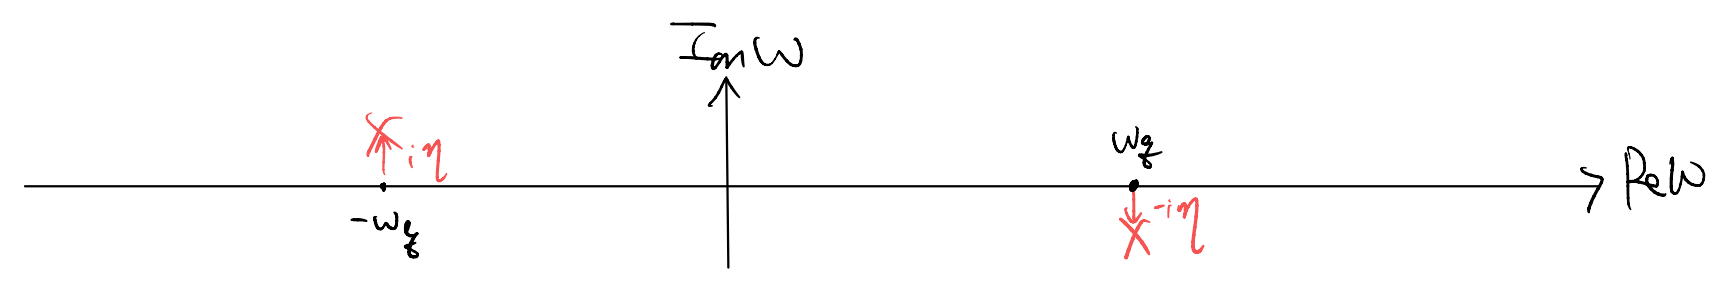
\includegraphics[width=\textwidth]{jupyterbook/data/fig/lec12-fig00.png}
\end{figure}

Now, imagine Fourier transforming back to the real time, which calls for an integral along the real line, with the two poles approaching our integration contour, Such integrals could alternatively be computed by trading the $\pm i\eta$ with an infinitesimal deformation of the integration contour.
\begin{figure}[ht]
    \centering
    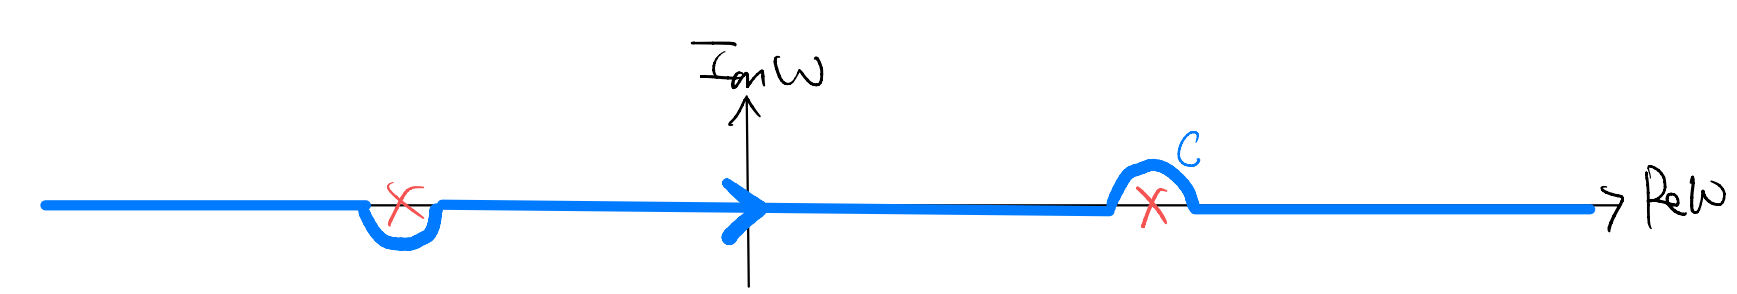
\includegraphics[width=\textwidth]{jupyterbook/data/fig/lec12-fig01.png}
\end{figure}
As a sanity check, let us verify that we could indeed go back to the real-time Green's function by performing such contour integrals. Consider
\[ \frac{1}{2m\omega _q}\int_C{\frac{d\omega}{2\pi}\left( \frac{1}{\omega -\omega _q}-\frac{1}{\omega +\omega _q} \right)}e^{-i\omega t}\]
Notice we have dropped the $\pm i\eta$, with the corresponding information encoded in how the contour $C$ is specified.

One could evaluate this integral honestly, by splitting the contour $C$ into $5$ segments: three straight lines and two semi-circles. As the deformation is only infinitesimal, the ``straight line'' integrals return  the Cauchy principal value whereas the ``semi-circles'' give half of the residues. In addition, for the principal part one ultimately gets the Dirichlet sinc integral, which gives $\sim e^{\pm i\omega_q t}(i\pi \mathrm{sgn}(t))$. Combined with the partial residues, one does get back the original time-ordered real-time Green's function.

Instead of going through the details of the steps sketeched above, let's use the usual ``physicist's argument'' to evaluate the integral. The main idea is to use the residue theorem, which states that (loosely) power series make sense except at the singularities (i.e., poles)
\[ \oint{\gamma}{d\zeta f\left( \zeta \right)}=2\pi i\sum{\mathrm{Res}\left( f,a_k \right)}\]
\begin{figure}[ht]
    \centering
    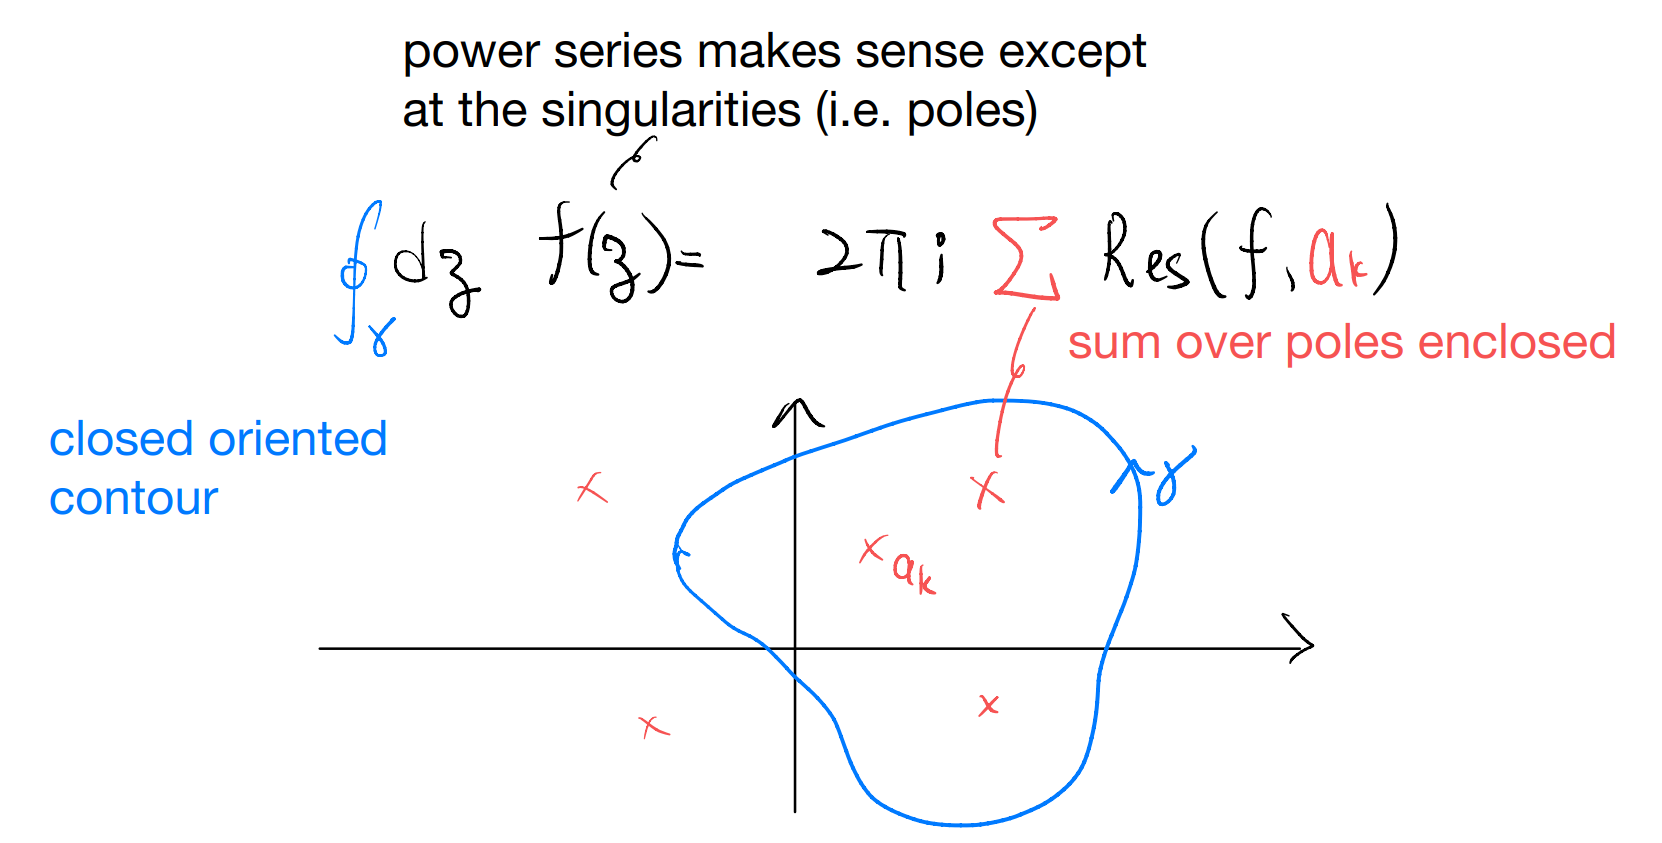
\includegraphics[width=\textwidth]{jupyterbook/data/fig/lec12-fig02.png}
\end{figure}
and for a meromorphic function with a simple pole, taking the form
\begin{align*}
    f\left( \zeta \right) &=\frac{g\left( \zeta \right)}{\zeta -a_k}=\frac{\sum_{n=0}{g_n\left( \zeta -a_k \right) ^n}}{\zeta -a_k}\\
    &=\frac{g_0}{\zeta -a_k}+g_1+g_2\left( \zeta -a_k \right) +\cdots
\end{align*}
the residue is simply the coefficient $g_0$.

Now, back to our problem: to take advantage of the residue theorem we would want to ``close'' our contour. The natural choice will be to complete it with an arc which we send off to infinity, e.g.,
\begin{figure}[ht]
    \centering
    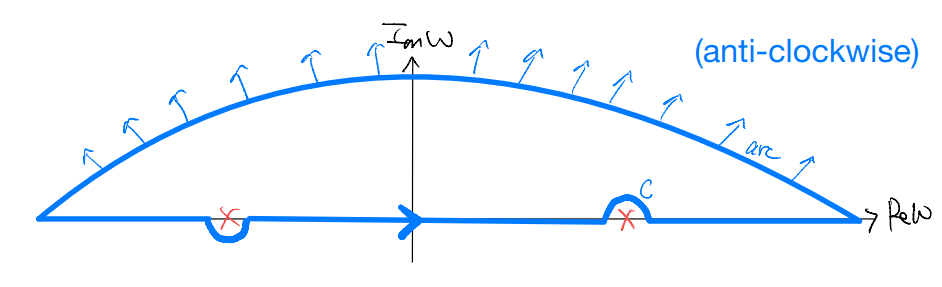
\includegraphics[width=\textwidth]{jupyterbook/data/fig/lec12-fig03.png}
\end{figure}
We then see that, by the residue theorem, only one of the poles contribute:
\begin{align*}
    \int_{C+arc}{\frac{d\omega}{2\pi}D\left( q,\omega \right) e^{-i\omega t}}&=\frac{1}{2m\omega _q}\frac{2\pi i}{2\pi}\mathrm{Res}\left( \frac{-e^{-i\omega t}}{\omega +\omega _q},\omega -\omega _q \right) \\
    &=\frac{-i}{2m\omega _q}e^{i\omega _qt}
\end{align*}
\[ \Rightarrow \quad \int_C{\frac{d\omega}{2\pi}D\left( q,\omega \right) e^{-i\omega t}}=\frac{-i}{2m\omega _q}e^{i\omega _qt}-\int_{arc}{\frac{d\omega}{2\pi}D\left( q,\omega \right) e^{-i\omega t}}\]
almost! But we need to know what is the contribution from the arc. In what we considered above, we let $\omega$ go to infinity on the upper complex plane. In other words, we consider
\[ \mathrm{Im}\left( \omega \right) \rightarrow +\infty \]
as such, in the integrand we have
\[ e^{-i\omega t}=e^{-i\mathrm{Re}\left( \omega \right) t}e^{\mathrm{Im}\left( \omega \right) t}\]
and it is well-behaved (and exponentially suppressed) only if we have $t<0$ to start with. Provided $t<0$, the arc contribution goes to zero as the integrand is now exponentially suppressed. This gives
\[ \int_C{\frac{d\omega}{2\pi}D\left( q,\omega \right) e^{-i\omega t}}=\frac{-i}{2m\omega _q}e^{i\omega _qt},\quad t<0\]
Now, to obtain the result for $t>0$, we should consider the alternative way of closing off our contour (clockwise)
\begin{figure}[ht]
    \centering
    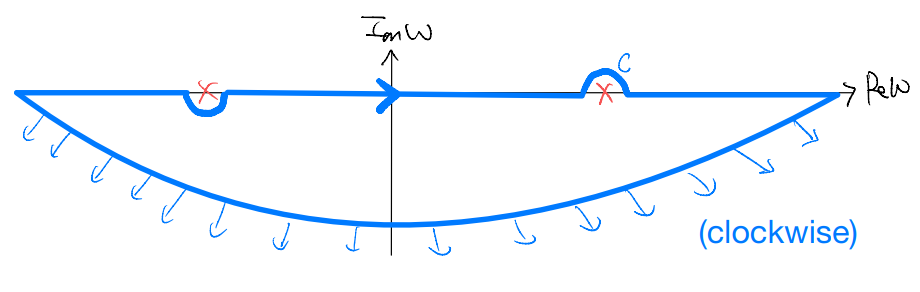
\includegraphics[width=\textwidth]{jupyterbook/data/fig/lec12-fig04.png}
\end{figure}
which now encloses the other pole at $\omega=\omega_q$. The same calculation as before then gives
\begin{align*}
    \int_C{\frac{d\omega}{2\pi}D\left( q,\omega \right) e^{-i\omega t}}&=\frac{-1}{2m\omega _q}\frac{2\pi i}{2\pi}\mathrm{Res}\left( \frac{e^{-i\omega t}}{\omega -\omega _q},\omega =\omega _q \right) -\int_{arc}{\frac{d\omega}{2\pi}D\left( q,\omega \right) e^{-i\omega t}}\\
    &=\frac{-i}{2m\omega _q}e^{-i\omega _qt},\quad t>0
\end{align*}
We may then combine the two cases into
\[ \int_C{\frac{d\omega}{2\pi}D\left( q,\omega \right) e^{-i\omega t}}=\frac{-i}{2m\omega _q}\left( \Theta \left( t \right) e^{-i\omega _qt}+\Theta \left( -t \right) e^{i\omega _qt} \right) =D^t\left( q,t \right) \]
as promised. We note in passing that, this is also commonly referred to as the (Feynman) ``propagator''.

Such time-ordered correlation function shows up in perturbation expansion (Feynman diagrams etc.), and we will see that they can be interpreted as the free propagation of phonons, whence the name.

One may wonder what's the significance of undergoing such a lengthy discussion in order to simply Fourier transform back to the real time. The catch is that, in the calculation above, it will be natural to consider alternative contours which circumvent the two poles in some other means. For instance, consider the contour
\begin{figure}[ht]
    \centering
    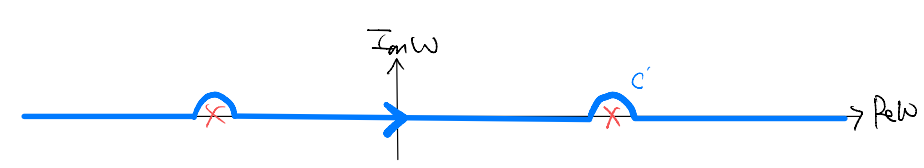
\includegraphics[width=\textwidth]{jupyterbook/data/fig/lec12-fig05.png}
\end{figure}
It doesn't encircle any poles if we complete it in the upper complex plane (Fourier transform with $t<0$), and enclose both poles when we complete in the lower complex plane. This gives
\[ \int_{C'}{\frac{d\omega}{2\pi}D\left( q,\omega \right) e^{-i\omega t}}=-i\Theta \left( t \right) \left( e^{-i\omega _qt}-e^{i\omega _qt} \right) =-2\Theta \left( t \right) \sin \left( \omega _qt \right)\]
What is the process corresponding to this real-time Green's function? Notice that, what we have changed is really the integration around the pole at $\omega=-\omega_q$. First consider
\begin{figure}[ht]
    \centering
    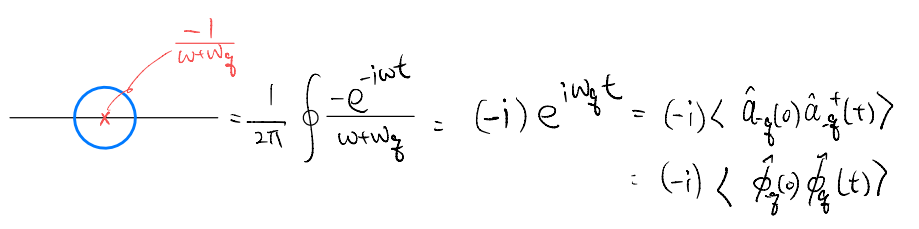
\includegraphics[width=\textwidth]{jupyterbook/data/fig/lec12-fig06.png}
\end{figure}
\[ \oint{\frac{d\omega}{2\pi}\frac{-e^{-i\omega t}}{\omega +\omega _q}}=\left( -i \right) e^{i\omega _qt}=\left( -i \right) \left< \hat{a}_{-q}\left( 0 \right) \hat{a}_{-q}^{\dagger}\left( t \right) \right> =\left( -i \right) \left< \hat{\phi}_{-q}\left( 0 \right) \hat{\phi}_{q}^{\dagger}\left( t \right) \right> \]
Now, we can compare the two contours considered
\begin{figure}[ht]
    \centering
    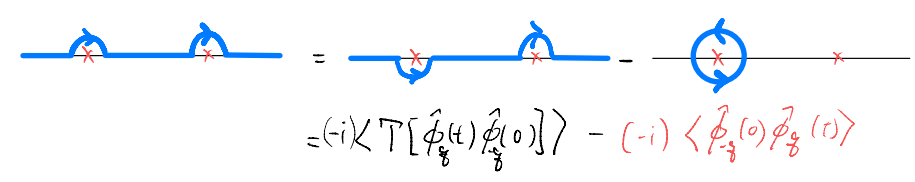
\includegraphics[width=\textwidth]{jupyterbook/data/fig/lec12-fig07.png}
\end{figure}
\begin{align*}
    &\left( -i \right) \left< \mathcal{T} \left[ \hat{\phi}_q\left( t \right) \hat{\phi}_{-q}\left( 0 \right) \right] \right> -\left( -i \right) \left< \mathcal{T} \left[ \hat{\phi}_{-q}\left( 0 \right) \hat{\phi}_q\left( t \right) \right] \right> \\
    =&\left( -i \right) \Theta \left( t \right) \left< \hat{\phi}_q\left( t \right) \hat{\phi}_{-q}\left( 0 \right) \right> +\left( -i \right) \Theta \left( -t \right) \left< \hat{\phi}_{-q}\left( 0 \right) \hat{\phi}_q\left( t \right) \right> \\
    &\quad -\left( -i \right) \Theta \left( t \right) \left< \hat{\phi}_{-q}\left( 0 \right) \hat{\phi}_q\left( t \right) \right> -\left( -i \right) \Theta \left( -t \right) \left< \hat{\phi}_{-q}\left( 0 \right) \hat{\phi}_q\left( t \right) \right> \\
    =&\left( -i \right) \Theta \left( t \right) \left< \left[ \hat{\phi}_{-q}\left( 0 \right) ,\hat{\phi}_q\left( t \right) \right] \right>
\end{align*}
i.e., it is the expectation value of a commutator with time $t>0$.

By closing the contour on the lower complex plane, our real-time Green's function is non-vanishing only for $t>0$, which suggests a kind of causality, in the sense that we only allow time to move ``forward'' but not backward. Indeed, this is known as the causal / retarded Green's function of the phonons, and is closely related to the response of a system when we perturb it (and the system can only respond after we perturb it, by causality). More later.

Lastly, a comment on contours vs $i\eta$: in the above, we see that the same frequency space Green's function, combined with different contour prescription (for avoiding the singularities on the real axis), gives rise to different real-time Green's functions. Yet, we also argued (heuristically) that, the contour prescription can be understood simply by the small shifts $\pm i\eta$ kicking the poles off the real axis. So, instead of specifying different contours, we can also stick with the real line (and leave the ``arc'' part implicit, dependent on the sign of time), and instead assign the $\pm i\eta$ as the definition for different Green's functions.

This latter perspective is perhaps more popular among physicists, and this is called ``Feynman's $i\epsilon$ prescription''. (Probably he used $\epsilon$ for what we denoted by $\eta$ here.)

A particularly important ``pole structure'' for our next topic (linear response) is as follows:
\begin{figure}[ht]
    \centering
    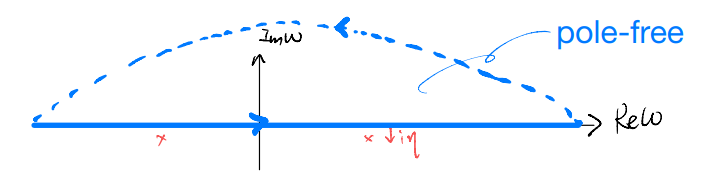
\includegraphics[width=\textwidth]{jupyterbook/data/fig/lec12-fig08.png}
\end{figure}
where the $i\eta$ displaces the poles to the lower complex plane. This corresponds to the contours we considered just now for the phonons:
\begin{figure}[ht]
    \centering
    
\includegraphics[width=\textwidth]{jupyterbook/data/fig/lec12-fig09.png}
\end{figure}
When we Fourier transform back to real time, the integral vanishes when we close the contour on the upper complex plane, i.e., the only contribution comes from $t>0$, and the real-time Green's function is ``retarded'' in the sense that
\[ G_{\mathrm{ret}}\left( t,t' \right) \propto \Theta \left( t-t' \right) \]
To summarize, when we consider Fourier transform back to real time
\begin{align*}
    f\left( t \right) &=\int_{-\infty}^{\infty}{\frac{d\omega}{2\pi}f\left( \omega \right) e^{-i\omega t}}\\
    &=\int_{-\infty}^{\infty}{\frac{d\mathrm{Re}\left( \omega \right)}{2\pi}f\left( \omega \right) e^{-i\mathrm{Re}\left( \omega \right) t}e^{\mathrm{Im}\left( \omega \right) t}}\\
    &\sim \begin{cases}
        \Theta \left( t \right) ,\quad t>0\\
        \Theta \left( -t \right) ,\quad t<0\\
    \end{cases}
\end{align*}
\begin{figure}[ht]
    \centering
    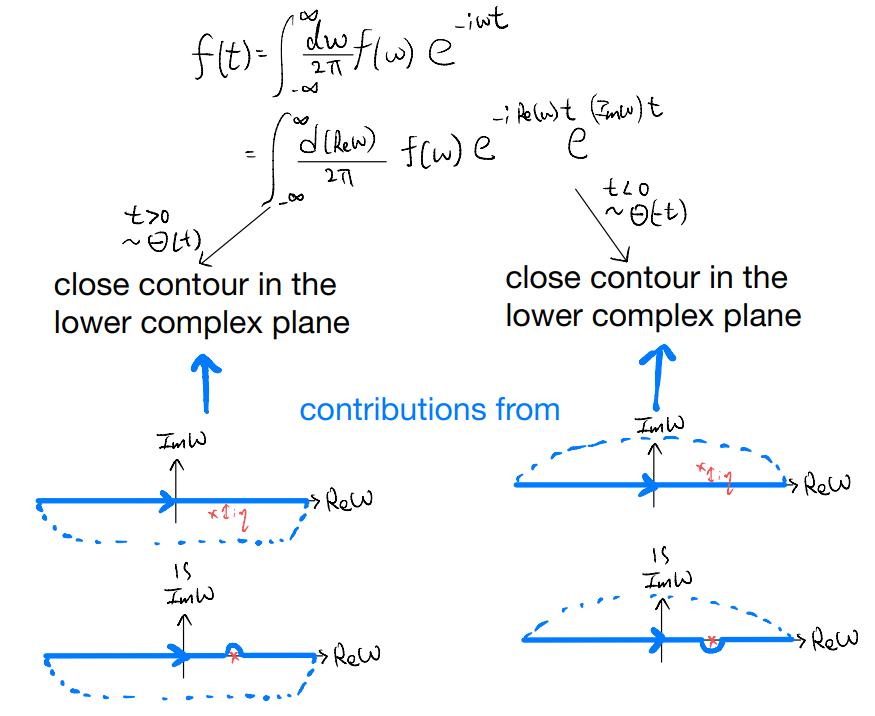
\includegraphics[width=\textwidth]{jupyterbook/data/fig/lec12-fig10.png}
\end{figure}


\chapter{Lec13 20220318}

Topics

\begin{enumerate}
    \item Linear response
    \item Susceptibility and retarded Greens' function
\end{enumerate}

Goals

\begin{enumerate}
    \item Establishing a more precise connection between Green's function and experimental observables
\end{enumerate}

\section{Recap: reasons for thinking about Green's functions}

Let us briefly recap what we have learnt about (zero-temperature) Green's functions.

\begin{enumerate}
    \item We argued that, in real time, they could be understood simply as the matrix-element of the time-evolution operator evaluated in the ground state (``Level I'')
    \item We also showed that, in the frequency space, the Green's function contains important physical information about the ground state and its excitations (``Level II'')
    \item We then see that specific ``time-ordered'' combination of the real-time Green's function form the basic ingredients when we try to solve equation of motion with time-dependent operator ``coefficients'', which leads to the time-ordered exponential (``Level III'')
    \item We just saw that, in fact, all these Green's functions are really the same in the frequency space, but just with different contour prescription in going to the real time (at least for free phonons)!
\end{enumerate}

In particular, we saw that when we close the contour on the lower complex plane, we get the ``retarded Green's function'' taking the form
\[ G^{\mathrm{ret}}\left( q,t \right) =\left( -i \right) \Theta \left( t \right) \left< \left[ \hat{A}\left( t \right) ,\hat{B}\left( 0 \right) \right] \right> \]
It has a sense of causality, in that it is non-vanishing only for $t>0$. Furthermore, when $\hat{A}$ and $\hat{B}$ are Hermitian,
\begin{align*}
    \left( -i\left[ \hat{A}\left( t \right) ,\hat{B}\left( 0 \right) \right] \right) ^{\dagger}&=\left( -i\hat{A}\left( t \right) \hat{B}\left( 0 \right) +i\hat{B}\left( 0 \right) \hat{A}\left( t \right) \right) ^{\dagger}\\
    &=i\hat{B}\left( 0 \right) \hat{A}\left( t \right) -i\hat{A}\left( t \right) \hat{B}\left( 0 \right) \\
    &=-i\left[ \hat{A}\left( t \right) ,\hat{B}\left( 0 \right) \right]
\end{align*}
this implies our retarded Green's function could be measurable! Note how things start to fall into place: the mysterious ``conventional factor'' $(-i)$ now makes sense too!

\section{Linear response}

Let us now consider a general problem and see how, indeed, the retarded Green's functions appear as the response of a system to perturbations.

Consider a static Hamiltonian $\hat{H}_0$ which wee disturb at some time by a perturbation $\hat{V}(t)$. The full Hamiltonian is given by
\[ \hat{H}\left( t \right) =\hat{H}_0+\hat{V}\left( t \right) \]
in the Schrodinger picture, i.e., the Schrodinger states evolve as
\[ i\partial _t|\Psi_S \left( t \right) \rangle=\hat{H}\left( t \right) |\Psi_S \left( t \right) \rangle\]
Taking the perspective that ``the system'' is simply described by $\hat{H}_0$ and $\hat{V}(t)$ is only ``a probe'', it will be natural to try going into a Heisenberg picture defined using $\hat{H}_0$ (instead of $\hat{H}(t)$). Consider an operator $\hat{O}$ which is time-independent in the Schrodinger picture:
\[ \langle \Psi_S \left( t \right) |\hat{O}_S|\Psi_S \left( t \right) \rangle =\langle \Psi_S \left( t \right) |e^{-i\hat{H}_0t}\left( e^{i\hat{H}_0t}\hat{O}_Se^{-i\hat{H}_0t} \right) e^{i\hat{H}_0t}|\Psi_S \left( t \right) \rangle\]
\[ \hat{O}_I\left( t \right) =e^{i\hat{H}_0t}\hat{O}_Se^{-i\hat{H}_0t}\]
where $\hat{O}_I(t)$ is equivalently Heisenberg picture for $\hat{O}$ defined using $\hat{H}_0$. Of course, this is something like a hybrid picture, because ultimately our full Hamiltonian (and so the ``true'' Heisenberg picture) also contains the perturbation.

We call this the ``interaction picture''. The equations of motions are now
\[ i\partial _t\hat{O}_I\left( t \right) =\left[ \hat{O}_I\left( t \right) ,\hat{H}_0 \right] \]
same as the Heisenberg picture for the unperturbed system.
\begin{align*}
    i\partial _t|\Psi_I \left( t \right) \rangle&=i\partial _t\left( e^{i\hat{H}_0t}|\Psi_S \left( t \right) \rangle \right) \\
    &=-\hat{H}_0\left( e^{i\hat{H}_0t}|\Psi_S \left( t \right) \rangle  \right) +e^{i\hat{H}_0t}\left( i\partial _t|\Psi_S \left( t \right) \rangle \right) \\
    &=-\hat{H}_0|\Psi_I \left( t \right) \rangle+e^{i\hat{H}_0t}\left( \hat{H}_0+\hat{V}\left( t \right) \right) e^{-i\hat{H}_0t}|\Psi_I \left( t \right) \rangle\\
    &=\hat{V}_I\left( t \right) |\Psi_I \left( t \right) \rangle
\end{align*}
\[ \hat{V}_I\left( t \right) =e^{i\hat{H}_0t}\hat{V}\left( t \right) e^{-i\hat{H}_0t}\]
i.e., the ``effective Hamiltonian'' for $|\Psi_I(t)\rangle$ is simply the perturbation, but with the operators acquiring additional time-dependence according to the Heisenberg picture of the unperturbed system. (Note: this holds even if $\hat{V}$ itself is time-independent to start with.)

We have seen already how such equation of motion could be solved: the (formal) solution is simply the time-ordered exponential:
\[ |\Psi _I\left( t \right) \rangle =\mathcal{T} \left[ e^{-i\int_{t_0}^t{dt'\hat{V}_I\left( t' \right)}} \right] |\Psi _I\left( t_0 \right) \rangle \]
In particular, at $t_0\to -\infty$ we simply have the original ground state $|\Omega\rangle$ of the unperturbed system $\hat{H}_0$, so
\[ |\Psi _I\left( t \right) \rangle =\mathcal{T} \left[ e^{-i\int_{-\infty}^t{dt'\hat{V}_I\left( t' \right)}} \right] |\Omega \rangle \]
We are now all set-up to consider how the system responds to the perturbations! As discussed, the expectation value of a physical observable is
\[ O\left( t \right) =\langle \Psi _I\left( t \right) |\hat{O}_I\left( t \right) |\Psi _I\left( t \right) \rangle \]
We could evaluate it as a perturbation series in powers of $\hat{V}$. Recall, $\hat{O}_I(t)$ is simply equivalently to the unperturbed Heisenberg operator, and so the lowest order term comes from
\begin{align*}
    |\Psi _I\left( t \right) \rangle &=\mathcal{T} \left[ e^{-i\int_{-\infty}^t{dt'\hat{V}_I\left( t' \right)}} \right] |\Omega \rangle \\
    &=\left( I-i\int_{-\infty}^t{dt'\hat{V}_I\left( t' \right)}+\cdots \right) |\Omega \rangle
\end{align*}
\begin{align*}
    O\left( t \right) &=\langle \Omega |\left( I+i\int_{-\infty}^t{dt'\hat{V}_I\left( t' \right)}+\cdots \right) \hat{O}_I\left( t \right) \left( I-i\int_{-\infty}^t{dt'\hat{V}_I\left( t' \right)}+\cdots \right) |\Omega \rangle \\
    &\approx \langle \Omega |\hat{O}_I\left( t \right) |\Omega \rangle -i\langle \Omega |\left[ \hat{O}_I\left( t \right) ,\int_{-\infty}^t{dt'\hat{V}_I\left( t' \right)} \right] |\Omega \rangle
\end{align*}
\begin{align*}
    \delta O\left( t \right) &=O\left( t \right) -\langle \Omega |\hat{O}_S|\Omega \rangle \\
    &=O\left( t \right) -\langle \Omega |\hat{O}_I\left( t \right) |\Omega \rangle \\
    &=-i\langle \Omega |\left[ \hat{O}_I\left( t \right) ,\int_{-\infty}^t{dt'\hat{V}_I\left( t' \right)} \right] |\Omega \rangle
\end{align*}
This relates the change in the observable to the lowest (linear) order in the perturbation $\hat{V}$. Let us further assume the perturbation takes the form
\[ \hat{V}_S\left( t \right) =\hat{O}_{S}^{'}f\left( t \right) \]
\[ \Rightarrow \hat{V}_I\left( t \right) =\hat{O}_{I}^{'}f\left( t \right) \]
i.e., its only time-dependence in the Schrodinger picture comes solely from a time-dependent ``driving force'' $f(t)$.

Our discussions simplify further in the frequency space. Consider the Fourier transform of the force
\[ f\left( t \right) =\int_{-\infty}^{\infty}{\frac{d\omega}{2\pi}f\left( \omega \right) e^{-i\omega t}}\]
\begin{align*}
    \Rightarrow \delta O\left( t \right) &=\left( -i \right) \int_{-\infty}^t{dt'\langle \Omega |\left[ \hat{O}_I\left( t \right) ,\hat{O}_{I}^{'}\left( t' \right) \right] |\Omega \rangle \int_{-\infty}^{\infty}{\frac{d\omega}{2\pi}f\left( \omega \right) e^{-i\omega t'}}}\\
    &=\int_{-\infty}^{\infty}{\frac{d\omega}{2\pi}f\left( \omega \right) \left( -i \right) \int_{-\infty}^t{dt'\langle \Omega |\left[ \hat{O}_I\left( t \right) ,\hat{O}_{I}^{'}\left( t' \right) \right] |\Omega \rangle e^{-i\omega t'}}}
\end{align*}
\[ \langle \Omega |\left[ \hat{O}_I\left( t \right) ,\hat{O}_{I}^{'}\left( t' \right) \right] |\Omega \rangle =\langle \Omega |\left[ \hat{O}_I\left( t-t' \right) ,\hat{O}_{I}^{'}\left( 0 \right) \right] |\Omega \rangle \]
where the time-translation invariance follows from a static non-perturbed $\hat{H}_0$, and that our interaction picture operators are simply the Heisenberg picture operators with respect to $\hat{H}_0$. Let $\delta_t=t-t'>0$, then
\begin{align*}
    &\int_{-\infty}^t{dt'\left( -i \right) \langle \Omega |\left[ \hat{O}_I\left( t-t' \right) ,\hat{O}_{I}^{'}\left( 0 \right) \right] |\Omega \rangle e^{-i\omega t'}}\\
    &=\left( \int_0^{\infty}{d\delta _t\left( -i \right) \langle \Omega |\left[ \hat{O}_I\left( \delta _t \right) ,\hat{O}_{I}^{'}\left( 0 \right) \right] |\Omega \rangle e^{i\omega \delta _t}} \right) e^{-i\omega t}
\end{align*}
Let us define the susceptibility
\[ \chi \left( \omega \right) =\int_{-\infty}^{\infty}{d\delta _t\left( -i \right) \Theta \left( \delta _t \right) \langle \Omega |\left[ \hat{O}_I\left( \delta _t \right) ,\hat{O}_{I}^{'}\left( 0 \right) \right] |\Omega \rangle e^{i\omega \delta _t}}\]
where we have again traded the integration bound with the Heaviside step function.

Importantly, notice that $\chi(\omega)$ is simply the frequency-space version of some retarded Green's function!

When the dust settles, we arrive at
\[ \delta O\left( t \right) =\int_{-\infty}^{\infty}{\frac{d\omega}{2\pi}\chi \left( \omega \right) f\left( \omega \right) e^{-i\omega t}}\]
and so, when we Fourier transform the observable, we get
\[ \delta O\left( \omega \right) =\chi \left( \omega \right) f\left( \omega \right) \]
\[ \Rightarrow \quad \chi \left( \omega \right) =\frac{\delta O\left( \omega \right)}{f\left( \omega \right)}\]
i.e., the susceptibility is measurable simply as the ratio of the Fourier component of the (change in the) observable and the driving force we used to perturb the system, and it is given by
\[ \chi \left( \omega \right) =\int_{-\infty}^{\infty}{dt\chi _R\left( t \right) e^{i\omega t}}\]
\[ \chi _R\left( t \right) =\left( -i \right) \Theta \left( t \right) \langle \Omega |\left[ \hat{O}_I\left( t \right) ,\hat{O}_{I}^{'}\left( 0 \right) \right] |\Omega \rangle ,\quad \mathrm{retarded}\]
Such relationships (linear-response susceptibilities to retarded Green's functions) are called ``Kubo formulas''. It is customary to split it into real and imaginary parts:
\[ \chi \left( \omega \right) =\Re \left[ \chi \left( \omega \right) \right] +i\Im \left[ \chi \left( \omega \right) \right] \]
\[ \Re \left[ \chi \left( \omega \right) \right] =\int_{-\infty}^{\infty}{\chi _R\left( t \right) \cos \left( \omega t \right)}\]
\[ \Im \left[ \chi \left( \omega \right) \right] =\int_{-\infty}^{\infty}{\chi _R\left( t \right) \sin \left( \omega t \right)}\]
From which we see that the real part is an even function of $\omega$, whereas the imaginary part is odd. Therefore, we may also simply write
\[ \Re \left[ \chi \left( \omega \right) \right] =\frac{\chi \left( \omega \right) +\chi \left( -\omega \right)}{2}\]
\[ \Im \left[ \chi \left( \omega \right) \right] =\frac{\chi \left( \omega \right) -\chi \left( -\omega \right)}{2i}\]
You might recall that, the imaginary susceptibility corresponds to energy dissipation / absorption. To see why, let us consider a ``monochromatic'' drive
\[ f\left( t \right) =f_0\cos \left( \Omega t \right) \]
\[ f\left( \omega \right) =\pi f_0\delta \left( \omega +\Omega \right) +\pi f_0\delta \left( \omega -\Omega \right) \]
Correspondingly, the change in the physical observable is
\begin{align*}
    \delta O\left( t \right) &=\int_{-\infty}^{\infty}{\frac{d\omega}{2\pi}\chi \left( \omega \right) f\left( \omega \right) e^{-i\omega t}}\\
    &=\int_{-\infty}^{\infty}{\frac{d\omega}{2}f_0\chi \left( \omega \right) \left( \delta \left( \omega +\Omega \right) +\delta \left( \omega -\Omega \right) \right) e^{-i\omega t}}\\
    &=\frac{f_0}{2}\chi \left( \Omega \right) e^{-i\Omega t}+\frac{f_0}{2}\chi \left( -\Omega \right) e^{i\Omega t}\\
    &=f_0\cos \left( \Omega t \right) \Re \left[ \chi \left( \Omega \right) \right] +f_0\sin \left( \Omega t \right) \Im \left[ \chi \left( \Omega \right) \right]
\end{align*}
In other words, the real part $\Re[\chi(\omega)]$ corresponds to the in-phase (also known as reactive) response, whereas the imaginary part $\Im[\chi(\omega)]$ corresponds to the out-of-phase response. As you might recall, the out-of-phase response corresponds to energy dissipation / absorption. To see that, let us consider a generalized power
\begin{align*}
    P\left( t \right) &=f\left( t \right) \frac{d}{dt}\delta O\left( t \right) ,\quad \left( \mathrm{c}.\mathrm{f}. P=Fv=F\frac{dx}{dt} \right) \\
    &=f_{0}^{2}\cos \left( \Omega t \right) \frac{d}{dt}\left( \Re \left[ \chi \left( \Omega \right) \right] \cos \left( \Omega t \right) +\Im \left[ \chi \left( \Omega \right) \right] \sin \left( \Omega t \right) \right) \\
    &=f_{0}^{2}\Omega \left( -\Re \left[ \chi \left( \Omega \right) \right] \cos \left( \Omega t \right) \sin \left( \Omega t \right) +\Im \left[ \chi \left( \Omega \right) \right] \cos ^2\left( \Omega t \right) \right) \\
    &=\frac{f_{0}^{2}\Omega}{2}\left( -\Re \left[ \chi \left( \Omega \right) \right] \sin \left( 2\Omega t \right) +\Im \left[ \chi \left( \Omega \right) \right] \cos \left( 2\Omega t \right) +\Im \left[ \chi \left( \Omega \right) \right] \right)
\end{align*}
When we average the power over one period of the drive, the only survive piece is
\[ \left< P\left( t \right) \right> =\pi f_{0}^{2}\Im \left[ \chi \left( \Omega \right) \right] \]
this shows explicitly the imaginary (the odd-in-frequency) part of the susceptibility captures the dissipation / absorption of the system.

These are very general conclusions, and, in fact, apply similarly even to systems at finite temperature. In particular, it provides a general platform for understanding the response, fluctuation, and dissipation in a system.

Let us now unpack these formal calculations by considering a ``canonical'' example.

\section{Driven QHO}

As our first example, let us consider again our old friend now perturbed by a driving term
\[ \hat{H}_0=\frac{\hat{p}^2}{2m}+\frac{1}{2}m\omega _{0}^{2}\hat{x}^2-\frac{1}{2}\omega _0=\omega _0\hat{a}^{\dagger}\hat{a}\]
\[ \hat{a}=\frac{1}{\sqrt{2}}\left( \sqrt{m\omega _0}\hat{x}+i\frac{\hat{p}}{\sqrt{m\omega _0}} \right) \]
\[ \hat{V}_s=f\left( t \right) \hat{x}\]
Let us consider how the position of the particle responds to the drive, i.e., we look at the susceptibility
\begin{align*}
    \chi \left( t \right) &=\left( -i \right) \Theta \left( t \right) \langle 0|\left[ \hat{x}\left( t \right) ,\hat{x}\left( 0 \right) \right] |0\rangle \\
    &=\frac{\left( -i \right) \Theta \left( t \right)}{2m\omega _0}\langle 0|\left[ \hat{a}\left( t \right) +\hat{a}^{\dagger}\left( t \right) ,\hat{a}\left( 0 \right) +\hat{a}^{\dagger}\left( 0 \right) \right] |0\rangle \\
    &=\frac{\left( -i \right) \Theta \left( t \right)}{2m\omega _0}\left( e^{-i\omega _0t}-e^{i\omega _0t} \right) \\
    &=-\frac{\Theta \left( t \right)}{m\omega _0}\sin \left( \omega _0t \right)
\end{align*}
Hopefully this looks familiar. We already saw that it corresponds to the frequency-space pole structure

\begin{figure}[ht]
    \centering
    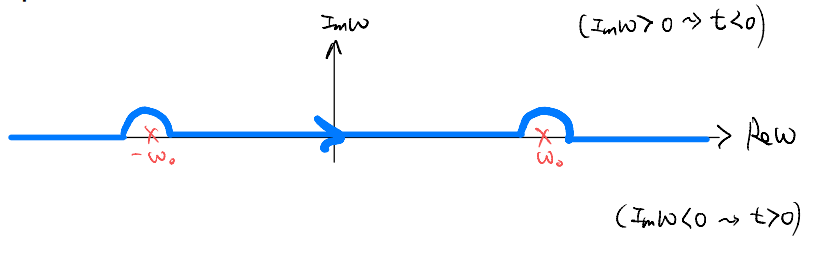
\includegraphics[width=\textwidth]{jupyterbook/data/fig/lec13-fig00.png}
\end{figure}

In the $i\eta$ prescription, we have
\begin{align*}
    \chi \left( \omega \right) &=\frac{1}{2m\omega _0}\lim_{\eta \rightarrow 0^+} \left( \frac{1}{\omega -\omega _0+i\eta}-\frac{1}{\omega +\omega _0+i\eta} \right) \\
    &=\frac{1}{2m\omega _0}\lim_{\eta \rightarrow 0^+} \frac{2\omega _0}{\left( \omega +i\eta \right) ^2-\omega _{0}^{2}}\\
    &=\frac{1}{m}\lim_{\eta \rightarrow 0^+} \frac{1}{\omega ^2-\omega _{0}^{2}+2i\omega \eta}
\end{align*}
This may look familiar to you: the response has a strong peak at the natural frequency, with the peak width controlled by $i\eta$.

Furthermore, we can extract the imaginary part. Recall the Sokhotski-Plemelj theorem
\[ \lim_{\eta \rightarrow 0^+} \frac{1}{x\pm i\eta}=P\frac{1}{x}\mp i\pi \delta \left( x \right) \]
\begin{align*}
    \Rightarrow \quad \Im \left[ \chi \left( \omega \right) \right] &=\frac{1}{2m\omega _0}\Im \left[ \lim_{\eta \rightarrow 0^+} \left( \frac{1}{\omega -\omega _0+i\eta}-\frac{1}{\omega +\omega _0+i\eta} \right) \right] \\
    &=\frac{\pi}{2m\omega _0}\left( -\delta \left( \omega -\omega _0 \right) +\delta \left( \omega +\omega _0 \right) \right)
\end{align*}
Earlier, we introduced this as the ``spectral'' function, obtained by the spectral decomposition for a general many-body Hamiltonian, which could be understood as the matrix-element-weighed density of states. Here, we see that, indeed, it corresponds to experimental observables.


\end{document}
